% !TeX root = ../main.tex
% Add the above to each chapter to make compiling the PDF easier in some editors.

\chapter{\glsentrytext{holoassist}}\label{chapter:holoassist}

As explained in \autoref{section:problemstatement} the main aim of this thesis is to build a solution that allows to easily display arbitrary augmentations in a fixed-platform flight simulator. The best way to achieve this result was to build \enquote{\gls{holoassist}}, a Hololens application developed using the Unity game engine that contains all the logic that is necessary to display a desired 3D mesh:

\begin{enumerate}
    \item at a specific real-world location identified by some geographic coordinates, so that by wearing the Hololens inside the flight simulator and looking \enquote{outside} the cockpit window one would see that 3D mesh anchored to that specific geographical location. This type of augmentation is called \enquote{\gls{geofixedaug}};
    \item at a specific location inside the flight simulator cockpit, so that by wearing the Hololens and looking at that specific point one would see the 3D mesh anchored to it. This type of augmentation is called \enquote{\gls{planefixedaug}}.
\end{enumerate}

Since developing directly for the Hololens is not trivial for someone with limited computer science experience, decoupling the creation of the augmentations from \gls{holoassist} seemed to be the best approach. Therefore, \gls{holoassist} exposes a generic \gls{API} that can be used to draw arbitrary augmentations: the specific instances of the augmentations are created, drawn and handled by external scripts, called \glspl{holoassistapp}.  These scripts use the \gls{holoassist} \gls{API} via the local network and are relatively easy to develop also for someone with limited programming experience: an minimal \glspl{holoassistapp} that can highlight a specific runway at an airport can be written in just fifteen lines of Python. A diagram outlining the overall data flow is available in \autoref{fig:dataflow_diagram}.

\begin{figure}
  \centering
  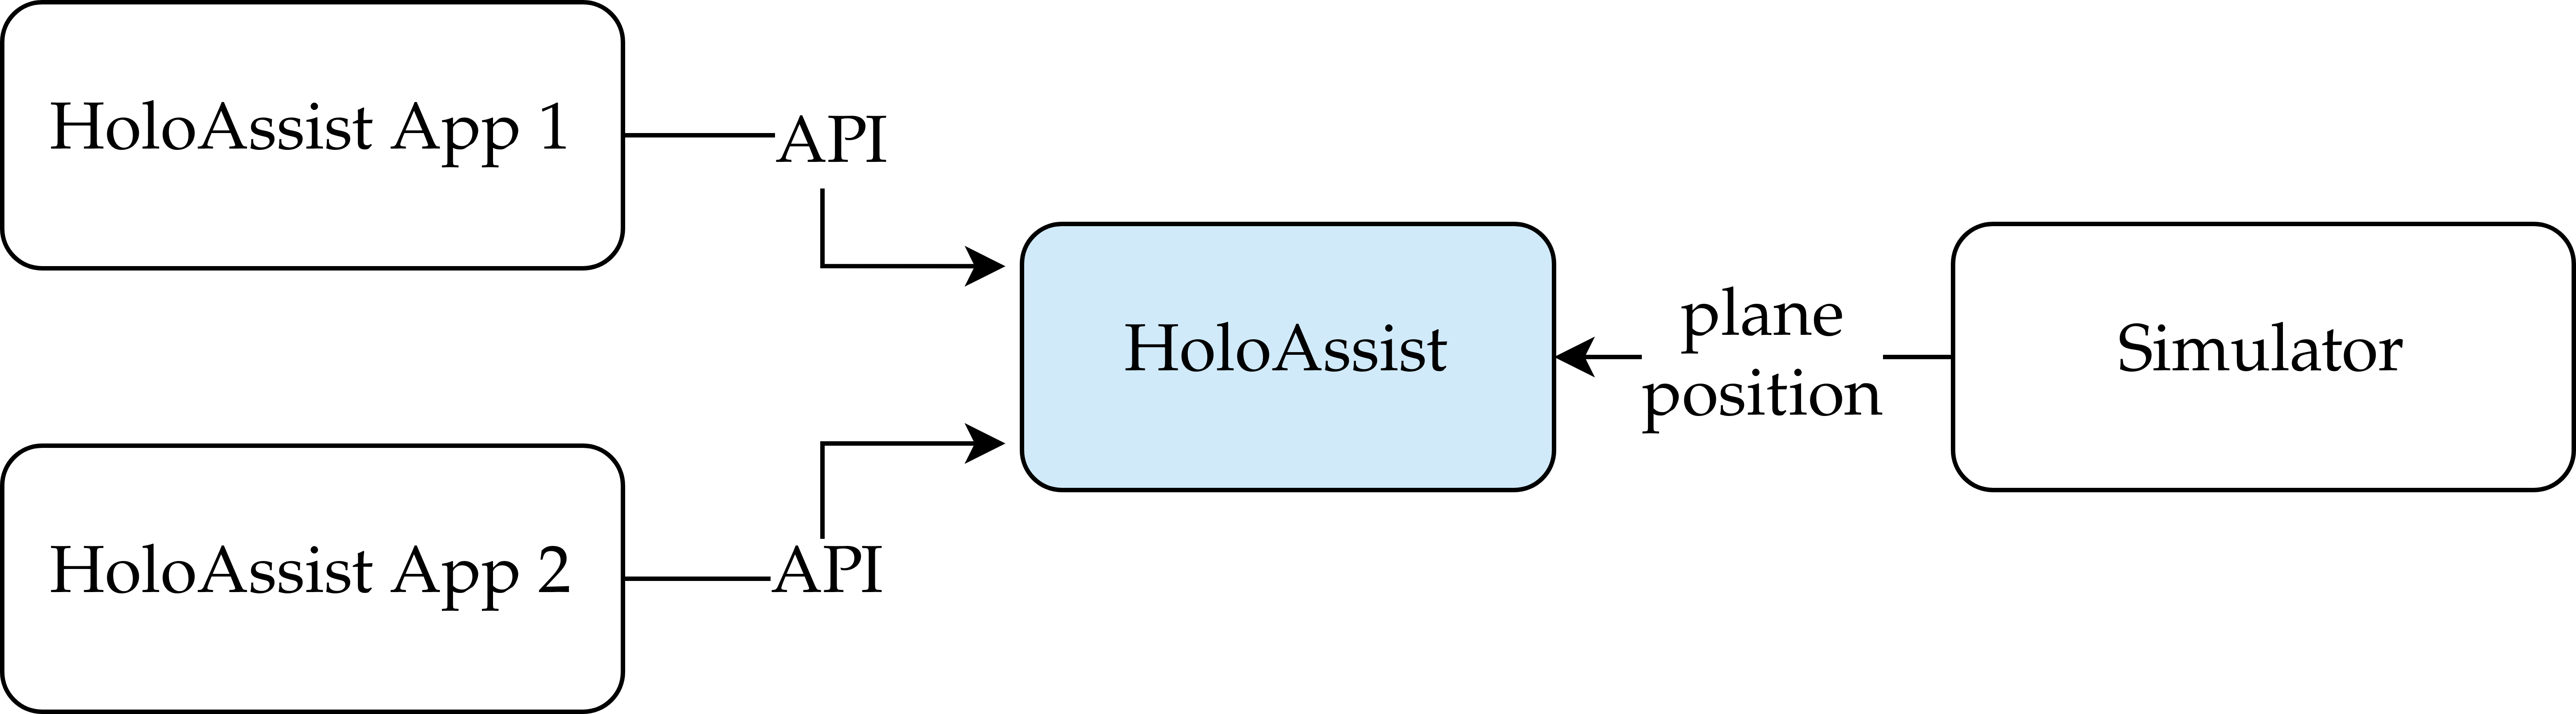
\includegraphics[width=0.8\textwidth]{dataflow_diagram.png}
  \caption{A graphical representation of the interaction between \gls{holoassist}, \glspl{holoassistapp} and the flight simulator being used. All interactions happen through the local network. \gls{holoassist} runs on the Hololens, whereas the various \gls{holoassistapp} run on a normal computer.}\label{fig:dataflow_diagram}
\end{figure}

\section{Aligning the virtual 3D world with the real one}\label{section:aligning_virtual_with_real_world}

The first problem to tackle was to align \gls{holoassist}'s 3D world with the real one. When a Unity application is started on the Hololens, the device establishes a world-fixed coordinate system centered at its current real-world position. This world-fixed coordinate system is then used by the game engine to position its own root coordinate system. Therefore, a 3D cube that is placed in Unity's root coordinate system at the point $(0, 0, 0)^T$ will appear in different real-world positions, depending on where the Hololens is in the real world when the user starts the Unity application. This is sufficient in many situations, but makes \gls{holoassist}'s use case more difficult, because correctly placing the augmentations requires aligning them with the real-world flight simulator.

The first solution attempt relied on a manual alignment performed by the user on application startup: the user would start \gls{holoassist} and then use their hand to grab a virtual pointer that would appear in front of them. The user would then move this virtual pointer with their hand until it was aligned with the real world corner of the simulator it represented: its new pose in the virtual world would then be used to position all the other scene objects. Unfortunately, this approach did not work at all. Aligning virtual and real world items in \gls{AR} is a difficult problem\cite{martin-gomez_augmented_2020} and it led to very poor results, especially since this would have to be done every time \gls{holoassist} was started. This solution was therefore quickly discarded.

Since the Hololens has dedicated hardware to recognize QR codes and to estimate their real world pose, it can perform this task very efficiently\footnote{Opposed to approaches like the one used by the Vuforia library\cite{ptc_inc_vuforia_nodate}, which uses the Hololens camera directly and performs the QR code recognition and pose estimation in software.} (see \autoref{fig:first_experiments_with_hololens}). It was therefore decided to attach a single QR code to the flight simulator and use this custom hardware to recognize it and locate it in the virtual world. This estimated pose was then used to update the virtual-world position of a Unity object so that it would match the real-world QR code. This object would then be used to position all the other required elements in the real world. 

\begin{figure}
  \centering
  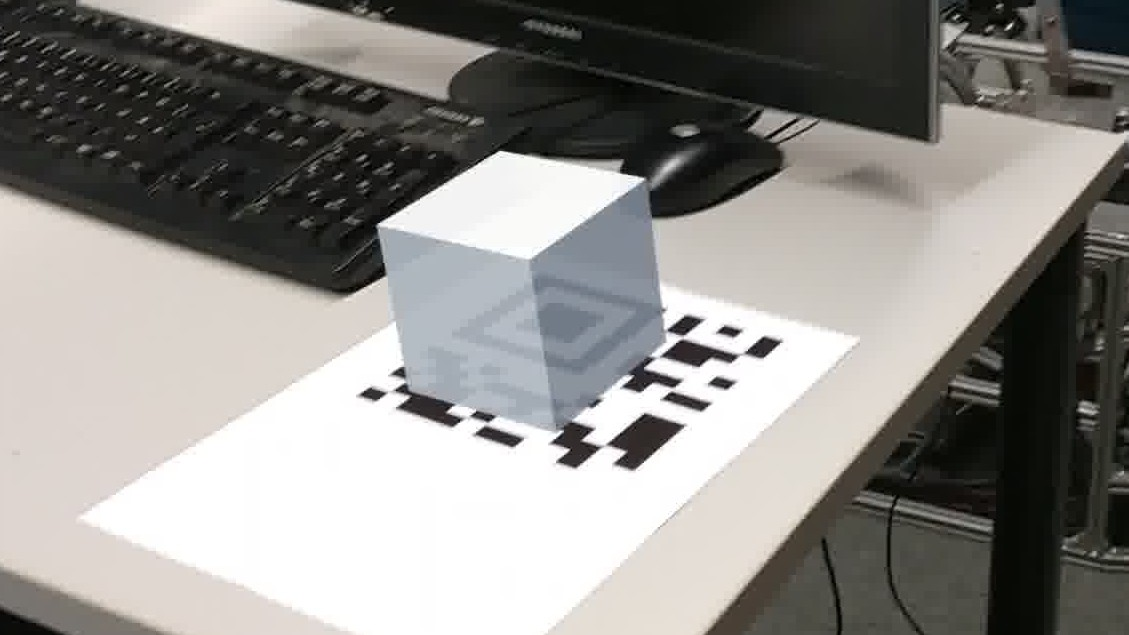
\includegraphics[width=0.6\textwidth]{first-experiment-with-qr-code.jpg}
  \caption{A picture taken from the Hololens point of view of the first tests with its QR code detection hardware. This is also an example of how important the occlusion clue is for the authenticity of augmentations: although the cube is correctly placed with its center around the top-left corner of the QR code, it \enquote{looks wrong} due to the fact that the part of it below the piece of paper is not occluded by it.}\label{fig:first_experiments_with_hololens}
\end{figure}

The result was extremely more pleasant to use, less cumbersome, faster and more precise than the manual approach, but it was still sub-optimal: the pose estimation of the QR code is not perfect, especially as far as rotation is concerned. Due to how \gls{geofixedaug} are processed (see \autoref{section:geofixedaugmentations}), they are very sensitive to errors in the rotational component of the alignment between the real and virtual world, and the precision offered by a single QR code was not sufficient. Therefore, it was decided to try to use multiple QR codes instead of a single one. This led to the discovery of the \gls{WLT}\cite{microsoft_corporation_world_nodate}, developed by Microsoft to solve a slightly different problem but that could work also for \gls{holoassist}'s use case. \gls{WLT} solves the problem of providing a \enquote{frozen} Unity coordinate system, which remains fixed with respect to real world features also across application reboots and large-scale movements of the Hololens in the real world.

The Hololens \gls{API} natively offers a way to pin a virtual 3D object to a real world location via the mechanism of \enquote{spatial anchors}. While the application is running, it can request to the device a spatial anchor to a real-world point. After such request, the Hololens starts tracking that real-world point, continuously updating the virtual-world pose of virtual objects bound to the returned spatial anchor to correct for sensor errors. However, this only works if the spatial anchor remains close to the Hololens (less than around three meters). Moreover, corrections will be applied to each spatial anchor individually. Therefore, even though two real-world point are in a fixed position with respect to each other, two spatial anchors bound to those point will not necessarily remain fixed relative to each other. Given these limitations, using multiple spatial anchors across large-scale \gls{AR} experiences is difficult, because clusters of virtual objects bound to different spatial anchors will drift away relative to each other as the real world points referenced by the spatial anchors leave the field of view of the Hololens.

The \acrlong{WLT} solves this problem by introducing the concepts of \enquote{frozen}, \enquote{locked} and \enquote{spongy} spaces. The default Unity coordinate system, where each individual anchor is free to move independently from all the others, is called spongy space, because reference points are continuously updated by the sensor refinements. For every frame, the Frozen World Engine offered by the library computes a rigid transformation that converts from the spongy space to the so-called locked space, a different Cartesian coordinate space which is as stable as possible, meaning that a stationary object placed in it will remain fixed with respect to real world features. However, the origin of this space is arbitrary. More formally\footnote{The following derivation is a plausible simplification of what is actually done by the \gls{WLT} and is obtained from the library's documentation. Describing the exact implementation is impractical as it is closed-source and owned by Microsoft.}, let $\mathbf{a}_i^t$ be the position in spongy space of the $i$-th spatial anchor at frame $t$ and $T_{SL}^t$ be the transformation matrix from spongy space to locked space for frame $t$. Then for frame $t+1$ \gls{WLT} is trying to compute $T_{SL}^{t+1}$ such that:

\begin{equation}
T_{SL}^{t+1} = \argmin_{T_{SL}^{t+1}} \sum_i \left(\frac{d_i^t + d_i^{t+1}}{2}\right)^{-1} \left\lVert T_{SL}^t \mathbf{a}_i^t - T_{SL}^{t+1} \mathbf{a}_i^{t+1} \right\rVert
\end{equation}

Where $T_{SL}^t \mathbf{a}_i^t$ is the position in locked space of anchor $\mathbf{a}_i$ at frame $t$ and $T_{SL}^{t+1} \mathbf{a}_i^{t+1}$ is the position in locked space of anchor $\mathbf{a}_i$ at frame $t+1$. The value $d_i^t \in \mathbb{R}$ is the real-world distance between the anchor $\mathbf{a}_i$ and the Hololens at frame $t$, and is used as a weighting factor to give more importance to the anchors that are closer to the device, as those are the ones for which the sensors have likely been able to determine a more precise position.

However, there are infinite valid locked spaces: any rigid transform applied to a locked space will yield another locked space. To transform from a locked space to the frozen space, persistent across reboots and large-scale movements, \gls{WLT} introduces the concept of \enquote{space pins}. A space pin is a virtual-world point that corresponds to a precise location in the real-world (e.g.\ the position of the top-left corner of a QR code). The application is responsible for supplying the pose of the space pins that are detectable in the real world, and then the \gls{WLT} uses those to compute a transformation from the locked space to the frozen space in such a way that it best satisfies all the supplied space pins. More formally\footnote{Again, a plausible simplification.}, let $\mathbf{p}_i^{t}$ be the locked space position of space pin $i$ at frame $t$ and $\mathbf{q}_i$ be its desired position in the virtual (frozen) world. $\mathbf{p}_i^t$ is obtainable by applying the transformation from spongy to locked space obtained for the current frame to the currently available sensor data. The Frozen World Engine is then computing a transformation $T_{LF}^t$ from the locked space to the frozen space such that:

\begin{equation}
T_{LF}^t = \argmin_{T_{LF}^t} \sum_i \frac{1}{d_i^t}\left\lVert T_{LF}^t \mathbf{p}_i^t - \mathbf{q}_i\right\rVert
\end{equation}

Where once again $d_i^t \in \mathbb{R}$ is the distance between the $i$-th space point and the Hololens at frame $t$ and acts as a weight to give more importance to space pins closer to the device. The two computed transformations can then be combined into a single one that allows to convert spongy space poses to frozen world poses. Every frame, this combined transformation is cleverly applied to the Unity camera hierarchy in such a way that placing Unity objects normally in the game engine's root coordinate system results in them being automatically placed in the frozen space, hiding away all the complexity described above.

This behavior is exactly what is desired for \gls{holoassist}: by simply placing some QR codes in the real world and using them as space pins it is possible to obtain a very precise alignment between the virtual world and the real one. Concretely, this requires measuring the real-world offset between the QR codes with a tape measure and then use Unity's \texttt{GameObject}s to replicate their structure in the virtual world as shown in \autoref{image:qr_codes_real_world_virtual_world.png}. \gls{holoassist} then uses the Hololens \gls{API} to detect these QR codes in the real world while the application is running and supplies their pose estimate to the \gls{WLT} as space pins, matching each real world QR code with the correct \texttt{GameObject} representing the space pin in the virtual world. \gls{WLT} then takes care of the rest.

\begin{figure}[b!]
  \centering
  \subfloat[The real world QR codes]{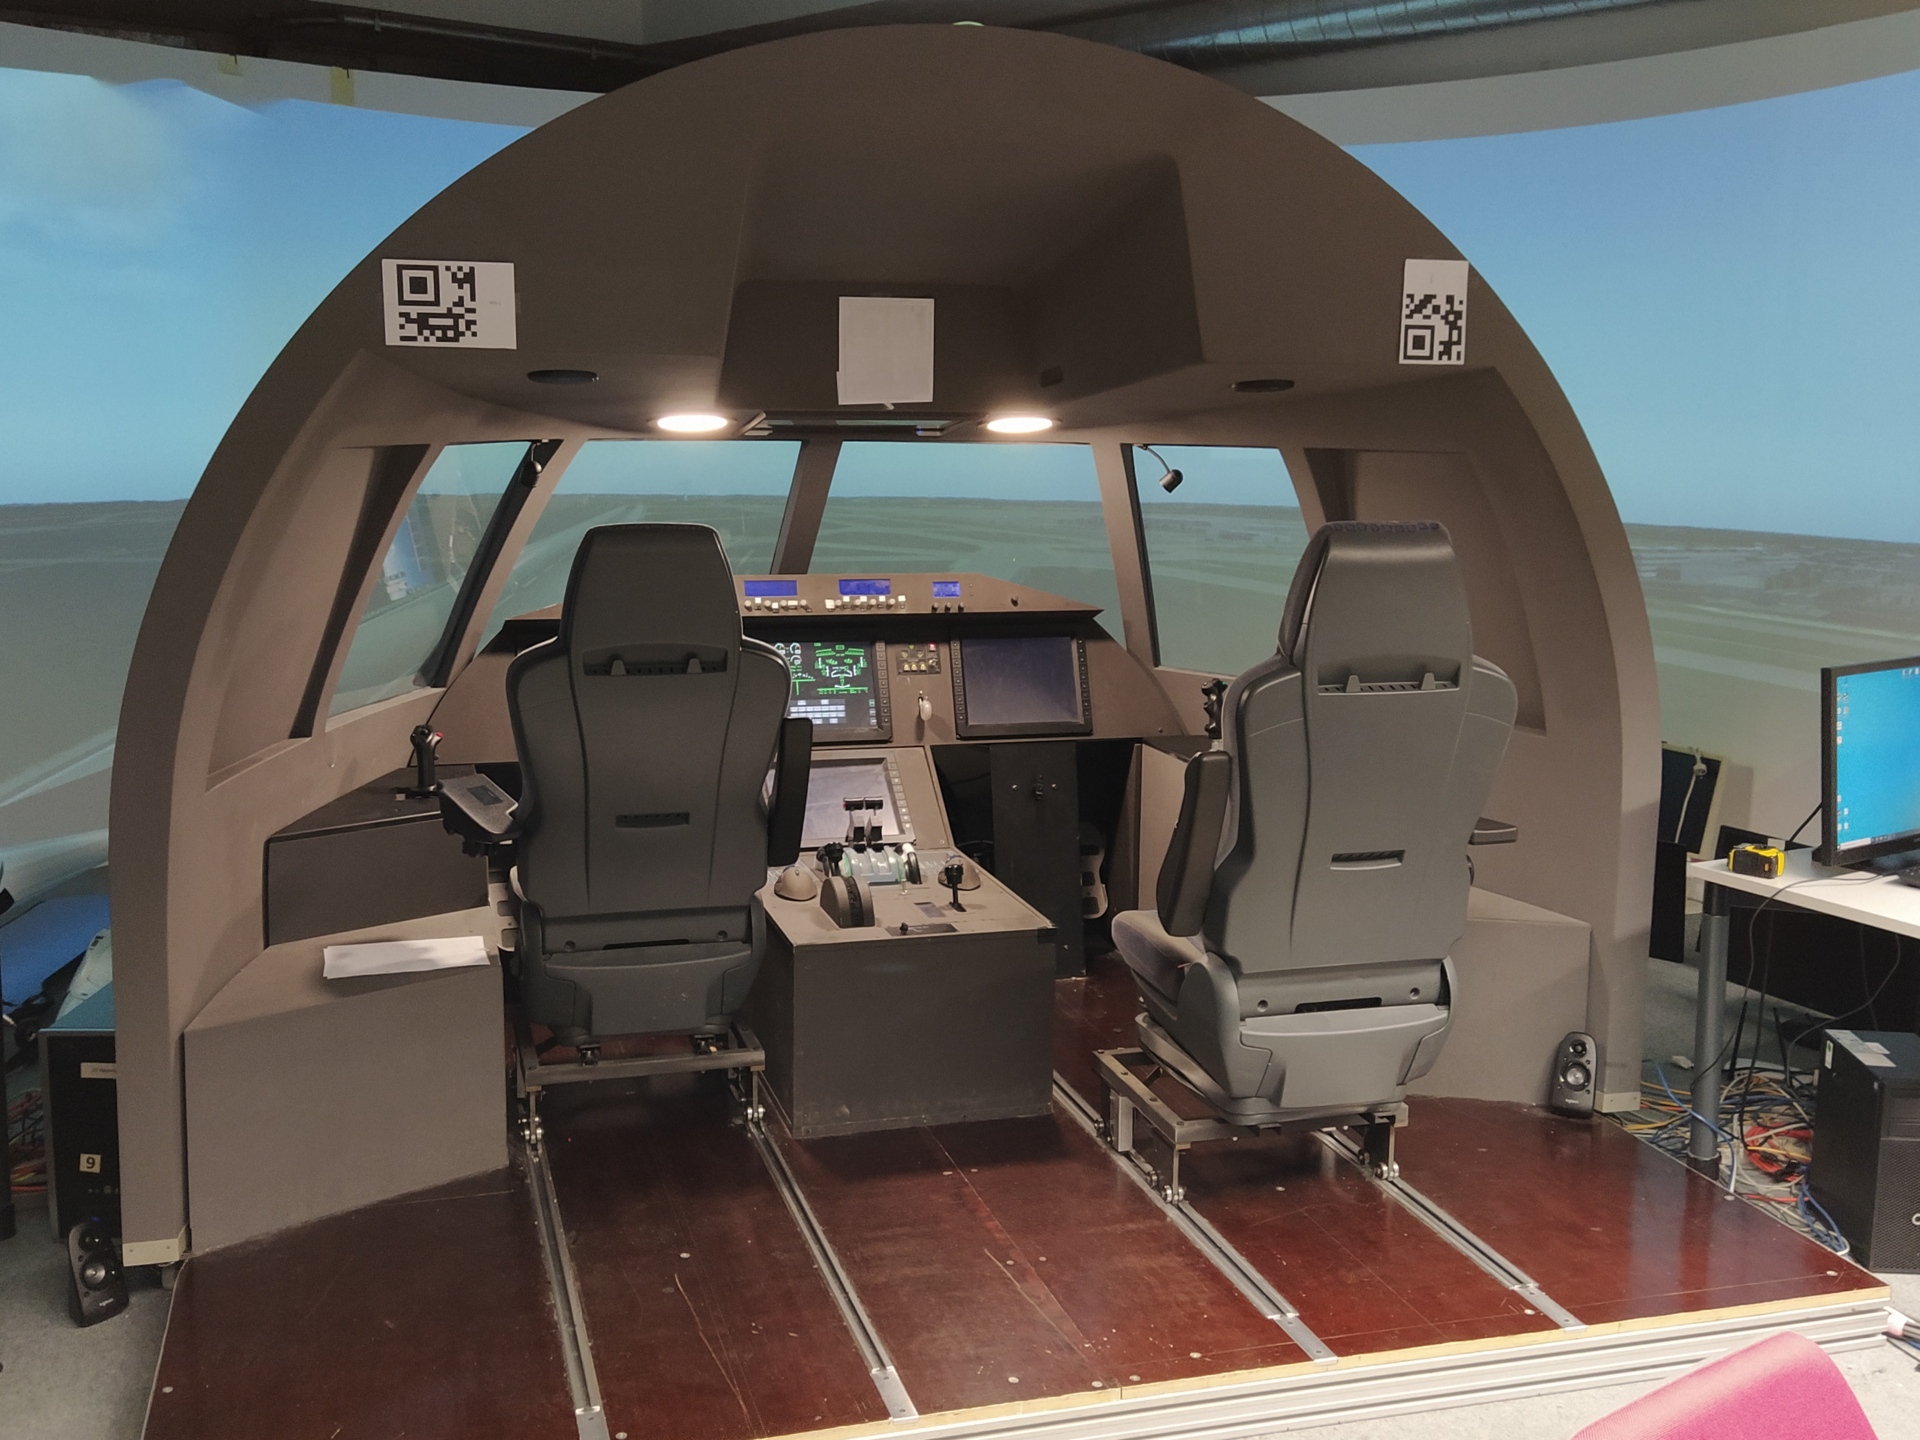
\includegraphics[height=0.35\textwidth]{the-rfs.png}}
  \hfill
  \subfloat[The virtual space pins]{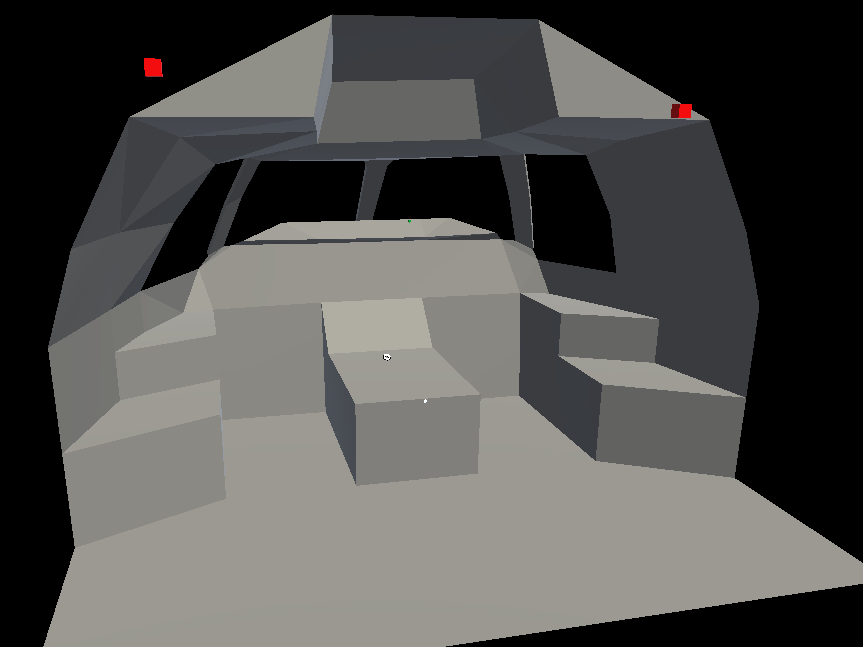
\includegraphics[height=0.35\textwidth]{qr-codes-in-unity.png}}
  \caption{The images shows how the offset between the virtual space pins in Unity (in red) should match with the offset between the real world QR codes.}\label{image:qr_codes_real_world_virtual_world.png}
\end{figure}

Testing this solution quickly revealed that the QR codes position estimated by the Hololens is not perfect: it is reasonably precise, but changes over time, apparently within a sphere centered at the correct real-world position and with a radius of about half a centimeter. This effect is particularly noticeable if the QR code is further away than one meter from the Hololens and if the room illumination is insufficient (not necessarily dark, but simply not bright enough). The concrete result of this position detection error is that the alignment computed by \gls{WLT} is sub-optimal, and easily results in visible alignment errors between real-world features and the \glspl{geofixedaug} shown on top of them. Since the reported position visually appeared to be randomly and uniformly distributed around the correct position, it was decided to filter the QR code position submitted to \gls{WLT} by averaging the last ten QR code position estimates reported from the Hololens \gls{API}. Moreover, if the distance between the Hololens and the estimated QR code position is greater than $80$cm, that measurement is discarded directly and not taken into account when computing the average. This distance threshold has been choosen empirically and is determined by the fact that the precision of the QR code pose estimation produced by the Hololens decreases with distance from the QR code itself. Applying this filtering and averaging step significantly improved the final alignment and reduced the visual difference between real-world features and augmentations. Moreover, this makes the alignment procedure completely automatic, as it only requires the user to look at the QR codes for a few seconds. If for any reason the Hololens loses tracking or the alignment is broken, simply looking again at the QR codes is sufficient to re-establish.

As \gls{holoassist} should be able to support multiple different flight simulator, the \texttt{GameObject}s that act as space pins are not hard-coded. They are generated dynamically from a JSON file in which their desired position in the virtual world is recorded. A detailed description of this JSON file is available in \autoref{sec:integrating_new_sim}. All the JSON files describing the currently supported flight simulators are packaged with the \gls{holoassist} application and the correct one is selected depending on the first QR code that is detected.

\vfill

\section{Acquiring the digital double of the simulator}\label{section:acquiring_digital_double}

\Glspl{geofixedaug} should only be displayed when the user is looking through the windows of the flight simulator's cockpit. Otherwise, they could end up covering important in-cockpit information, degrading the pilot experience instead of improving it. This can be achieved by acquiring a digital double of the simulator cockpit: this virtual 3D model could then be placed in the virtual \enquote{frozen} world described in \autoref{section:aligning_virtual_with_real_world} so that the windows of the 3D model would be aligned with the windows of the real cockpit. The remaining part of the digital double would provide the required occlusion for the rest of the cabin. 

A straightforward approach to build this digital double would be to use a tape measure and to build a \gls{CAD} model of the simulator shell with the correct dimensions. Moreover, at least for the use case of \glspl{geofixedaug} occlusion, the \gls{CAD} model does not need to be particularly detailed: as long as the general shape is correct and the window holes are in the correct position it will satisfy the requirements. However, since this approach is traditional and well-known, it was decided to use this opportunity to experiment with more innovative technologies, in order to assess their viability and potentially discover better and/or faster workflows.

A first idea was to use the \enquote{spatial awareness} functionality offered by the Hololens \gls{API}. It uses the integrated depth camera of the device to provide to the application an approximate 3D mesh of the environment surrounding the Hololens. Unfortunately, the results are not sufficient for \gls{holoassist}'s use case because:

\begin{enumerate}
    \item The simulator's cockpit windows are made of transparent glass, which sometimes is reflective enough for the Hololens to detect it as opaque geometry.
    \item The spatial awareness mesh is very imprecise, even at the highest quality setting, especially considering the small-scale details like the control inputs and buttons of the flight simulator cockpit. Although this is not strictly necessary for the \glspl{geofixedaug} occlusion, it will play a role in designing \glspl{planefixedaug} (see \autoref{section:planefixedaugmentations}).
\end{enumerate}

It is also possible to save the spatial awareness mesh to a file, with the idea of using it as a starting point to then refine manually: attempting this resulted in the mesh visible in \autoref{fig:spatial_awareness_mesh_example}. However, polishing this mesh proved to be significantly more time-intensive than expected, as it had plenty of holes and intersecting geometry. These considerations led to discard the approach based on spatial awareness.

\begin{figure}
  \centering
  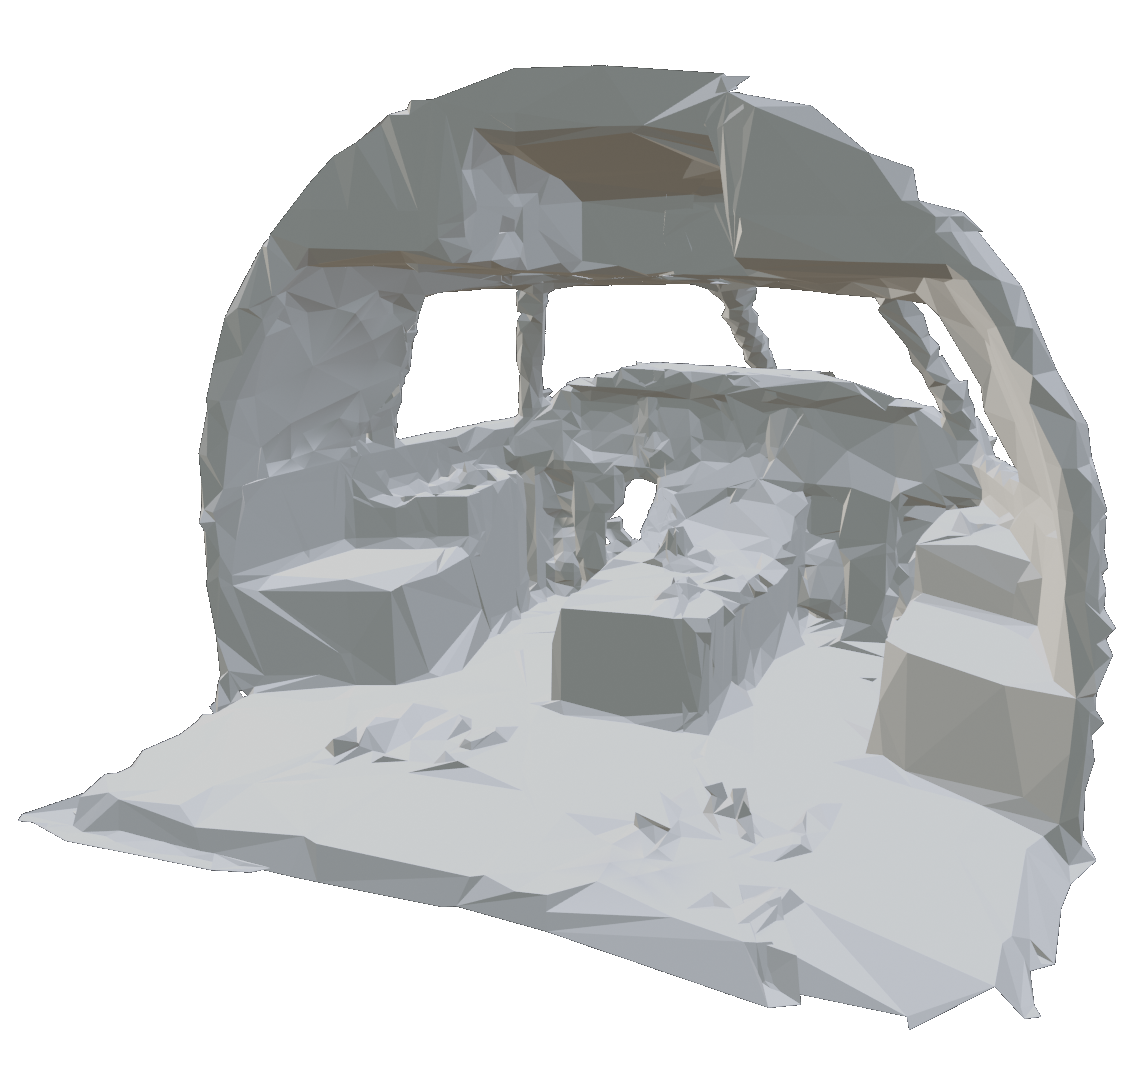
\includegraphics[width=0.5\textwidth]{spatial-awareness-mesh.png}
  \caption{The 3D scan of the simulator acquired via the spatial awareness feature of the Hololens.}\label{fig:spatial_awareness_mesh_example}
\end{figure}

Another idea entails applying a photogrammetry-based solution. This method relies on taking a number of partially overlapping pictures from different angles of the object that should be digitally reconstructed. The pipeline then proceeds with the following steps:

\begin{enumerate}
    \item First of all, relevant features are extracted from each image. In this context, a \enquote{feature} is a small and highly recognizable area of the image. This step relies on common computer vision feature extractors like SIFT\cite{lowe_distinctive_2004} and AKAZE\cite{alcantarilla_fast_2013} and yields a list of features for each image. An example is shown in \autoref{fig:photogrammetry_feature_extraction_matching_reconstruction}.
    \item Then the same feature is matched across different images. As said above, this pipeline relies on the fact that the different pictures are partially overlapping: this step tries to automatically match the same real-world visual feature across two (or more) different images by comparing the feature identifier produced by the feature extraction step. This is possible because the feature extraction algorithm is able to produce similar identifiers for the same real-world feature even across different images.
    \item The next steps consist of applying a \enquote{structure from motion} algorithm, which relies on the fact that the same real-world point can be seen from different pictures, and therefore from different camera poses. This allows the algorithm to use the stereoscopic information embedded in such setup to estimate the 3D position of that real-world point. More formally, assume that the same real-world point $\mathbf{p} = \left(p_x, p_y, p_z, 1\right)^T \in \mathbb{R}^4$ (in homogeneous coordinates) has been identified and matched in $n$ different pictures. For each of these pictures we know the coordinates of the projected position of $\mathbf{p}$ (in picture space) from the feature extraction step. Let $\mathbf{q}_i = \left(u_i, v_i, 1\right)^T \in \mathbb{R}^3$ (in homogeneous coordinates) be this projected position of $\mathbf{p}$ in the $i$-th picture space. Assuming a pinhole camera model\cite{hata_cs231a_nodate}, we can write the following relationship:
    \begin{equation}
        \mathbf{q}_i = K E_i \mathbf{p}
    \end{equation}
    Where $K \in \mathbb{R}^{4\times3}$ is the intrinsics matrix, which depends on the camera that is used to take the various pictures, and $E_i \in \mathbb{R}^{4\times4}$ is the extrinsics matrix, which describes the real world pose of the camera when it took the $i$-th picture. Given that $K$ can be determined via camera calibration\cite{zhang_flexible_2000} and $\mathbf{q}_i$ has been determined during the feature extraction step, the following optimization problem can be solved to determine $\mathbf{p}$ and the various $E_i$:
    \begin{equation}
        \argmin_{E_i, \mathbf{p}} \sum_i^n d\left(\mathbf{q}_i, KE_i\mathbf{p}\right)
    \end{equation}
    Where $d\left(\cdot, \cdot\right)$ is the Euclidean distance between two points. Extending this problem to all features (all points $\mathbf{p}$) across all images and solving it yields the real-world position of all the extracted and matched features (alongside with the real-world pose of the camera that took each of the pictures used in the pipeline). This produces a sparse 3D reconstruction of the scene (an example is shown in \autoref{fig:meshroom_sparse_reconstruction.png}).
    \item The next step consists of using the sparse 3D reconstruction to build a dense 3D reconstruction, in which also the real world position of the points in-between the extracted features are determined.
    \item The final step entails extracting a 3D mesh from the dense point cloud obtained at the previous step. These dense point clouds are merged into a single one, which is then used to perform a Delaunay-tetrahedralization. This yields a large number of triangles that potentially describe the real surface. A complex set of heuristics\cite{labatut_robust_2009,jancosek_multi-view_2011} relying on line-of-sight hints is then used to decide which of the oriented triangles is actually on the surface and which instead should be discarded.
\end{enumerate}

\begin{figure}
  \centering
  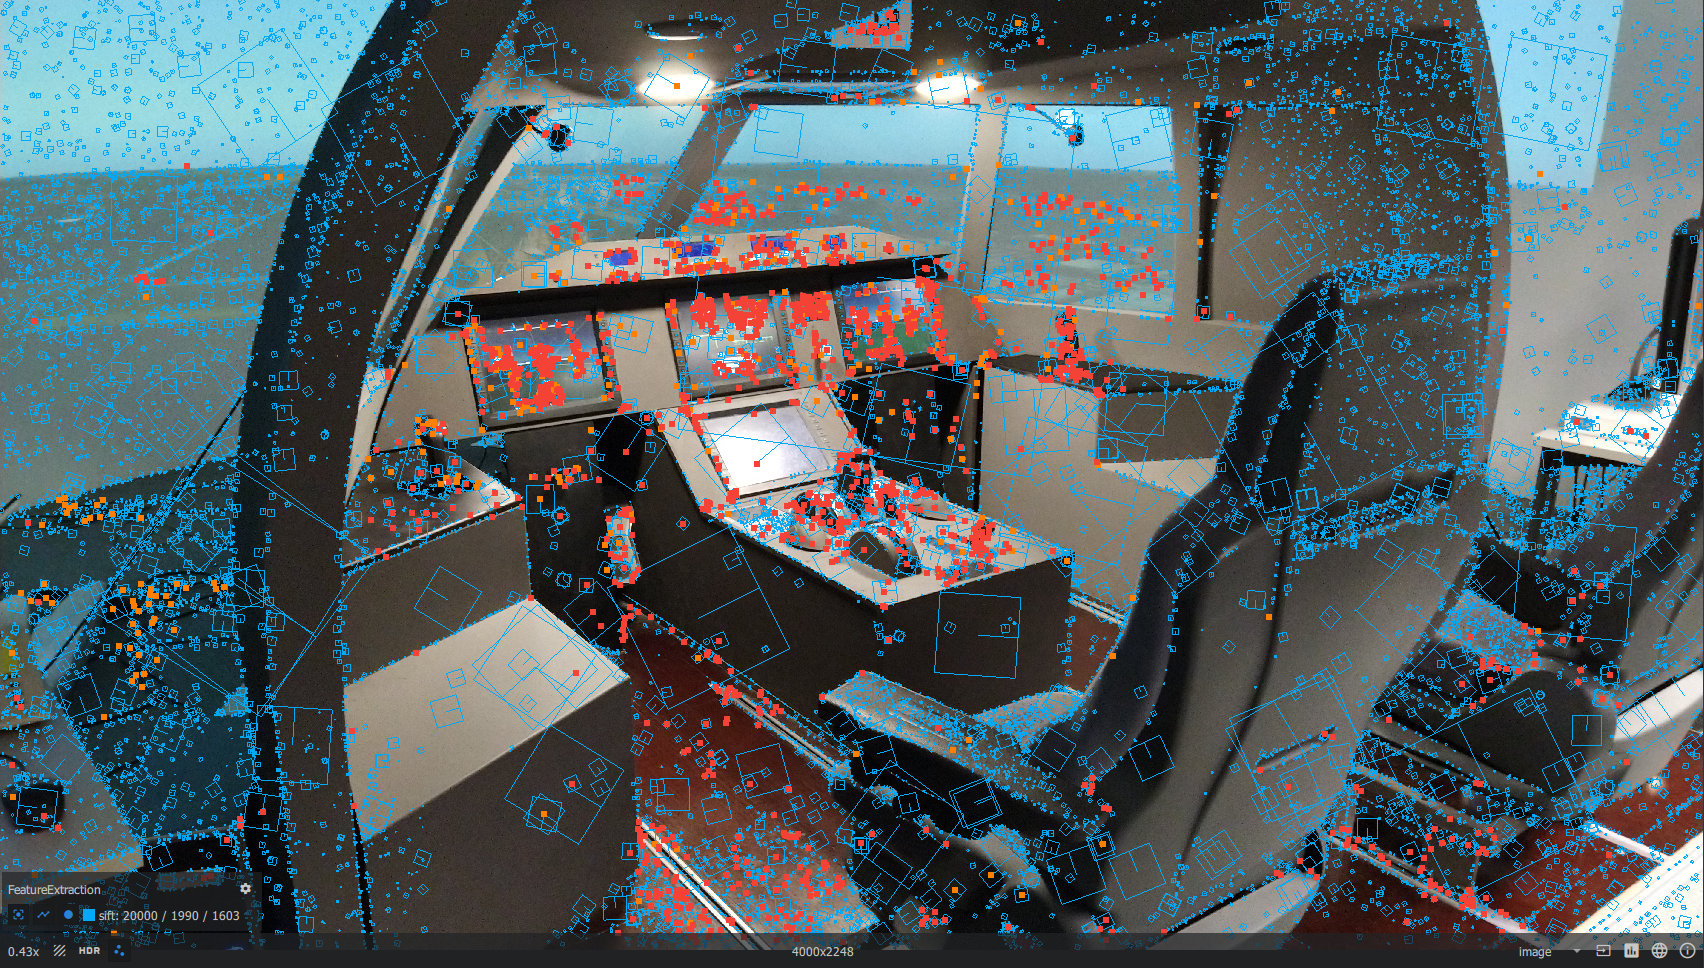
\includegraphics[width=0.8\textwidth]{meshroom-feature-extraction.png}
  \caption{One of the images processed by the photogrammetry pipeline. The features extracted by SIFT in the feature extraction step are highlighted in blue, the features matched with other pictures of the dataset are highlighted in orange. The points whose 3D position has been reconstructed in the structure from motion step are shown in red.}\label{fig:photogrammetry_feature_extraction_matching_reconstruction}
\end{figure}

\begin{figure}
  \centering
  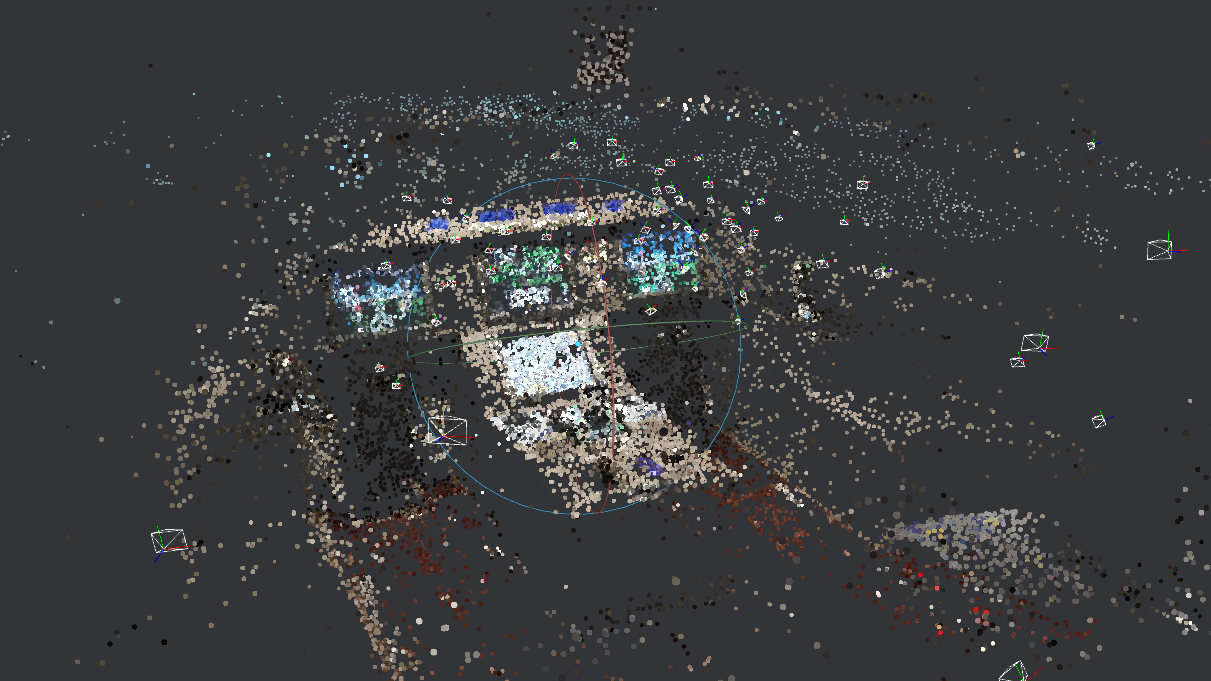
\includegraphics[width=0.8\textwidth]{meshroom-sparse.png}
  \caption{A view of the sparse reconstruction produced by Meshroom.}\label{fig:meshroom_sparse_reconstruction.png}
\end{figure}

This entire pipeline has been implemented in the open source software Meshroom\cite{alicevision_meshroom_nodate}, which makes it almost trivial to use this comparatively sophisticated approach. Around 130 pictures of the fixed-platform simulator in which \gls{holoassist} will be used were acquired with a phone camera and processed via Meshroom's photogrammetry pipeline implementation. Some of these images are shown in \autoref{fig:meshroom_rfs_pictures.png}. This yielded the final 3D-reconstructed mesh shown in \autoref{fig:meshroom_3d_reconstruction.png}. The result is quite remarkable, especially giving the poor lighting condition under which the pictures were acquired and the fact that the only required hardware is a phone camera. With some manual cleanup it is definitely sufficient to obtain an occlusion mesh for the simulator cockpit's shell, and with better pictures and/or a better pipeline implementation\cite{knapitsch_tanks_2017} it would be a perfect solution to the problem, satisfying all of the desired use cases.

\begin{figure}[p]
  \centering
  \subfloat{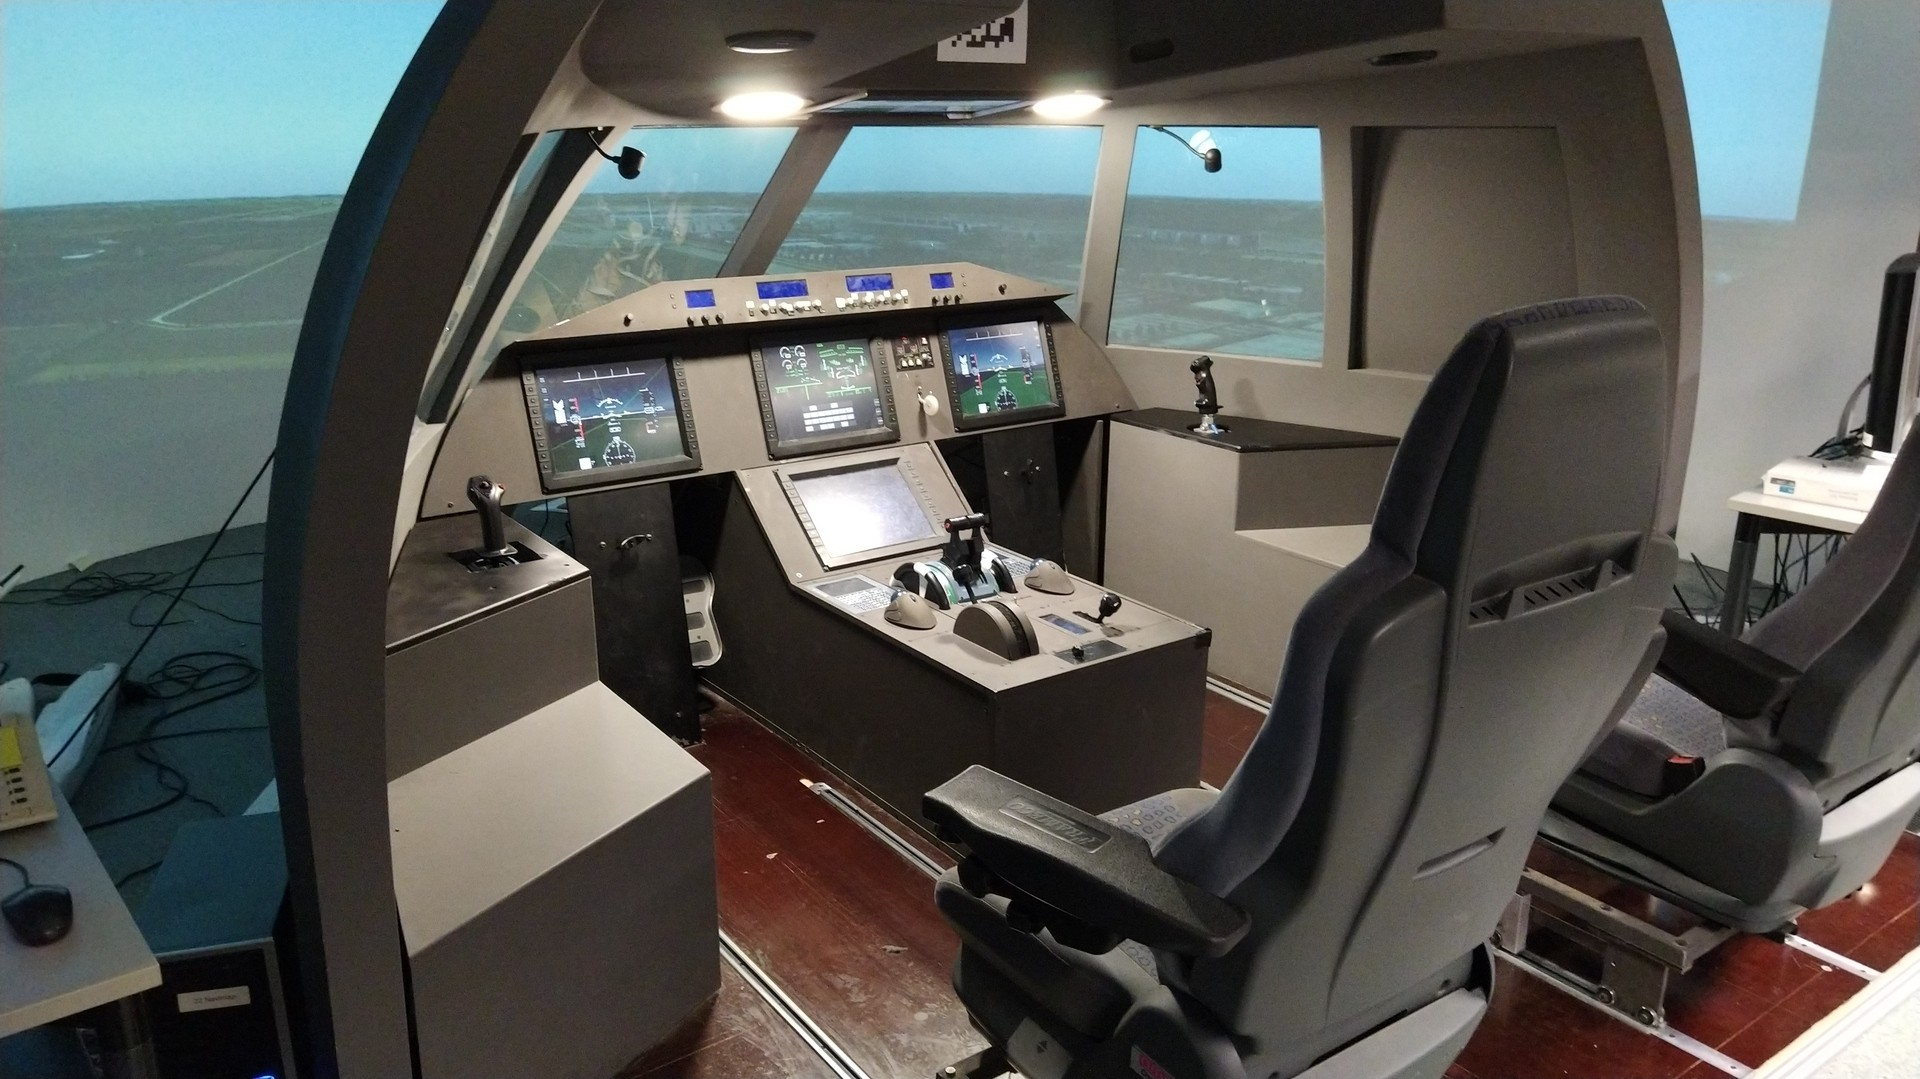
\includegraphics[height=0.27\textwidth]{photogrammetry-pic-1.jpg}}
  \hfill
  \subfloat{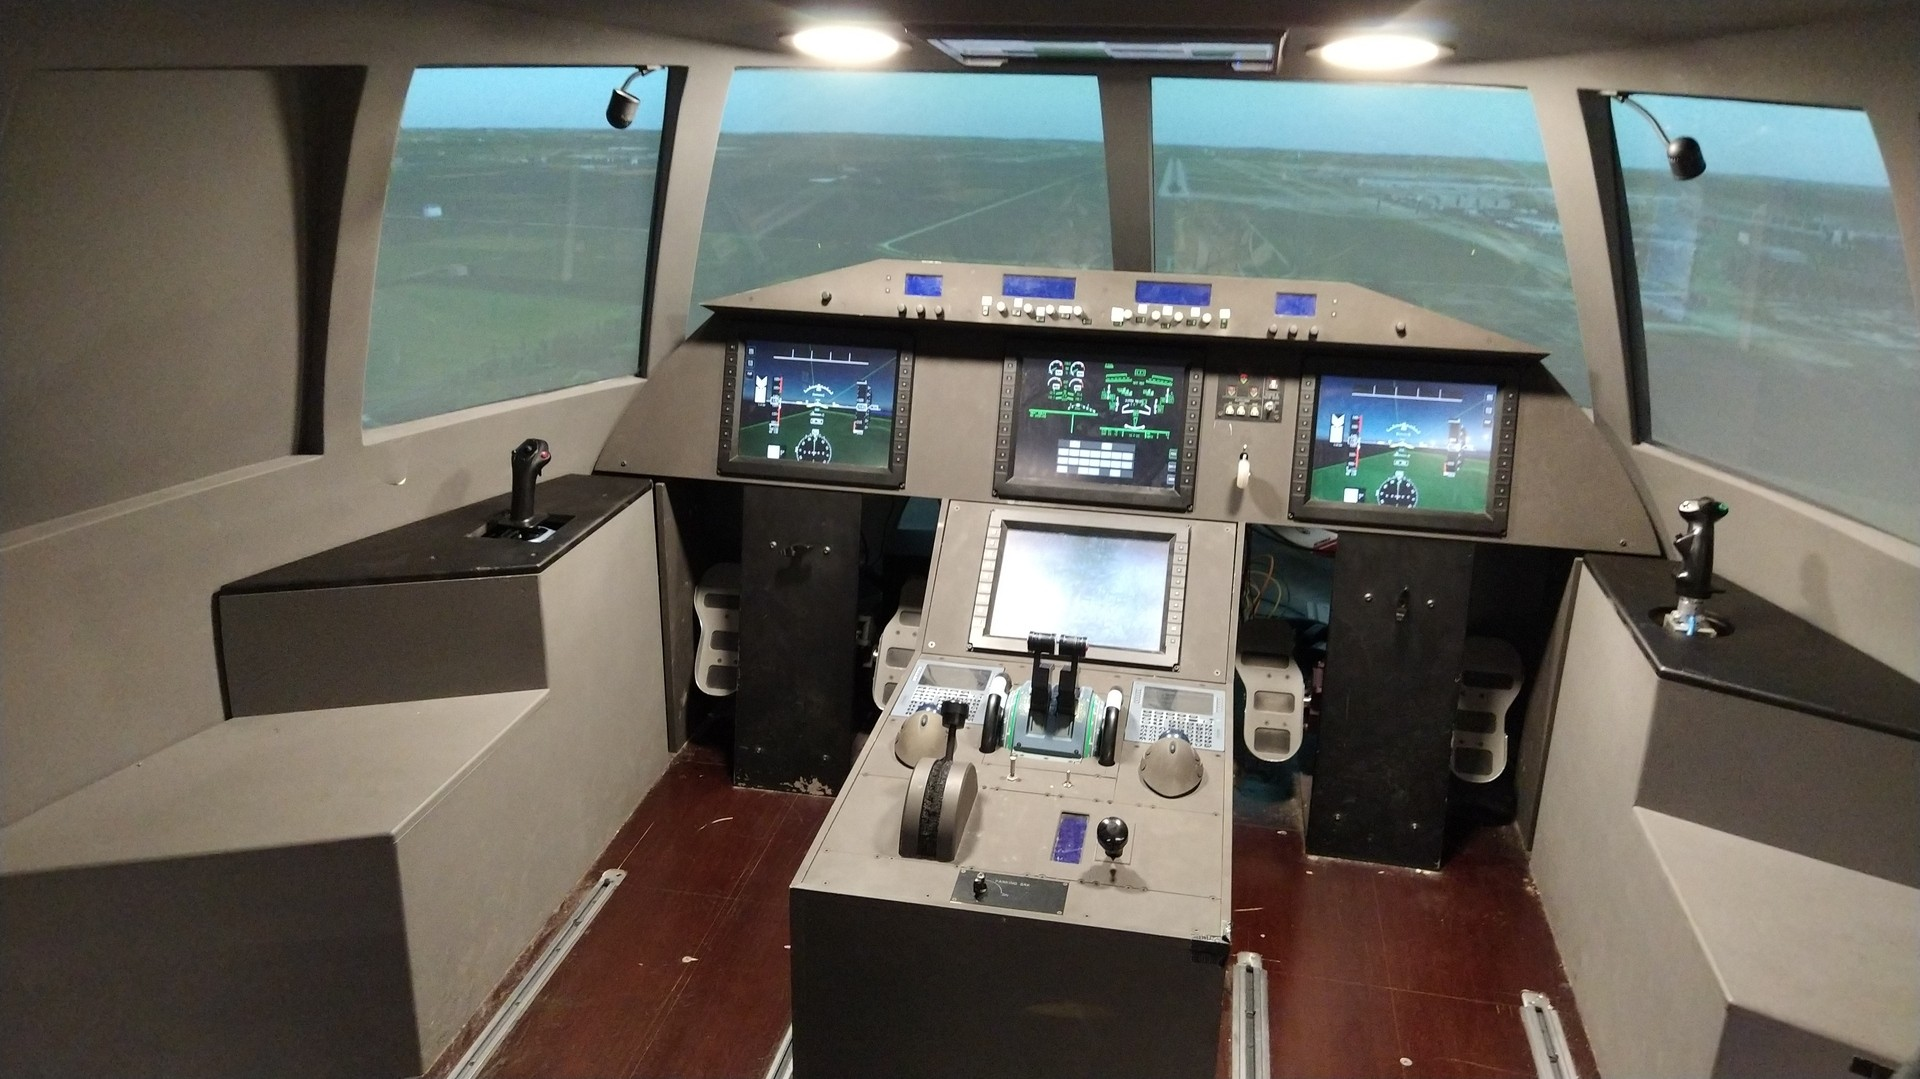
\includegraphics[height=0.27\textwidth]{photogrammetry-pic-2.jpg}}
  \caption{Two of the images used in the photogrammetry pipeline. As it can be seen, the images are relatively low-quality, as the lighting is not ideal, there are plenty of reflections and some of them had a bit of motion blur. Better images would most probably yield a better result, but this was sufficient for the test.}\label{fig:meshroom_rfs_pictures.png}
\end{figure}

\begin{figure}[p]
  \centering
  \subfloat{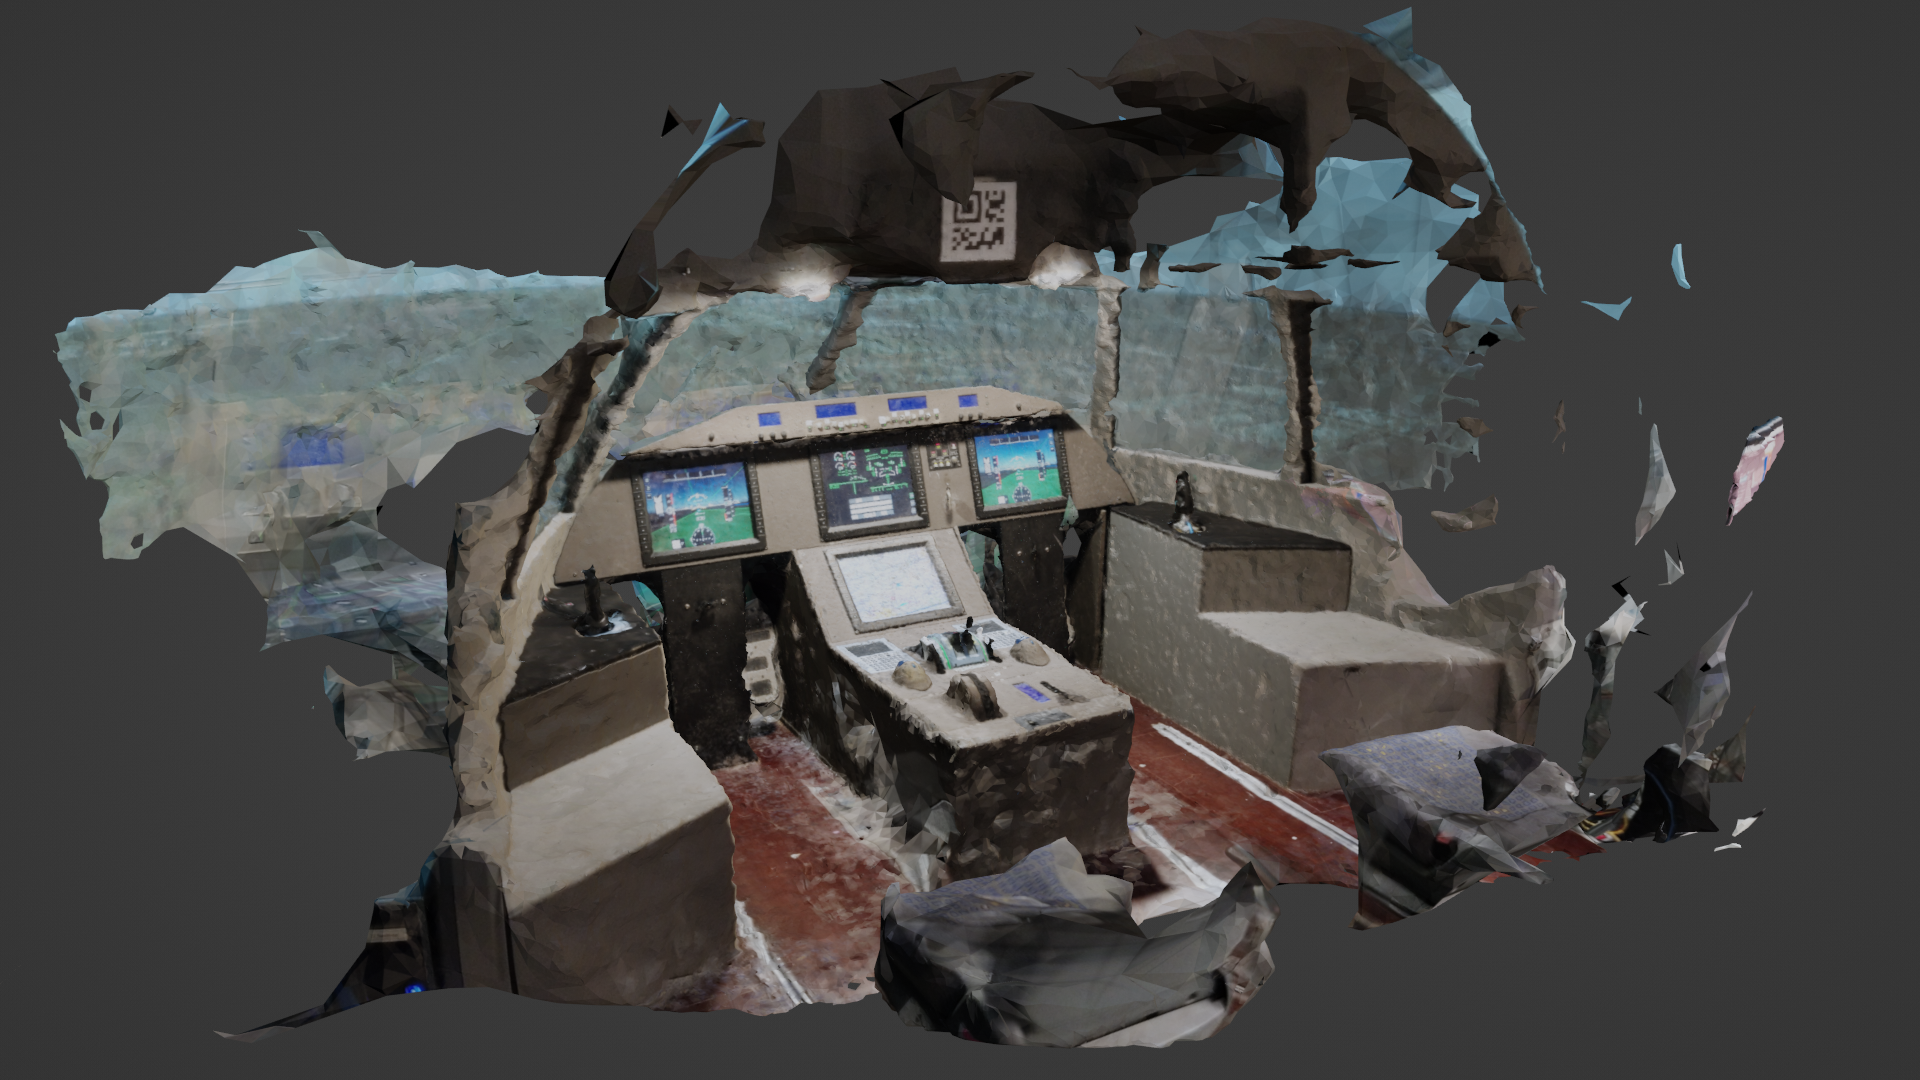
\includegraphics[height=0.27\textwidth]{meshroom-result-1.png}}
  \hfill
  \subfloat{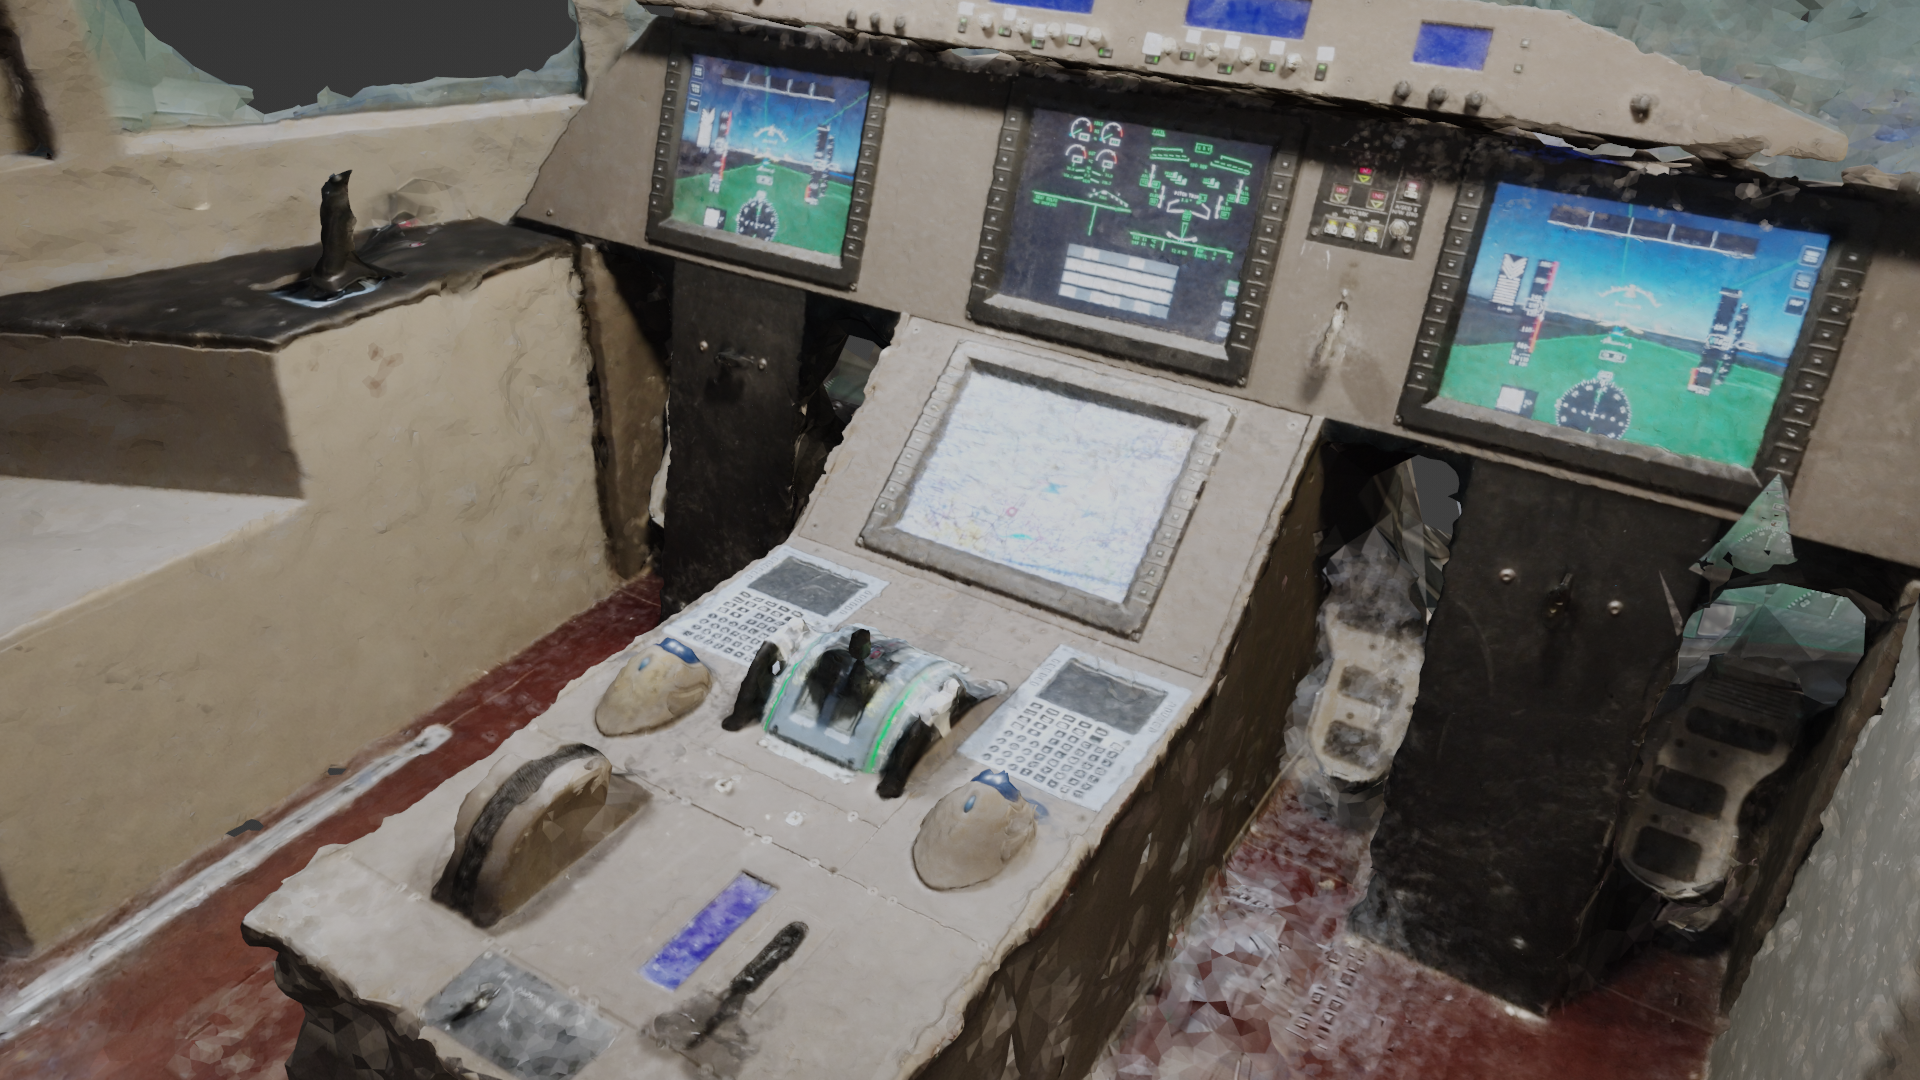
\includegraphics[height=0.27\textwidth]{meshroom-result-2.png}}
  \caption{The output of the Meshroom photogrammetry pipeline on the given image set. Despite the poor quality of the initial images, the result is more than acceptable.}\label{fig:meshroom_3d_reconstruction.png}
\end{figure}

\begin{figure}[p]
  \centering
  \subfloat{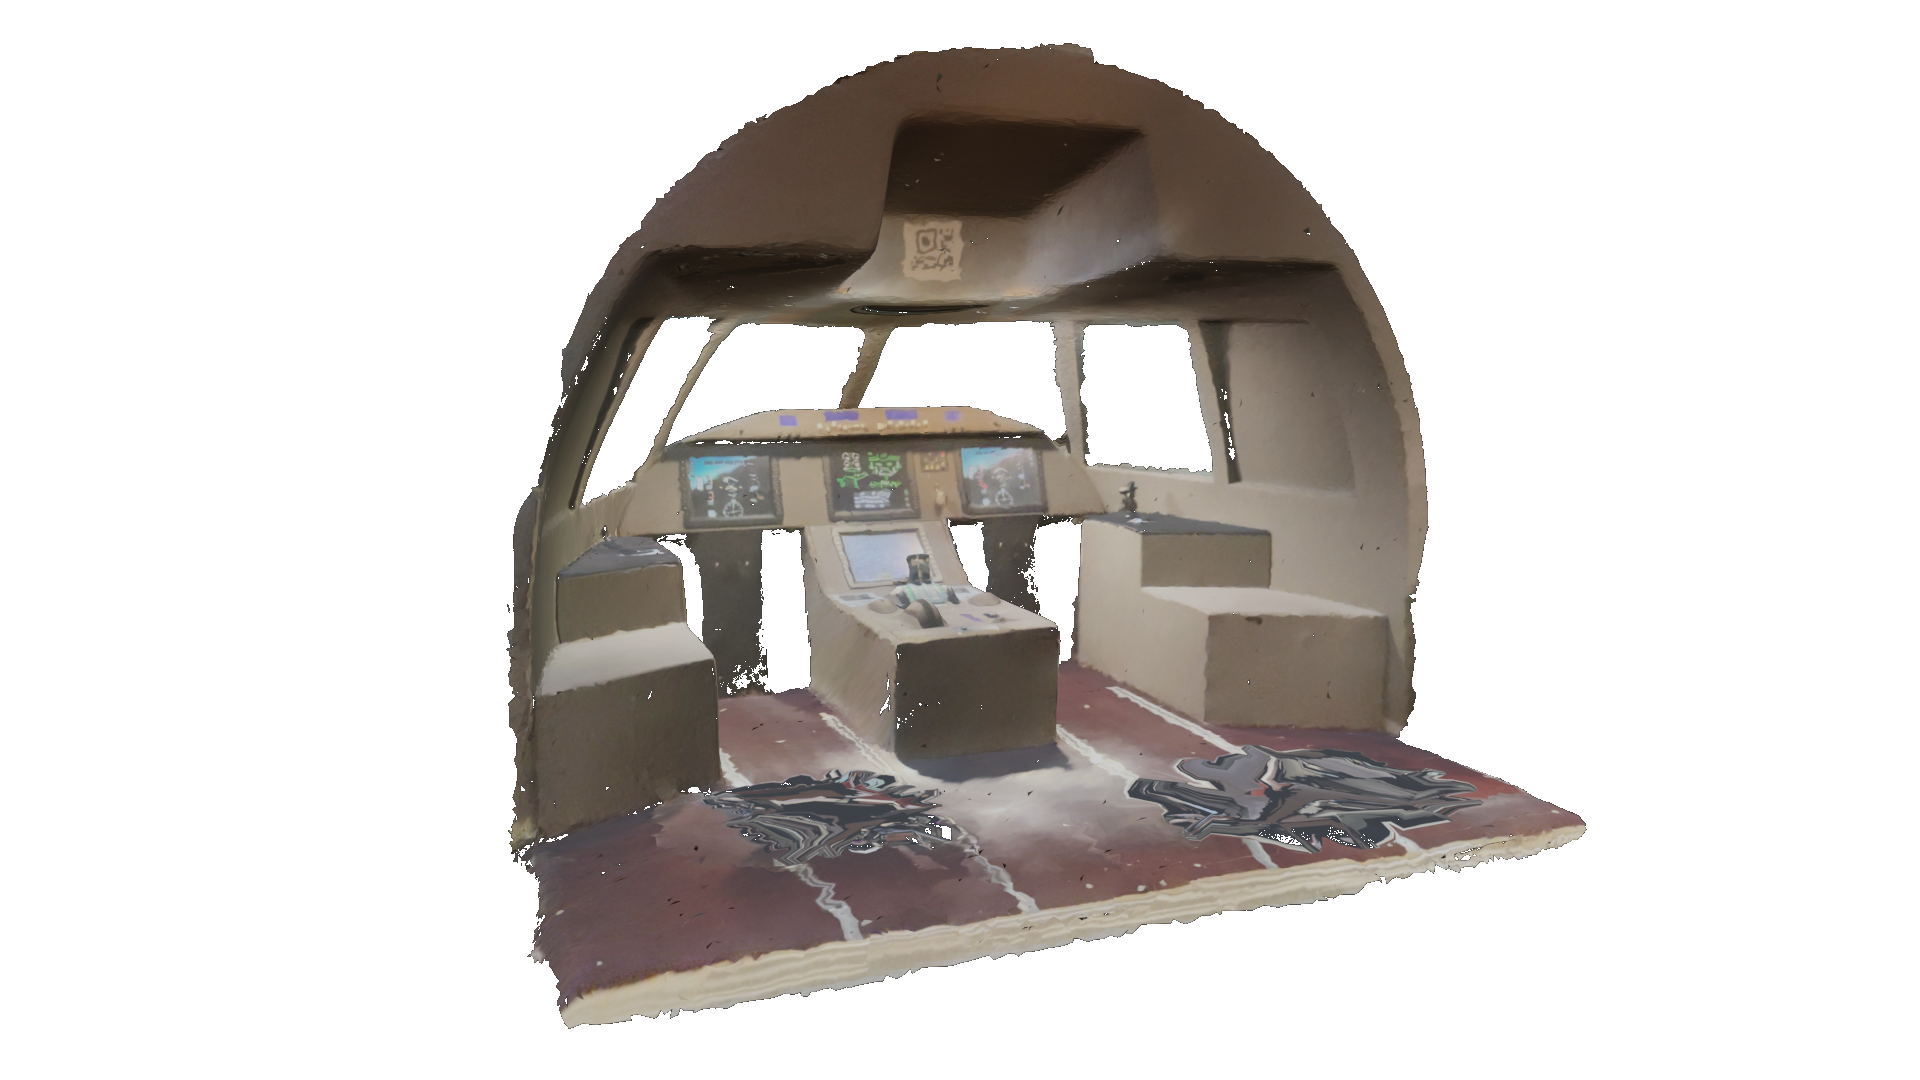
\includegraphics[height=0.27\textwidth]{final-3d-scan-1.png}}
  \hfill
  \subfloat{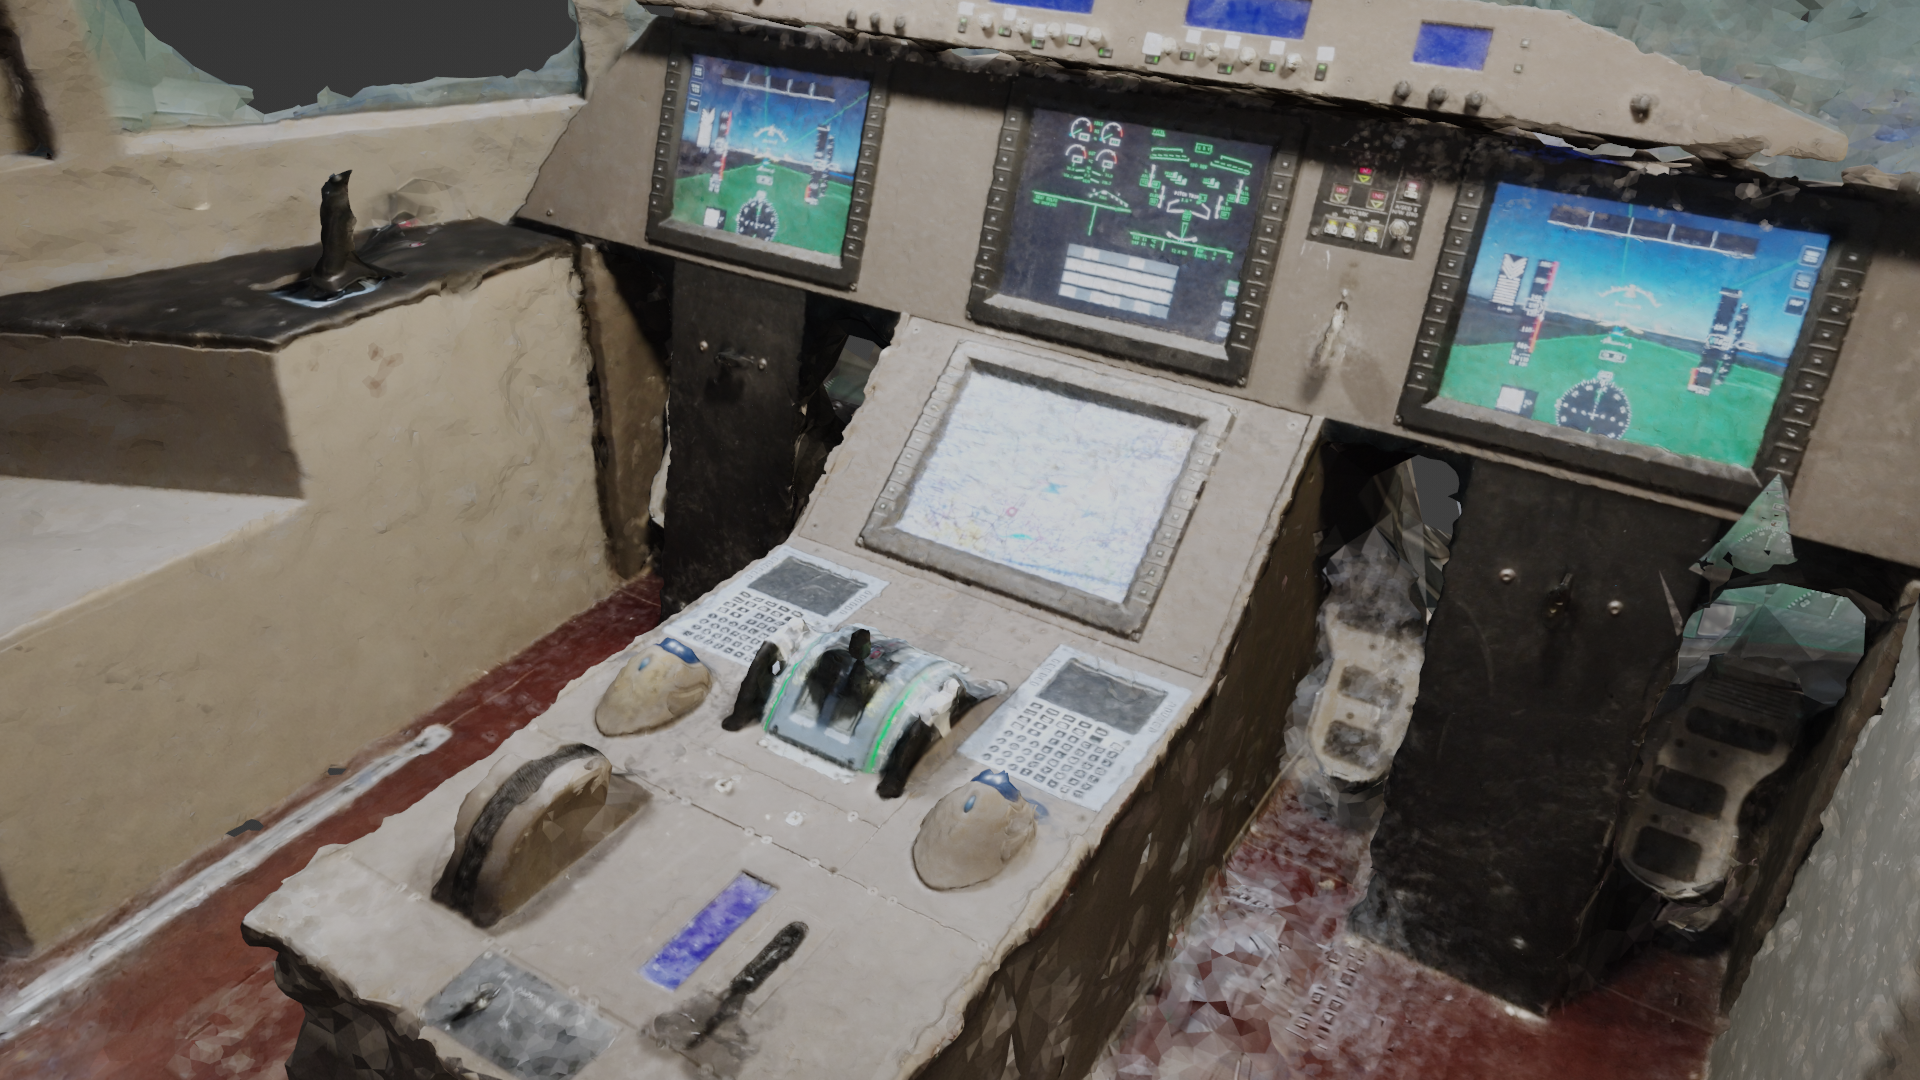
\includegraphics[height=0.27\textwidth]{meshroom-result-2.png}}
  \caption{The final 3D scan.}\label{fig:simulator_3d_scan.png}
\end{figure}

Another idea to acquire a digital double of the flight simulator comes from recent Apple iPads\cite{apple_inc_ipad_nodate}, which include a LIDAR sensor and an application that is able to use it to acquire a 3D scan of an environment. A quick attempt with this technology showed it to be superior than all of the other attempted approaches: the 3D scans it produces are precise and the texture that is generated for the 3D model allows to clearly distinguish also the positions of small-scale features like individual control knobs. Given the excellent results, it was decided to pause further investigation of photogrammetric techniques and utilize this approach instead.

Acquiring a full 3D scan of the simulator cockpit in a single step proved to be difficult: therefore, multiple different partially-overlapping 3D scans were independently acquired. However, these different meshes were not aligned: they were therefore imported in MeshLab\cite{cignoni_meshlab_2008} and aligned via its \gls{ICP} implementation\cite{zhang_fast_2021}. After the alignment, they were imported in Blender\cite{blender_foundation_blender_nodate}, where they were merged in a single mesh that could be used to handle the occlusion for \glspl{geofixedaug}. This also allowed some manual refinement, like the deletion of some unnecessary details (e.g.\ the pilot seats) and the automated simplification of the mesh to reduce its polygon count. This yielded the result shown in \autoref{fig:simulator_3d_scan.png}. This mesh was then imported in Unity, where it was positioned in roughly the correct place with respect to the \texttt{GameObject}s acting as space pins (and therefore to what will be the QR codes positions in the real world). This rough positioning was obtained by measuring the real world offset between the QR codes and a particular point of the simulator cockpit shell with a tape measure and then replicating that offset in the Unity world between the space pins and the matching point on the simulator digital double. A further manual refinement was then performed by running the application on the Hololens and using the \gls{remoteunityeditor} (see \autoref{section:developerutilities}) to move the digital double until the overlap between it and the real simulator was visually satisfying. The resulting virtual position of the digital double was then integrated in the Unity project to be the default one by using the same simulator-specific JSON file in which the virtual positions of the space pins are defined. For the simulator in which \gls{holoassist} was tested this looks like \autoref{lst:sim_digita_double_virtual_positions_json}.

\begin{figure}[t]
  \centering
  \begin{tabular}{c}
  \begin{lstlisting}[language=json]
    {
        "planeMesh": [ 0.6909984, -1.27500093, 0.3499981],
        "spacePins": {
            // all the space-pins locations
        },
        // other simulator-related information not relevant here
    }
  \end{lstlisting}
  \end{tabular}
  \caption{An extract of the JSON file that describes the virtual positions of the simulator digital double.}\label{lst:sim_digita_double_virtual_positions_json}
\end{figure}

\begin{figure}[t]
  \centering
  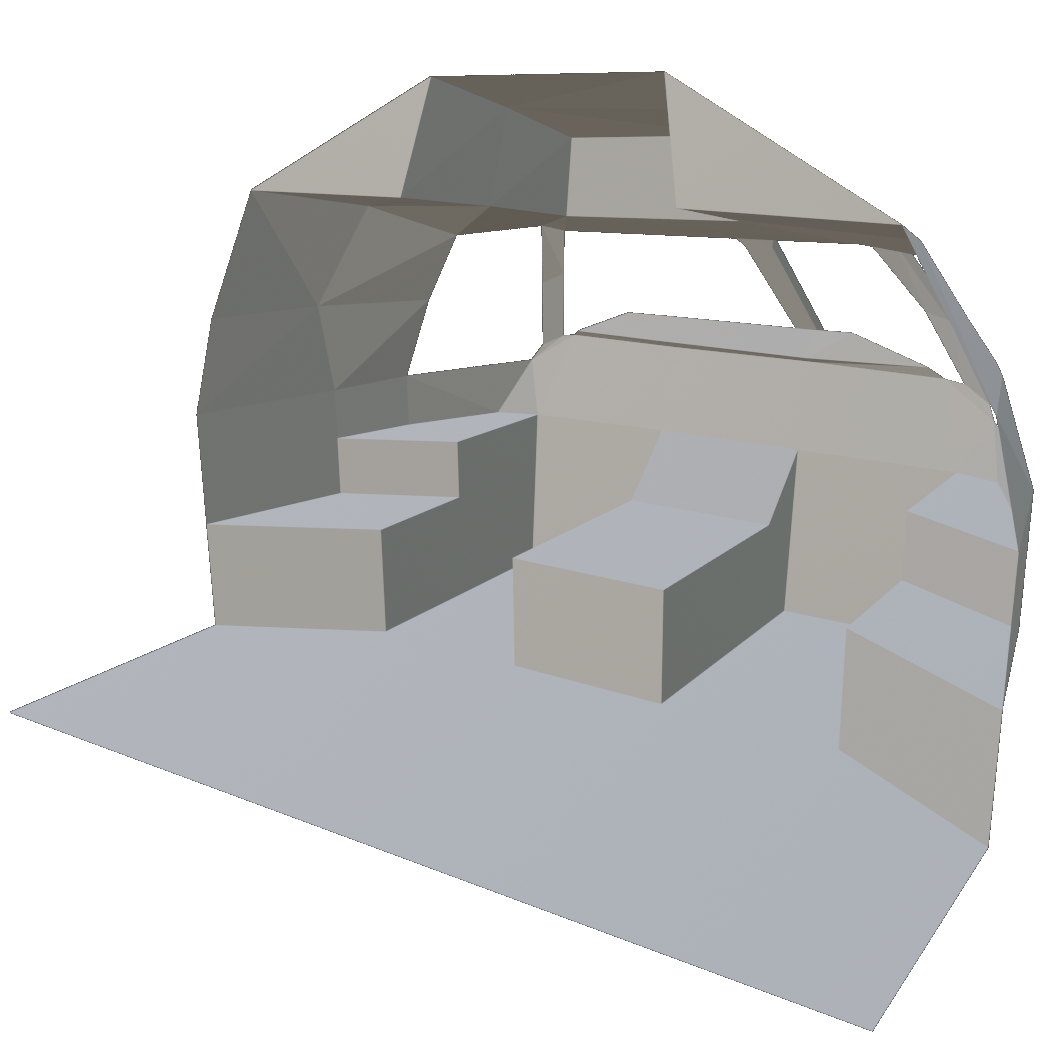
\includegraphics[width=0.4\textwidth]{actual-plane-mesh.png}
  \caption{The extremely low-polygonal mesh that is actually used as occlusion mesh on the Hololens.}\label{fig:actual_simulator_mesh.png}
\end{figure}

In conclusion, \gls{holoassist} is now able to place in the virtual world a digital double of the simulator cockpit's shell such that it is correctly aligned with the real one to provide the occlusion required for \glspl{geofixedaug}. Additionally, the acquired 3D scan is precise enough to help designing \glspl{planefixedaug}. Moreover, two easily accessible ways of acquiring the digital double were discovered, improving the workflow based on traditional \gls{CAD}-based approach. Another advantage of these two approaches is that their complexity is irrespective of how intricate the simulator's shape is, whereas it is instead more difficult to design a \gls{CAD} model for a more complex shape.

A final footnote should however be made. The mesh resulting from the 3D scan, despite the simplification done in Blender, still has a decent polygonal count (around 9000 triangles). Given the limited computational budget of the Hololens and the fact that the occlusion mesh does not need to be extremely detailed, it was decided to use the 3D scanned mesh to draw a simplified occlusion mesh that only captures the essential details, as shown in \autoref{fig:actual_simulator_mesh.png}. This resulted in a significantly lighter mesh (around 200 triangles) which is still able to provide the required occlusion. Nevertheless, having the 3D scanned mesh allowed to create this simplified mesh very quickly, as it could be used as a reference without having to obtain any real-world measurement.

\section{Geo-fixed augmentations}\label{section:geofixedaugmentations}

At this point, \gls{holoassist} contains the foundations that are required to start working on actually displaying \gls{geofixedaug}, which are augmentations that appear to be placed at a specific geographical point when looking outside the windows of the simulator cockpit.

\subsection{Geodesy fundamentals}\label{section:geodesyfundamentals}
Understanding how \glspl{geofixedaug} are represented and how their rendering process works requires some familiarity with some geodesy fundamentals.

A point on the Earth can be identified precisely in different ways known as \glspl{CRS}. Different \glspl{CRS} offer different tradeoffs (e.g.\ regarding precision vs.\ area of applicability) and use different parameters to represent points. The EPSG Geodetic Parameter Dataset\cite{iogp_geomatics_committee_epsg_nodate} keeps track of the different \glspl{CRS} and assigns an identifier to every one of them.

One of the most commonly known \glspl{CRS} is EPSG:4326, which approximates the Earth surface with well-defined ellipsoid known as the WGS84 datum surface\cite{noauthor_epsg4326_nodate}. The ellipsoid's center is the Earth's center of mass and it has an equatorial radius (major semi-axis) of $a = 6378137$m and a flattening $f = 1 / 298.257223563$, leading to a computed semi-minor axis $b = 6356752.3142$m\cite{zintl_design_2020}. The resulting shape is shown in \autoref{fig:epsg4979_example_point.png}. In this \gls{CRS} a point on the Earth surface is identified by two numbers known as latitude and longitude: they describe, respectively, the angle between the equatorial plane and the point to be described and the angle between the IERS Reference Meridian (colloquially known as \enquote{the Greenwhich meridian}) and the point to be described. A commonly used extension of this \gls{CRS} is \gls{epsg4979}, which adds a third coordinate, \enquote{height}, to measure the distance between the point to be described and the ellipsoid along the ellipsoid's normal at that point. An example of a point in this \gls{CRS} is shown in picture \autoref{fig:epsg4979_example_point.png}.

\begin{figure}
  \centering
  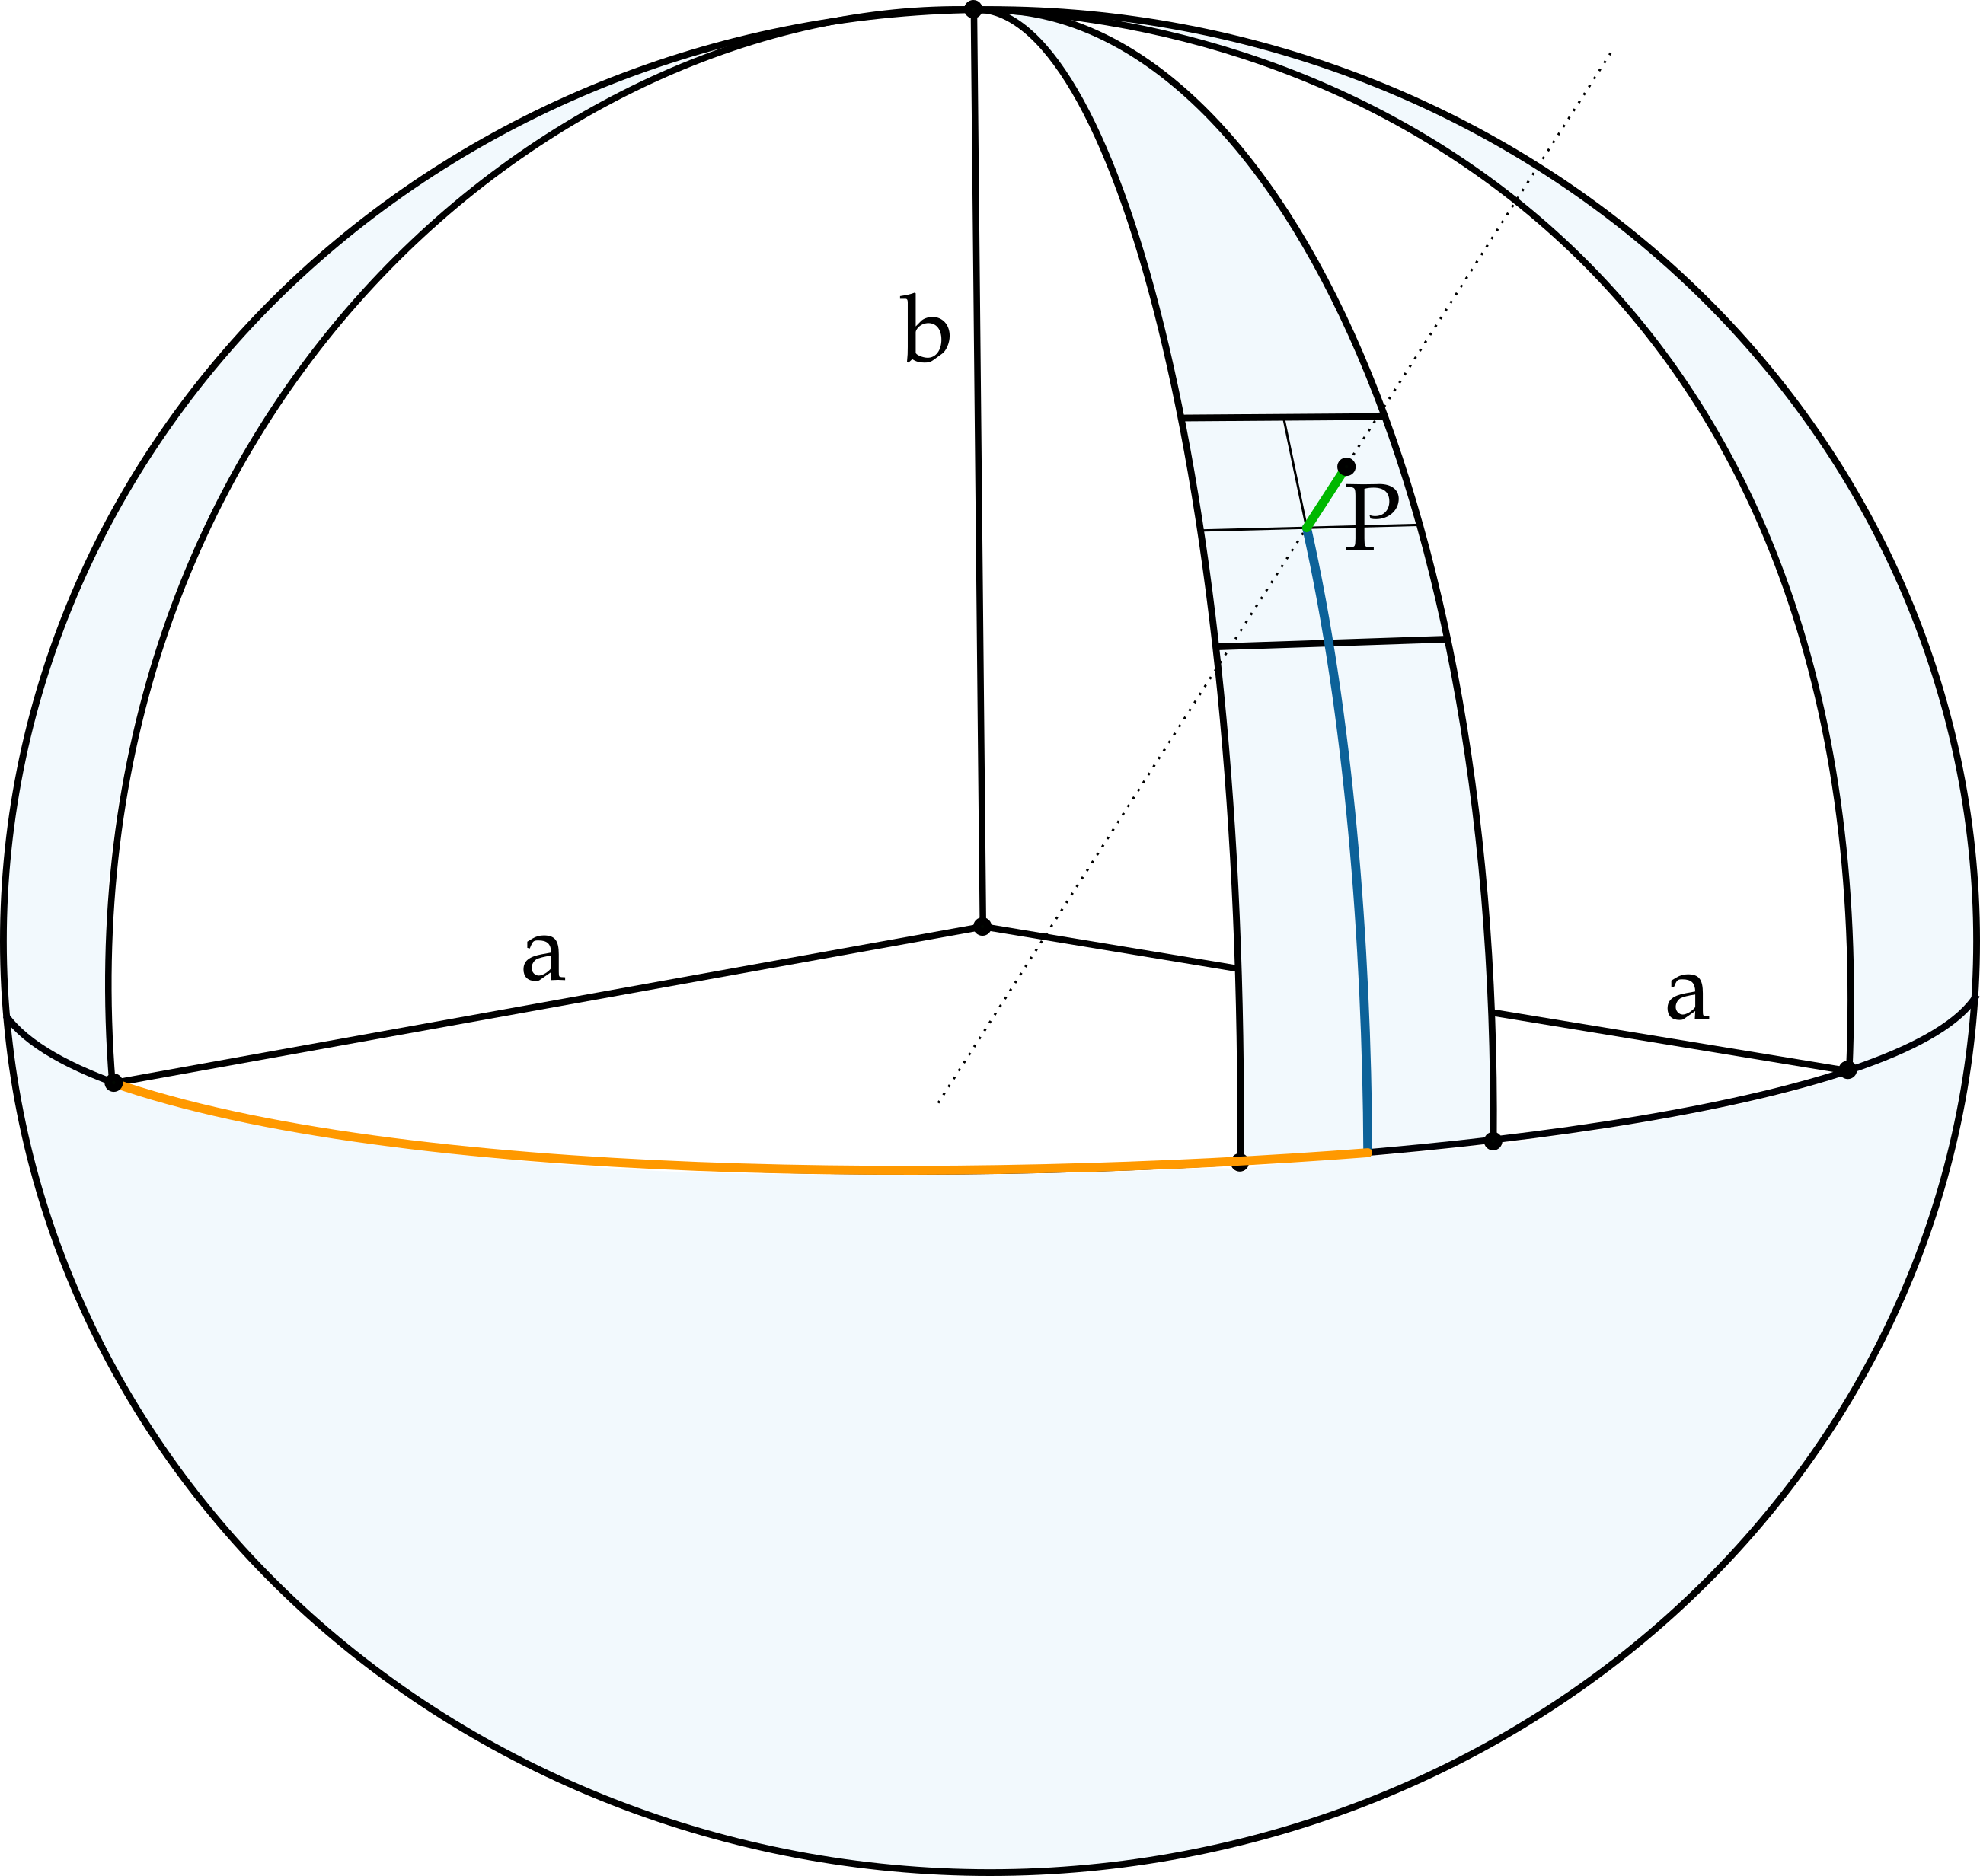
\includegraphics[width=0.5\textwidth]{wgs-point.png}
  \caption{The light-blue shape shows a depiction of the WGS84 datum surface: it is an oblate spheroid with $a$ as the major semi-axis and $b$ as the minor semi-axis. $P$ represents a point in the \gls{epsg4979} \gls{CRS}. The longitude of $P$ is the angle implied by the orange arc, its latitude is the angle implied by the blue arc and its height is the length of the green segment. It should be noted that the height is computed along the normal to the ellipsoid surface at point $P$ (the dotted line), which does not necessarily intersect the ellipsoid center.}\label{fig:epsg4979_example_point.png}
\end{figure}

\begin{figure}
  \centering
  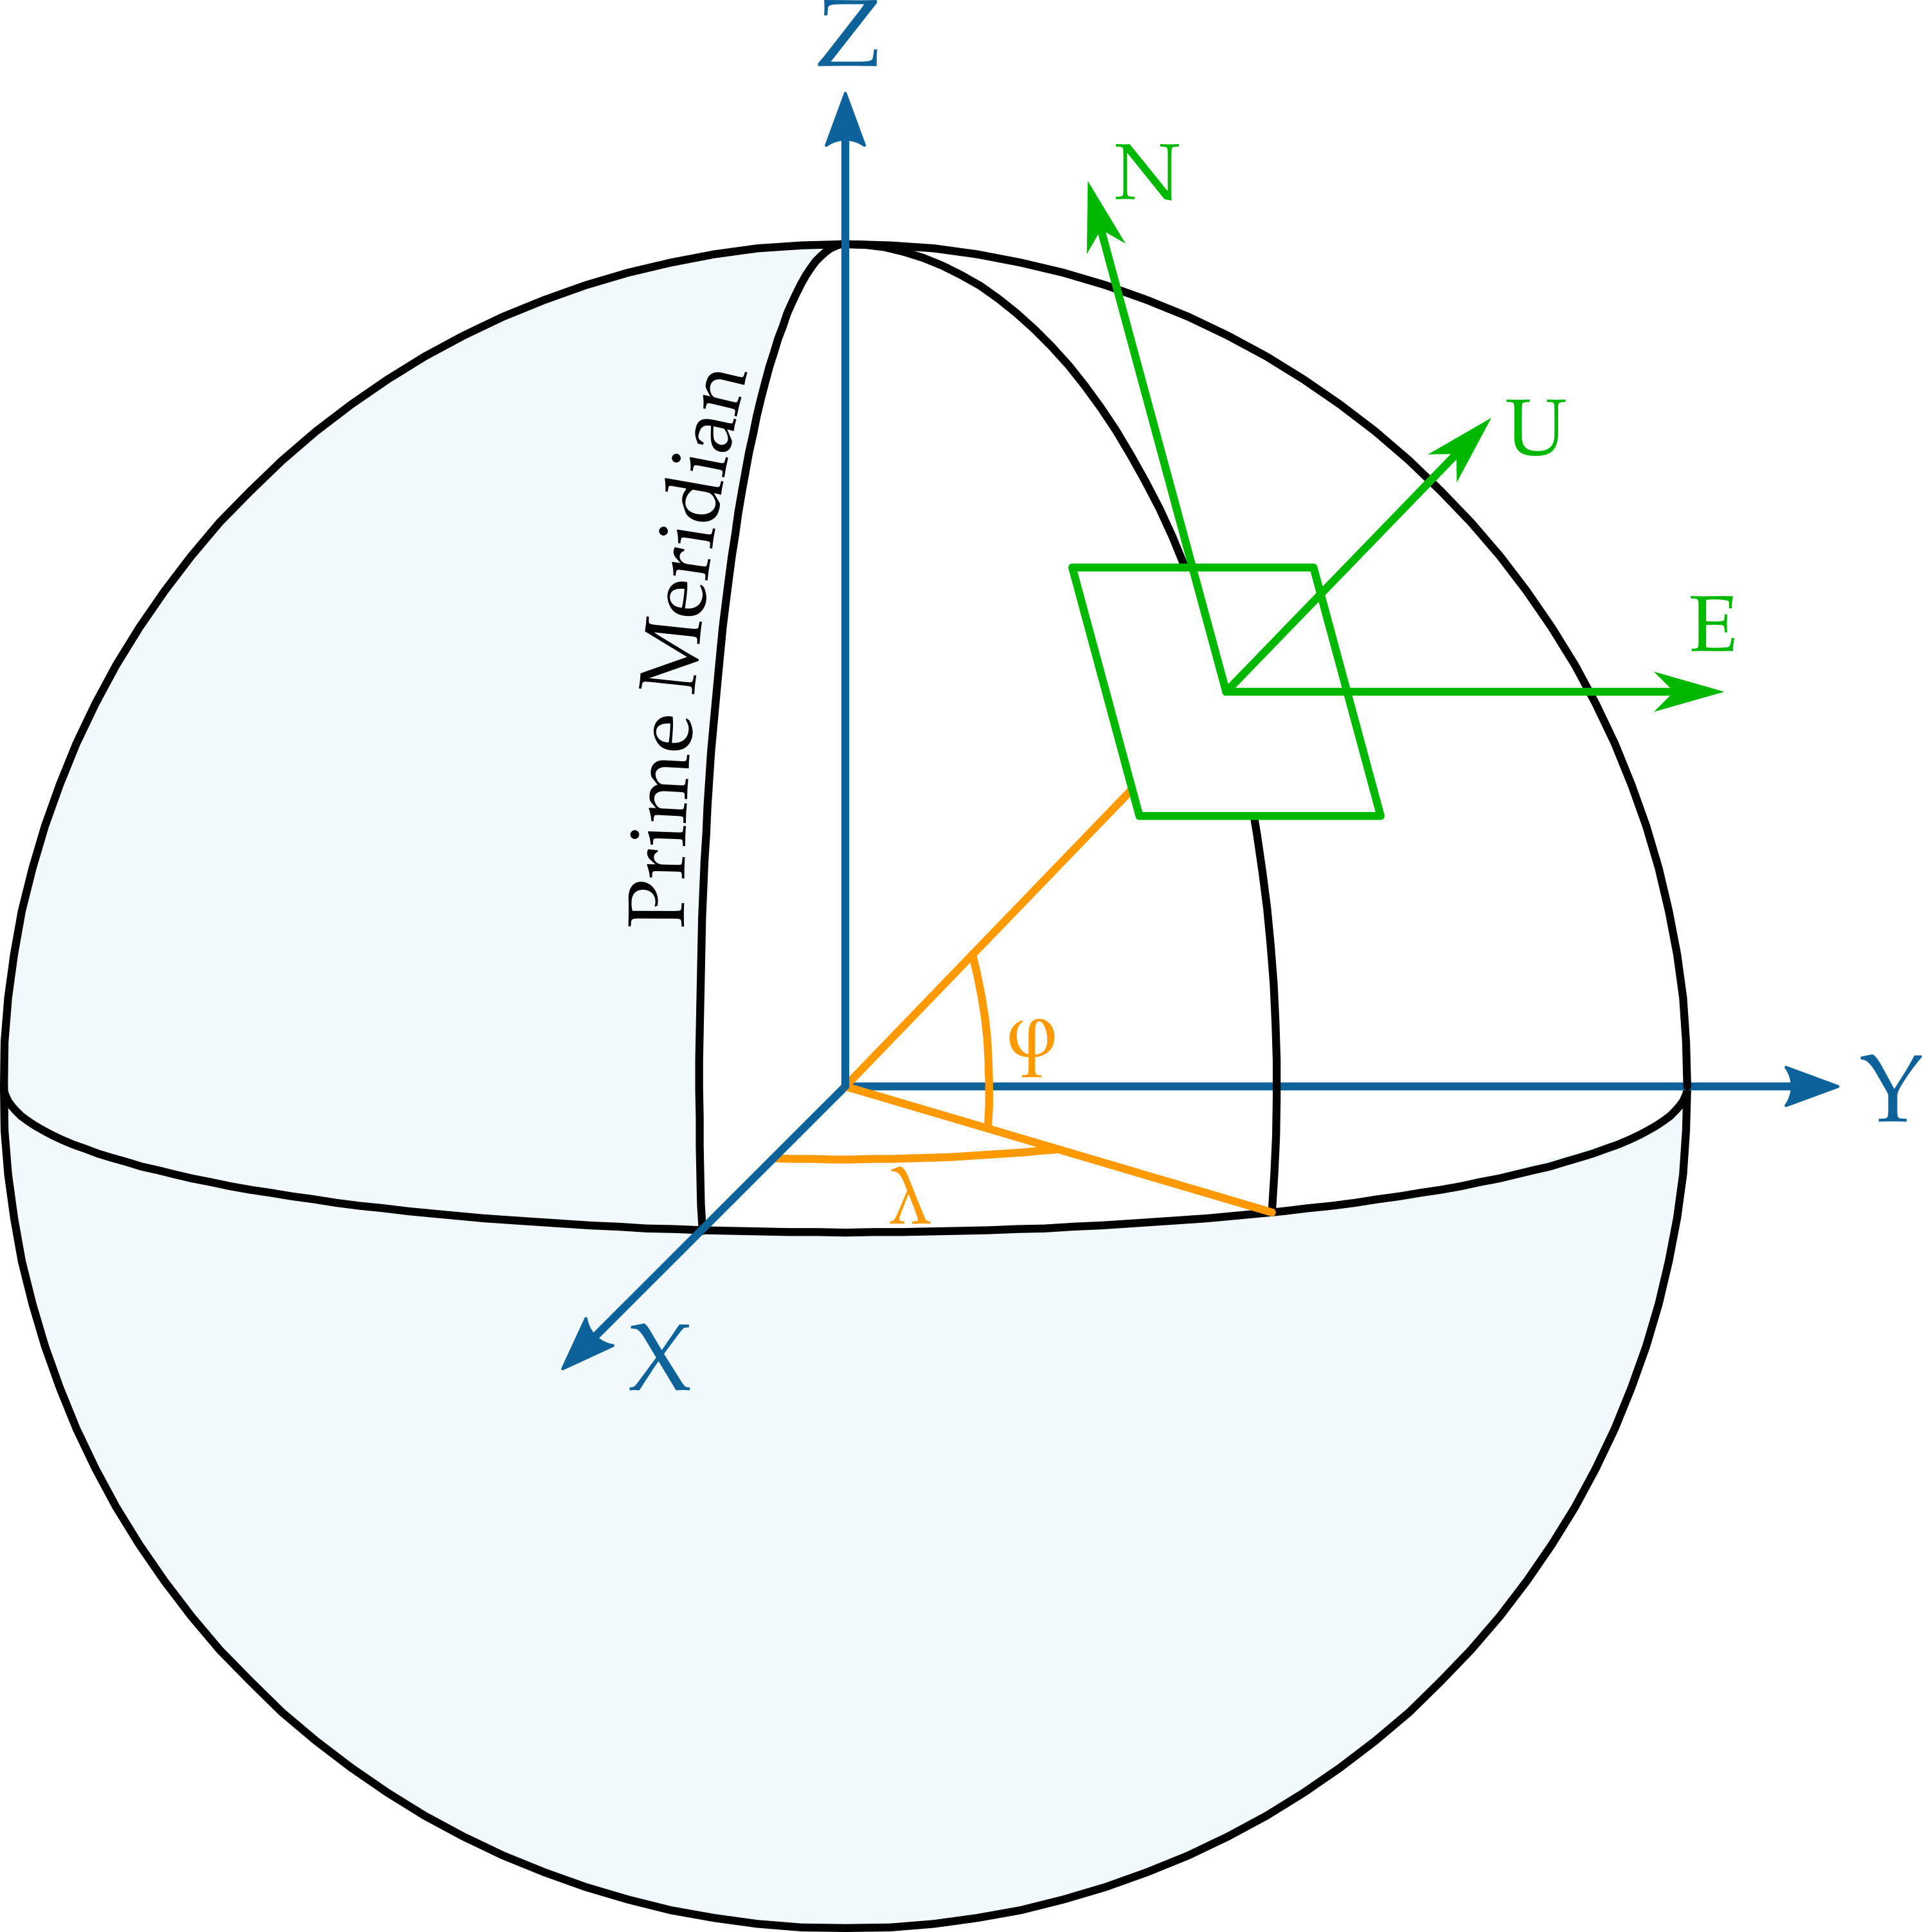
\includegraphics[width=0.5\textwidth]{topocentric-crs.png}
  \caption{A visual representation of a \gls{ENU} topocentric \gls{CRS} and its relationship with the \gls{epsg4978} \gls{CRS}. Original image from Wikipedia\cite{noauthor_local_2022}.}\label{fig:topocentric_crs_example.png}
\end{figure}

However, \gls{epsg4979} does not use an Euclidean space, and this complicates some computations. Therefore, another \gls{CRS} often used is \gls{epsg4978}, which instead \emph{is} an Euclidean space. It is an \gls{ECEF} coordinate system whose origin is at the center of the WGS84 ellipsoid. In this \gls{CRS}, a point is represented by a triplet of numbers denoting the distance from the origin in meters along each of the three axes, respectively known as X axis, Y axis and Z axis. The X axis is on the equatorial plane and intersects the IERS Reference Meridian, while the Z-axis is parallel to the mean earth rotation axis. As \gls{epsg4978} is the only \gls{ECEF} \gls{CRS} used in this document, the terms \gls{ECEF} and \gls{epsg4978} will be used interchangeably.

The last type of \gls{CRS} that needs to be discussed is actually a class of \glspl{CRS} known as topocentric \acrlongpl{CRS}. An example of such system is EPSG:5819. These \glspl{CRS} define a plane that is tangent to the Earth's ellipsoidal surface at a specific location called \enquote{topocentric origin}. This location is then used to define a Cartesian frame centered at it, with two axes lying on the tangent plane and the third one parallel to the normal of the plane. A visual depiction of this kind of \gls{CRS} is shown in \autoref{fig:topocentric_crs_example.png}. \gls{holoassist} uses a type of topocentric \glspl{CRS} known as \gls{ENU}, which is a right-handed coordinate system in which one axis points towards the north pole, one points \enquote{away} from the ellipsoid surface (along the plane normal) and the third one is perpendicular to these two, which means it points \enquote{east}. An \gls{ENU} \gls{CRS} offers two main advantages with respect to an \gls{ECEF} \gls{CRS}: it is more intuitive to use in the context of the position of an aircraft and its coordinates are smaller in absolute value, leading to fewer numerical precision issues during computations. However, it is a flat approximation of the Earth surface around a point, and is therefore accurate only in proximity of the topocentric origin.

\Gls{holoassist} also needs to be able to take points expressed in one \gls{CRS} and convert them to another. Fortunately, conversion procedures between common EPSG \gls{CRS} are well-known and often already implemented in geodesy libraries (like PyProj\cite{noauthor_pyproj_nodate}) and tools (like QGis\cite{qgis_development_team_qgis_nodate}). In the interest of producing a self-contained document, the conversion procedures between the \glspl{CRS} used by \gls{holoassist} have been sourced from the literature\cite{zintl_design_2020} and reported here without proof.

First of all, \gls{holoassist} needs to be able to convert between \gls{epsg4979} and \gls{epsg4978}. Given the parameters of the WGS84 datum:

\begin{IEEEeqnarray}{rCl}
    a & = & 6378137m \\
    b & = & 6356752.3142m \\
    f & = & \frac{a - b}{a} \\
    e & = & \sqrt{f(2 - f)}
\end{IEEEeqnarray}

The radius of curvature in the prime vertical of the WGS84 ellipsoid at a particular latitude $\varphi$ can be computed as follows:

\begin{equation}
    N\left(\varphi\right) = \frac{a}{\sqrt{1 - e^2 \sin^2 \varphi}}
\end{equation}

Given a point $\mathbf{p}_{\text{\glsentrytext{epsg4979}}} = (\text{latitude}, \text{longitude}, \text{altitude})^T = (\varphi_p, \lambda_p, h_p)^T$ in the \gls{epsg4979} \gls{CRS}, it can be converted to \gls{ECEF} with the following function:
\begin{IEEEeqnarray}{rCl}
    \label{eq:convertEPSG4979toECEF}
    \mathbf{p}_{\text{ECEF}} & = & \convertWGStoECEF{\mathbf{p}_{\text{EPSG:4979}}} \\
    & = & \begin{pmatrix}
        \left(N + h_p \right)\cos\varphi_p\cos\lambda_p\\
        \left(N + h_p \right)\cos\varphi_p\sin\lambda_p\\
        \left(\left(1 - e^2\right) N + h_p\right) \sin\varphi_p\\
    \end{pmatrix}
\end{IEEEeqnarray}

The other conversion that \gls{holoassist} needs to be able to do is from \gls{epsg4978} to a topocentric \gls{ENU} \gls{CRS} and vice versa. Let $\mathbf{o} = (\varphi_o, \lambda_o, h_o)$ be an \gls{epsg4979} point describing the topocentric origin of the destination \gls{ENU} system and $\mathbf{p}_{\text{ECEF}}$ be the \gls{epsg4978} point that we want to convert. Moreover, let:
\begin{equation}
\mathbf{o}_{\text{ECEF}} = \convertWGStoECEF{\mathbf{o}}
\end{equation}
Then the desired conversion is:
\begin{IEEEeqnarray}{rCl}
    \label{eq:convertECEFtoENU}
    \mathbf{p}_{\text{ENU}} & = & \convertECEFtoENU{\mathbf{p}_{\text{ECEF}}}{\mathbf{o}} \\
    & = & \begin{pmatrix}
        -\sin\lambda_o & \cos\lambda_o & 0 \\
        -\sin\varphi_o \cos\lambda_o & -\sin\varphi_o \sin\lambda_o & \cos \varphi_o \\
        \cos\varphi_o\cos\lambda_o & \cos\varphi_o\sin\lambda_o & \sin\varphi_o
    \end{pmatrix} \left(\mathbf{p}_{\text{ECEF}} - \mathbf{o}_{\text{ECEF}}\right)
\end{IEEEeqnarray}

This conversion can be straightforwardly inverted to obtain the function $\convertENUtoECEF{\mathbf{p}_{\text{ENU}}}{\mathbf{o}}$, which converts a point from an \gls{ENU} system with topographic origin $\mathbf{o}$ to the \gls{ECEF} \gls{CRS}:
\begin{IEEEeqnarray}{rCl}
    \label{eq:convertENUtoECEF}
    \mathbf{p}_{\text{ECEF}} & = & \convertENUtoECEF{\mathbf{p}_{\text{ENU}}}{\mathbf{o}} \\
    & = & \mathbf{o}_{\text{ECEF}} + \begin{pmatrix}
        -\sin\lambda_o & \cos\lambda_o & 0 \\
        -\sin\varphi_o \cos\lambda_o & -\sin\varphi_o \sin\lambda_o & \cos \varphi_o \\
        \cos\varphi_o\cos\lambda_o & \cos\varphi_o\sin\lambda_o & \sin\varphi_o
    \end{pmatrix}^T \mathbf{p}_{\text{ENU}}
\end{IEEEeqnarray}


\subsection{Geo-fixed augmentations representation}\label{sec:geofixedaug_representation}

A good starting point is to determine the best way to represent this kind of augmentations: regardless of how \gls{holoassist} will handle them internally, it is desirable to expose to the \gls{API}'s users a straightforward and easy to use representation which at the same time maintains as much flexibility as possible.

Usually, computer graphics applications represent 3D meshes as a set of triangles, encoded with two lists:

\begin{enumerate}
    \item A list of vertices, containing the 3D coordinates of the vertices of all the triangles;
    \item And a list of indices, in which every elements points to an item of the list of vertices. Starting from the beginning of this list, each triplet of elements describes a triangle of the mesh.
\end{enumerate}

This representation is preferred because the same vertex is usually part of multiple triangles: therefore, storing its coordinates only once allows to save memory. Since this representation is so ubiquitous and flexible, it was used as a starting point to design \gls{holoassist}'s interface.

\gls{holoassist}'s \gls{API} allows users to create, edit and delete entities called \glspl{gfelm}\footnote{In computer science there are two difficult problems: cache invalidation and naming things. And off by one errors\cite{karlton_twohardthings_nodate}.}, which analogously to common 3D meshes consist mainly of two lists: one containing vertices and one containing indices. The main difference is how a vertex is described: normal 3D meshes use a triplet of numbers describing the vertex position in an Euclidean space (usually called \enquote{model space}) whereas \gls{gfelm} vertices are described by a more complex structure called \texttt{GeoFixedVertex}. It consists of the following elements:
\begin{enumerate}
    \item An \gls{epsg4979} point describing the topocentric origin of the \gls{ENU} system in which this vertex is positioned.
    \item A triplet of number describing the local translation of the vertex with respect to the \gls{ENU}'s topocentric origin. Although these numbers describe the \enquote{east}, \enquote{north} and \enquote{up} components of the local translation, the \gls{API} uses (respectively) the names \enquote{x}, \enquote{z} and \enquote{y}, as they match with the respective Unity's axes. The details of this relationship are described below, but this naming makes the \gls{API} interface more intuitive to reason about when actually trying to design a \gls{geofixedaug}, because the user does not need to mentally map between Unity's axes and the \gls{ENU} axes and can focus on Unity's naming.
    \item A triplet of number containing the intrinsic Euler angles that describe the local rotation of the whole \gls{ENU} space around it's origin. Even though not strictly necessary, this field is useful because rotations are often cumbersome to implement, and allowing the \gls{API} users to just specify the desired rotation without having to apply it significantly simplifies some \glspl{holoassistapp}. Although these numbers describe a rotation around the \enquote{east}, \enquote{north} and \enquote{up} axes, the \gls{API} uses (respectively) the names \enquote{x}, \enquote{z} and \enquote{y}, for the same reason as the previous point.
    \item A triplet of number describing the color of the vertex as a combination of red, green and blue components.
\end{enumerate}

This vertex representation allows to naturally cover a number of different use cases that were identified, such as:

\begin{enumerate}
    \item Meshes that are entirely composed of geo-referenced vertices. An example of this would be a mesh with four vertices representing the corners of an airport runway, where the geographical coordinates of such vertices have been obtained from a map. In this case, both the local translation and the local rotation of the \texttt{GeoFixedVertices} would be the zero vector.
    \item \enquote{Common} 3D meshes (e.g. a 3D model created in Blender) positioned somewhere on the Earth. For example, the 3D model of a map pin could be placed above a geographical feature to highlight it. In this case, all the vertices of the mesh would share the same topocentric origin (that is, the position of the geographical feature to be highlighted), but the local translation of each vertex would be equal to the vertex position in the \enquote{normal} model space in which the mesh is created. The local rotation would once again be the zero vector or could be used to easily rotate the whole mesh (by assigning to every \texttt{GeoFixedVertex} the same local rotation).
    \item Tunnel-like meshes, which are commonly used to show approach trajectories. An example of such mesh is shown in \autoref{fig:tunnel_mesh_example.png}. In such meshes there are multiple cross-sectional slices of the tunnel whose corners are connected by straight lines. Each of these cross-sectional slices usually needs to be placed at a different geographical position and to be oriented in a different way, but their corners need to be connected to other such slices. In this case, vertices of the same cross-sectional slice would share the same topographic origin and local rotation, whereas the local translation would allow them to be positioned around the topographic origin to form the desired shape (e.g.\ a square). The indices list then naturally allows to describe connections across different cross-sectional slices, as the vertices forming them are still part of the same mesh.
    \item Any combination of the above.
\end{enumerate}

\begin{figure}
  \centering
  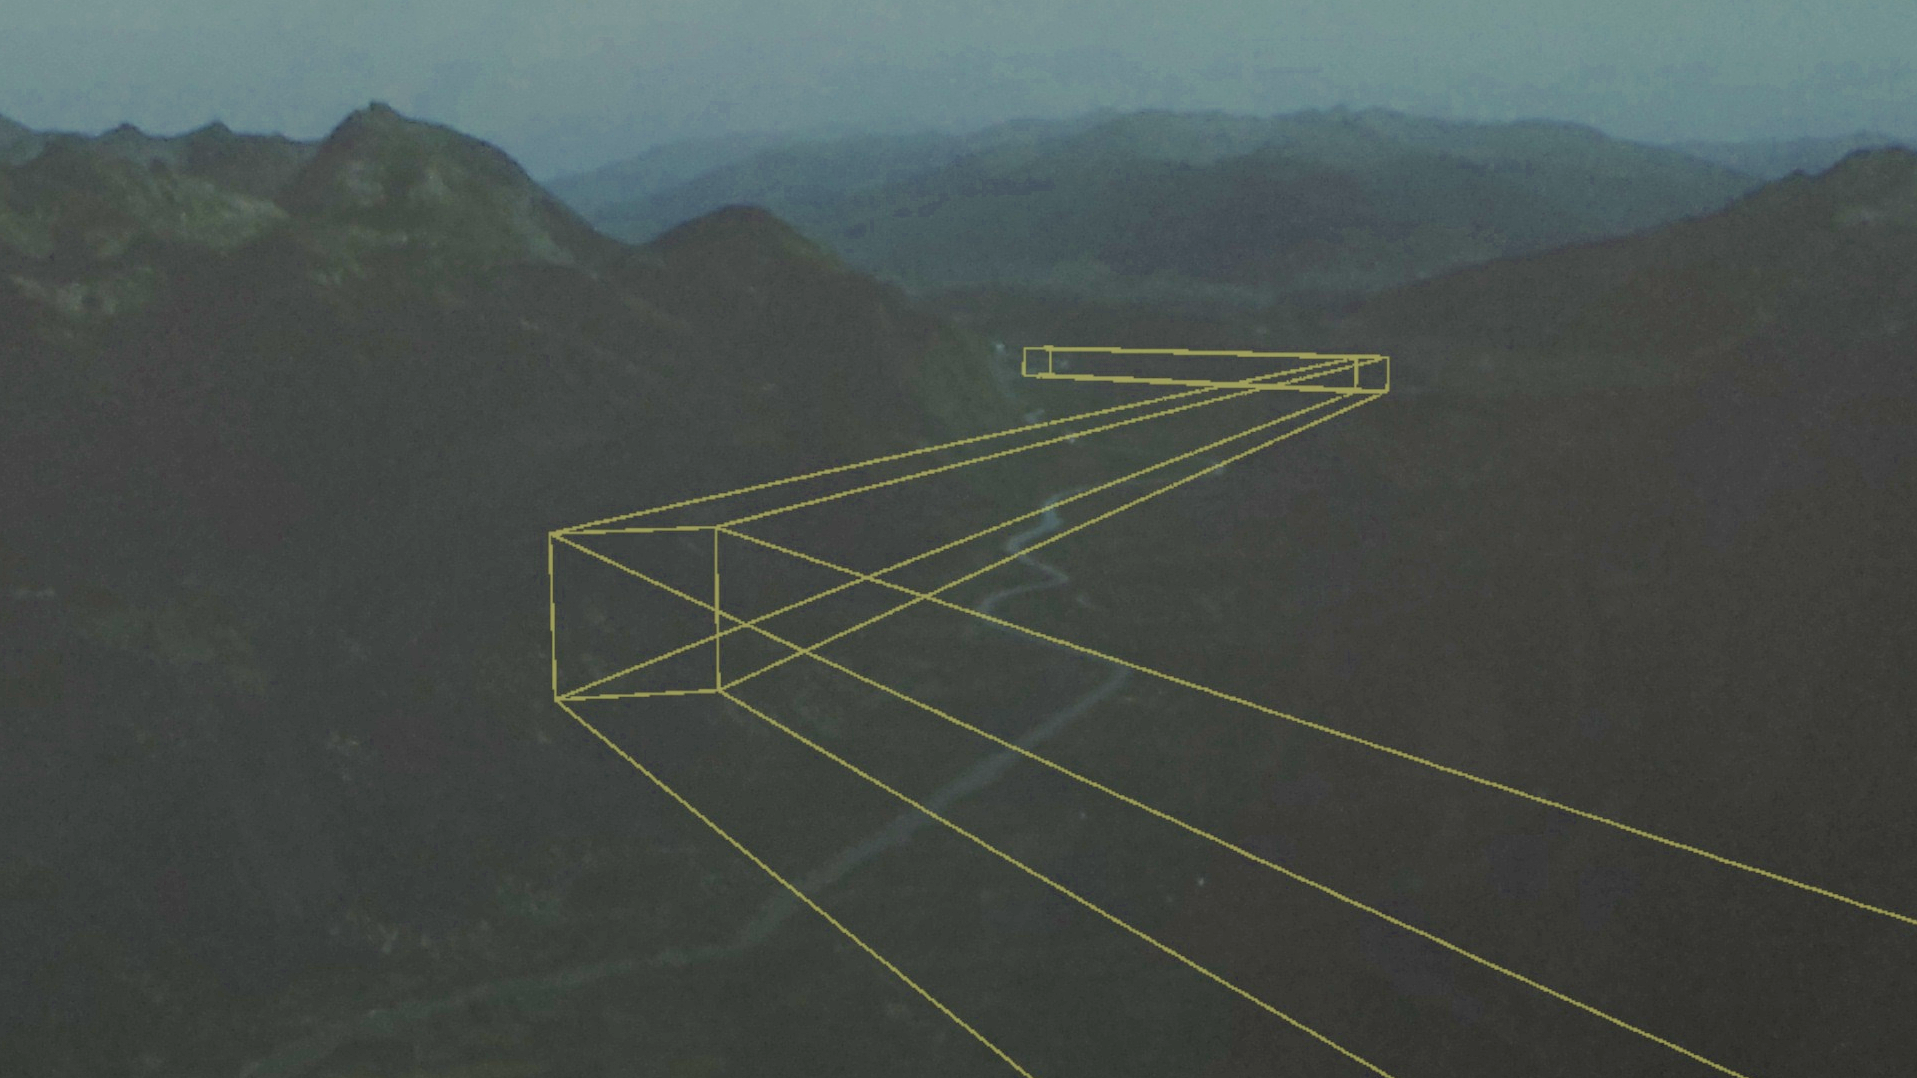
\includegraphics[width=0.6\textwidth]{tunnel-mesh-example.png}
  \caption{A visual example of a tunnel mesh. Each cross-sectional slice (vertical square) is placed at different geographical point with different orientations and is then connected to the others with straight segments.}\label{fig:tunnel_mesh_example.png}
\end{figure}

The details of \gls{holoassist}'s \gls{API} for \glspl{geofixedaug} are described in \autoref{appendix:external_meshes_api}, but in summary it is designed to offer a straightforward way of manipulating the vertex and index list for each \gls{gfelm}.

\subsection{Rendering geo-fixed external line meshes}\label{sec:renderling_elm}

The next step entails finding a way to convert such representation to something that can be understood by Unity, as computer graphics usually assumes a single, Euclidean space in which the various elements of the 3D scene are placed. As suggested in \cite{zintl_design_2020}, this result can be achieved by converting the vertices of all the \glspl{gfelm} to a common \gls{ENU} \acrlong{CRS} that is centered on the current geographical position of the aircraft, as computed by the flight simulator. Such \gls{ENU} \gls{CRS} is (rather unimaginatively) called the \enquote{\gls{planeENU}} in this document. This single \gls{CRS} is then mapped to the left-handed coordinate system used by Unity in such a way that it matches with the simulator's digital double described in \autoref{section:acquiring_digital_double}. This allows to treat all the \glspl{gfelm} as normal Unity meshes which are then rendered by the standard game engine rendering pipeline. A diagram summarizing the \glspl{CRS} involved in these conversions is available in \autoref{fig:crs_dataflow}. Implementing this algorithm requires:

\begin{figure}[p]
  \centering
  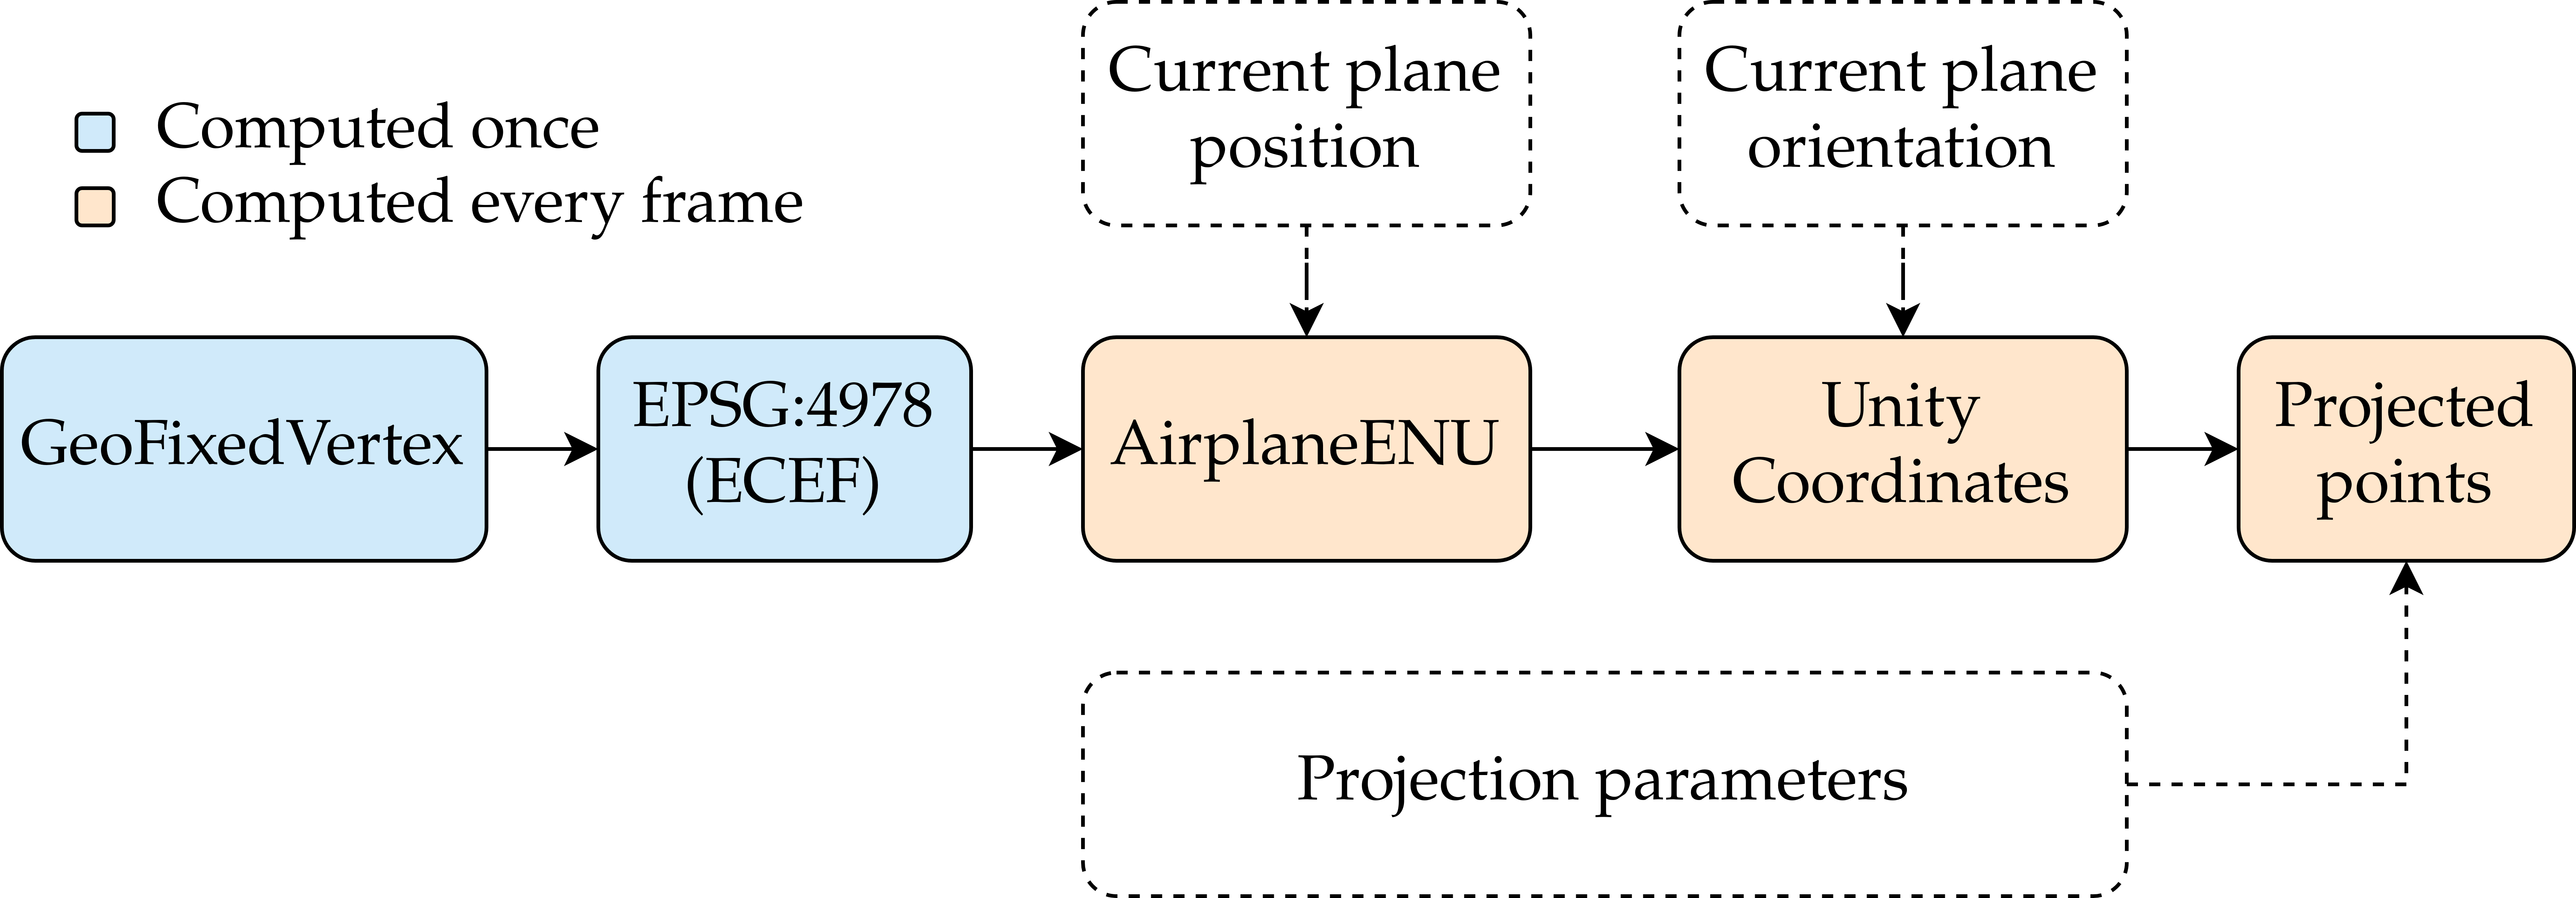
\includegraphics[width=0.8\textwidth]{crs_diagram.png}
  \caption{An overview of the transformations required to display a \texttt{GeoFixedVertex} at the correct position. Each of these conversions is explained in details in the main text. The last transformation is explained in \autoref{sec:projection_error}.}\label{fig:crs_dataflow}
\end{figure}

\begin{enumerate}
    \item Being able to obtain the airplane's current geographical position (and orientation) as computed by the flight simulator.
    \item Being able to convert a \texttt{GeoFixedVertex} to the \gls{planeENU}.
    \item Being able to convert a point from the \gls{planeENU} to the Unity \enquote{frozen} coordinate system in which the simulator digital double from \autoref{section:acquiring_digital_double} is placed.
\end{enumerate}

Acquiring the airplane's current geographical position and orientation from the flight simulator is straightforward, as most flight simulators have a way of broadcasting this information via \gls{UDP} packets. \gls{holoassist} is therefore capable of receiving this kind of information by listening on a \gls{UDP} port where it expects binary \gls{UDP} packets with the structure defined in \autoref{table:sim_status_update_udp_packet}. In this document, such packets are called \enquote{simulator status update} packets. Flight simulators can directly send simulator status update packets with that structure to \gls{holoassist} or an intermediate script can be written to translate the format used by the simulator to the one used by \gls{holoassist}.

\begin{table}[p]
  \centering
  \begin{tabular}{c c c c}
    \toprule
      Offset & Length & Type & Description \\
    \midrule
      0 & 1 & \-- & Fixed value (00000000) \\
      1 & 8 & double & Airplane current latitude in radians \\
      9 & 8 & double & Airplane current longitude in radians \\
      17 & 8 & double & Airplane current altitude in meters \\
      25 & 8 & double & Airplane current roll angle in radians \\
      33 & 8 & double & Airplane current pitch angle in radians \\
      41 & 8 & double & Airplane current yaw angle in radians \\
    \bottomrule
  \end{tabular}
  \caption[Structure of a simulator status update packet]{Describes the binary structure of a simulator status update \gls{UDP} packet. Field offset and length are in bytes. The field type \enquote{double} is a shorthand to indicate a IEEE 754 double-precision number encoded in little endian. The first byte of the packet is used to differentiate a simulator status update packet from other types of \gls{UDP} packets received on the same \gls{UDP} port.}\label{table:sim_status_update_udp_packet}
\end{table}

\begin{table}[p]
  \centering
  \begin{tabular}{c c}
    \toprule
      ENU axis & Unity axis\\
    \midrule
      Positive North & Positive Z\\
      Positive Up & Positive Y\\
      Positive East & Positive X\\
    \bottomrule
  \end{tabular}
  \caption{Mapping between Unity's coordinate system and the \gls{planeENU} when the airplane has zero yaw, pitch and roll.}\label{table:enu_to_unity_mapping}
\end{table}

Once the current geographical position of the aircraft is available to \gls{holoassist}, it becomes possible to compute the position of each \texttt{GeoFixedVertex} in the \gls{planeENU}. This happens in two phases. The first phase entails converting each \texttt{GeoFixedVertex} to the \gls{ECEF} \gls{CRS}: this conversion is perfomed once when the vertex is created via the \gls{API}. Denoting with the \gls{epsg4979} point $\mathbf{o}$ the topocentric origin of the \texttt{GeoFixedVertex}, with $\mathbf{t} \in \mathbb{R}^3$ its local translation and with $R_l \in \mathbb{R}^{3\times 3}$ the rotation matrix describing its local rotation, the \gls{ECEF} coordinates are computed as follows:

\begin{equation}
    \label{eq:externallinemeshvertextoecef}
    \mathbf{v}_{\text{ECEF}} = \convertENUtoECEF{R_l \mathbf{t}}{\mathbf{o}}
\end{equation}

Where $\convertENUtoECEF{\cdot}{\cdot}$ is the function defined in \autoref{eq:convertENUtoECEF}. The second phase happens once per rendered frame and entails converting each $\mathbf{v}_{\text{ECEF}}$ to the \gls{planeENU}:

\begin{equation}
    \mathbf{v_{\text{AirplaneENU}}} = \convertECEFtoENU{\mathbf{v}_{\text{ECEF}}}{\mathbf{q}}
\end{equation}

Where $\mathbf{q}$ is the current airplane position in \gls{epsg4979} as received from the simulator and $\convertECEFtoENU{\cdot}{\cdot}$ is defined in \autoref{eq:convertECEFtoENU}. Technically, this conversion would only need to be performed once per simulator status update. However, since the simulator in which \gls{holoassist} has been tested broadcasts updates frequently enough to be comparable with the Hololens' framerate, it was decided to recompute it once per frame. Moreover, this keeps the workload consistent across frames, improving hologram's stability\cite{microsoft_corporation_hologram_nodate}.

Now that all the vertices of the \glspl{gfelm} are expressed in a single Euclidean space (the \gls{planeENU}), the last step is to map it to the same Unity's frozen coordinate space in which the simulator digital double is positioned as described in \autoref{section:acquiring_digital_double}. In order to simplify this step, some additional requirements on the coordinates that are chosen for the space pins described in \autoref{section:aligning_virtual_with_real_world} are necessary. As of now, the concrete values of the coordinates of the space pins have been irrelevant, as long as the relative offset between them is consistent with the real-world offset between the QR codes. However, in order to easily map the \gls{planeENU} to Unity's coordinate system, those coordinates need to be picked in such a way that the simulator digital double's longitudinal axis is aligned with Unity's Z axis and that the digital double's vertical axis is aligned with Unity's Y axis.

When this additional requirement is added we can observe that, if the plane geographical orientation computed by the simulator is zero on all three axes (yaw, pitch, roll), then Unity's Z axis (and therefore the digital double's longitudinal axis) is aligned with the \gls{planeENU} north axis, as an airplane with a yaw of zero degrees is pointing north. Moreover, due to the roll and pitch of zero degrees, the \gls{planeENU} up axis is aligned with Unity's Y axis (and therefore with the digital double's vertical axis). This means that, if the plane has no geographical rotation and all the requirements are uphold, the \gls{planeENU} space can be mapped to Unity's coordinates with the mapping described in \autoref{table:enu_to_unity_mapping} and the result will visually match in the real world with what can be seen from the simulator cockpit's windows. An example of this axes alignment is shown in \autoref{fig:axis_alignment}.

\begin{figure}
  \centering
  \subfloat[\Gls{planeENU}'s East, North, Up axes]{\includegraphics[height=0.35\textwidth]{unity-axes-enu.png}}
  \hfill
  \subfloat[Unity's X, Y, Z axes]{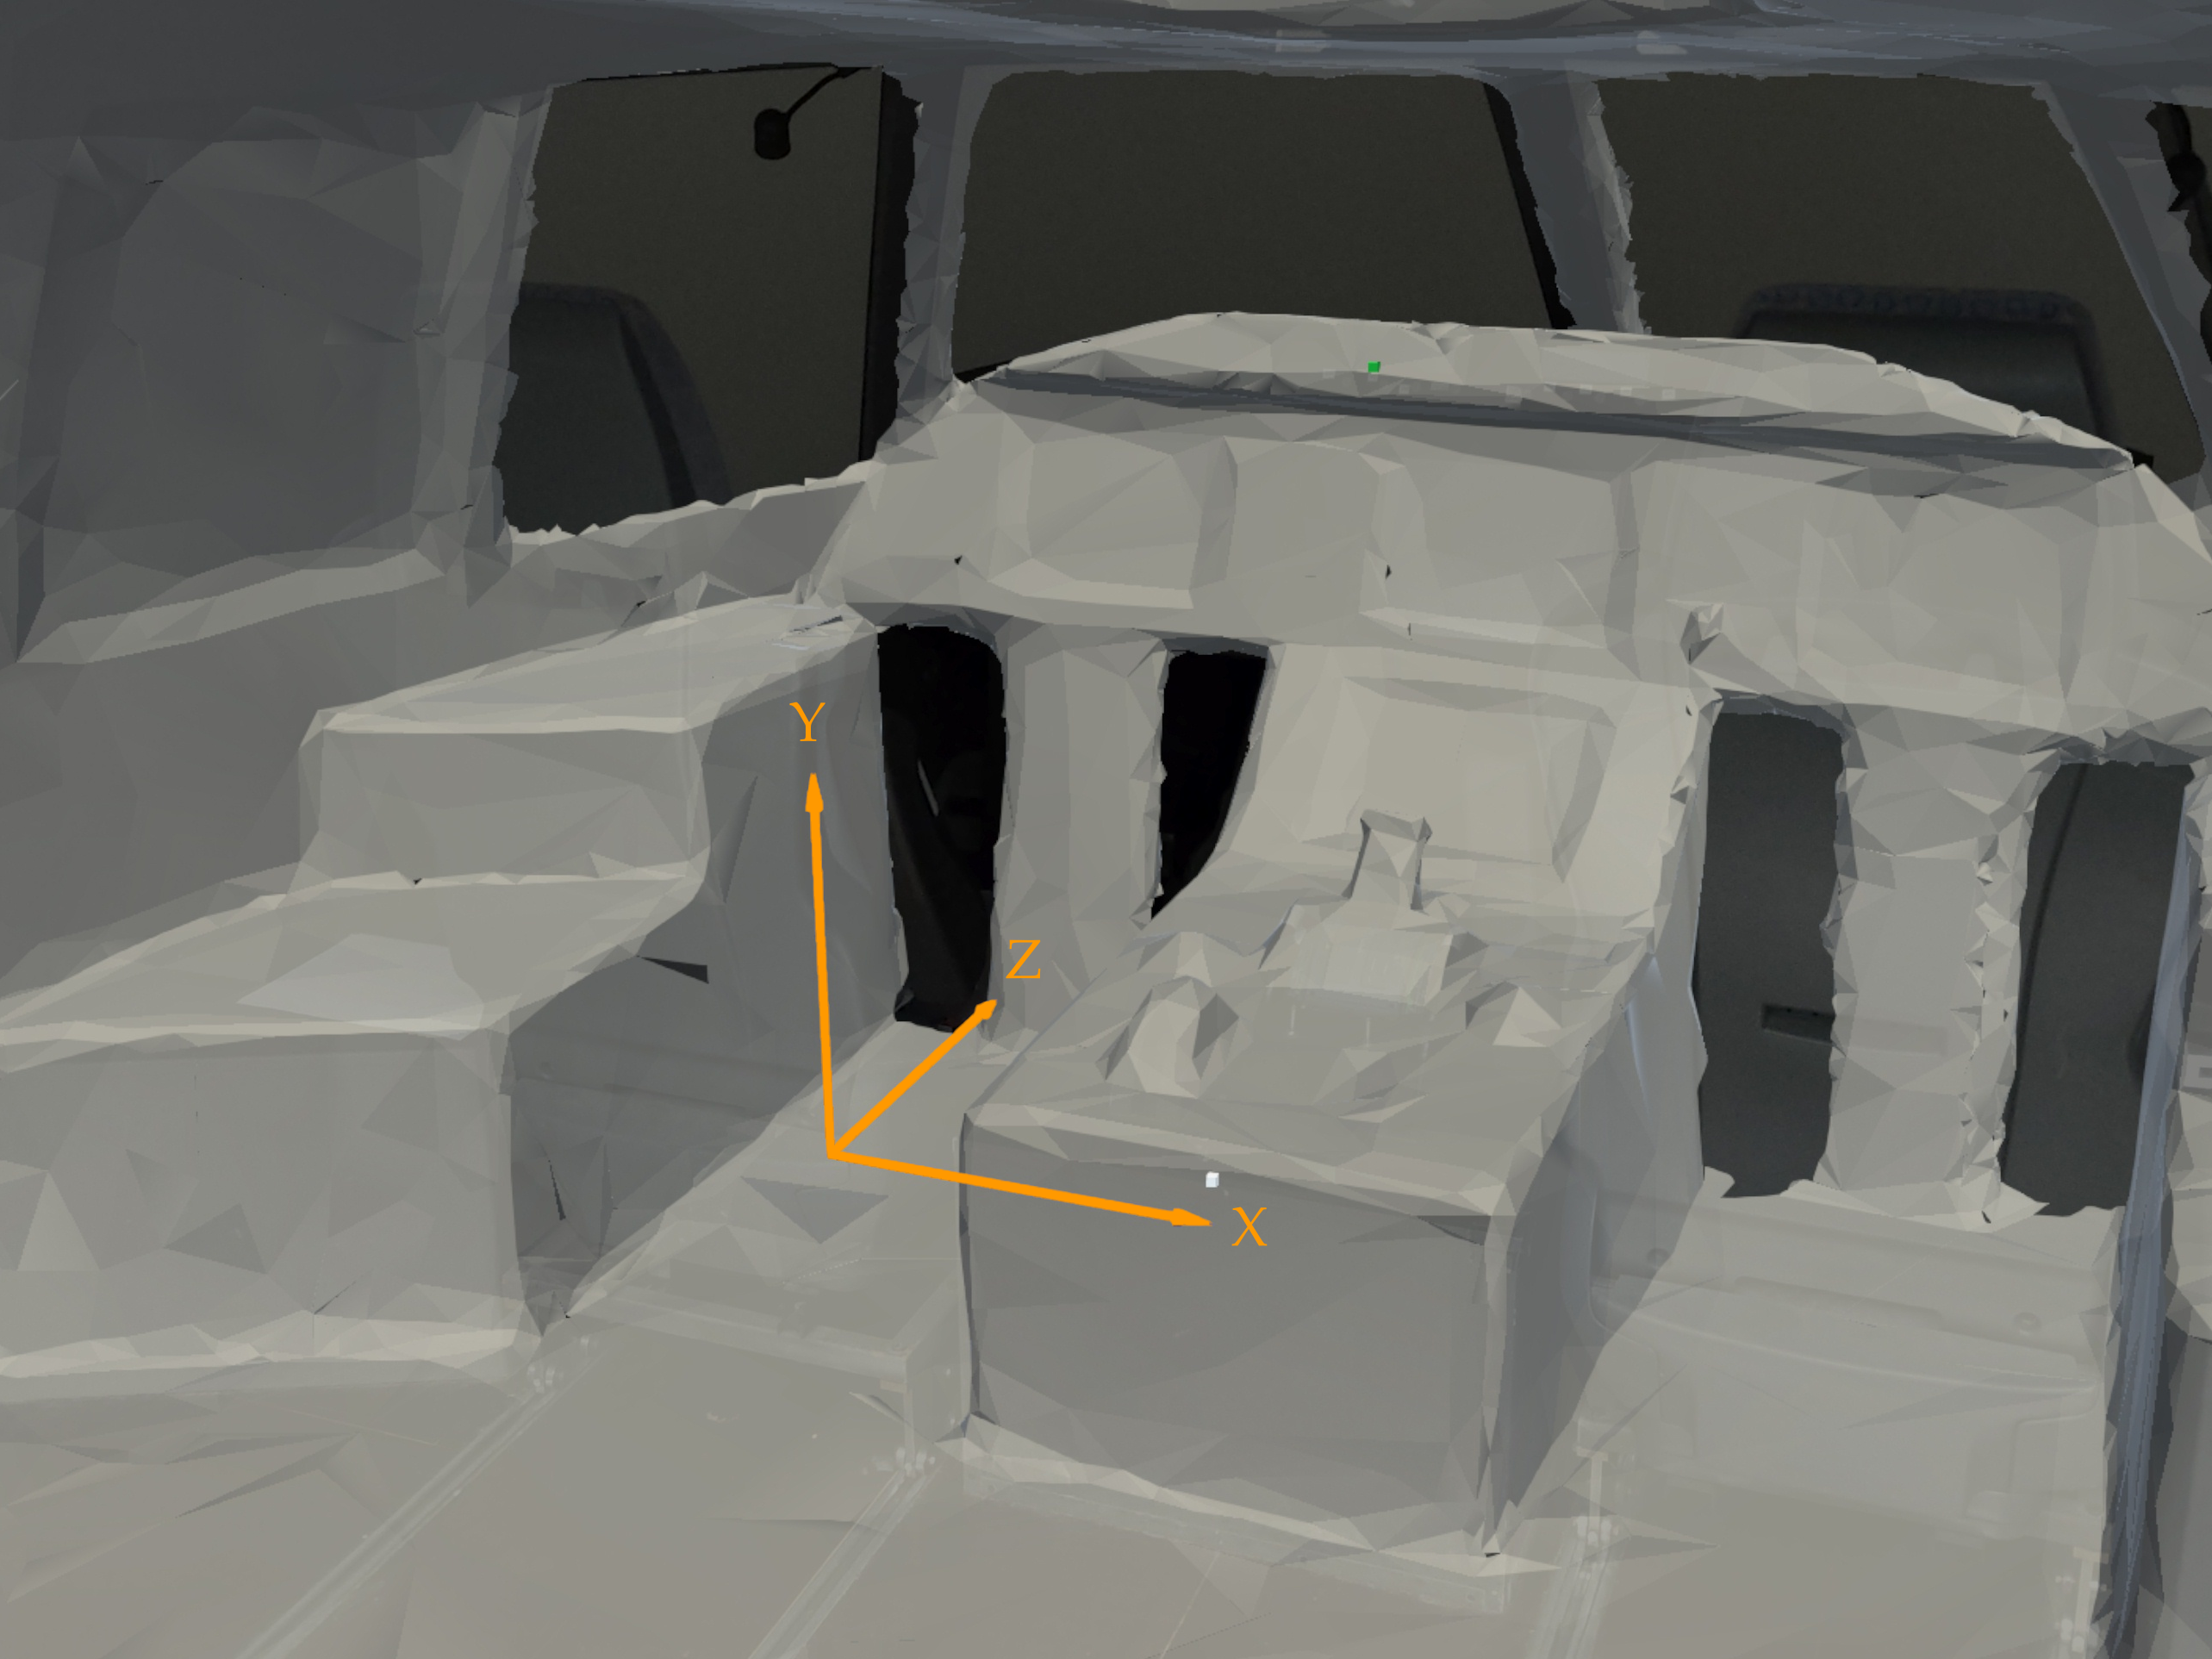
\includegraphics[height=0.35\textwidth]{unity-axes-unity.png}}
  \caption{An image taken from the Hololens while running \gls{holoassist} that shows the alignment between the real simulator, the Unity coordinate system and the \gls{planeENU}. When the airplane has zero yaw, pitch and roll, the simulator's longitudinal axis is aligned with Unity's Z axis and the \gls{planeENU} N axis. The same happens for the simulator's vertical axis, Unity's X axis and the \gls{planeENU} U axis.}\label{fig:axis_alignment}
\end{figure}


However, this simple mapping is not sufficient. The aircraft position computed by the flight simulator is usually the geographical position of the aircraft's center of mass. In order to obtain correctly placed \glspl{geofixedaug} we need to take into account the offset between this point and the simulator digital double. The offset between the airplane center of mass and the simulator cockpit is usually available in the simulator's documentation. \gls{holoassist} expects that the position of the aircraft's center of mass in the Unity frozen world (see \autoref{section:aligning_virtual_with_real_world}) is supplied as a simulator-specific value in the same JSON file in which the virtual locations for the various space pins are recorded. For the simulator in which \gls{holoassist} was tested, this looks like \autoref{lst:plane_center_of_mass_virtual_positions_json}.

\begin{figure}
  \centering
  \begin{tabular}{c}
  \begin{lstlisting}[language=json]
    {
        "planeCenter": [0, 2.1336, -10.0584],
        "spacePins": {
            // all the space-pins locations
        },
        // other simulator-related information not relevant here
    }
  \end{lstlisting}
  \end{tabular}
  \caption{An extract of the JSON file that describes the virtual positions of the plane center of mass.}\label{lst:plane_center_of_mass_virtual_positions_json}
\end{figure}

The last piece of the puzzle regards the airplane geographical orientation, which is supplied by the simulator as part of the simulator status update. Since \gls{holoassist} is designed for fixed-platform simulators, when the geographical orientation of the aircraft changes, the simulator cockpit doesn't actually move in the real world: the only thing that changes is the imagery that is visible through the cockpit windows. Therefore, the virtual position of the simulator digital double cannot be changed, as it needs to remain aligned with the real cockpit: thus, when the airplane changes geographical orientation, instead of rotating the digital double, the inverse of such rotation is applied when matching the \gls{planeENU} with the Unity's coordinate system.

Combining all these considerations allows for a mapping from the \gls{planeENU} to the Unity's coordinate system that ensures visually correct \glspl{geofixedaug}. More formally, let $\mathbf{b} \in \mathbb{R}^3$ be the position of the airplane center of mass in Unity's coordinate system, let $R_{g} \in \mathbb{R}^{3\times3}$ be the rotation matrix\footnote{Although the descriptions in this document represent rotations with $3\times3$ matrices, internally \gls{holoassist} uses quaternions\cite{noauthor_quaternions_2022}, as they are the standard implementation for handling rotations in game engines. However, quaternion details tend to be less known, and therefore the more common matrix representation has been chosen.} describing the current airplane rotation as obtained from the simulator and let $\mathbf{v}_{\text{AirplaneENU}} \in \mathbb{R}^3$ be the position of a \texttt{GeoFixedVertex} converted to the \gls{planeENU} for the current frame. Then that point's position in the Unity space is computed as follows:

\begin{equation}
    \mathbf{v}_{\text{Unity}} = \mathbf{b} + R_g^{-1} M\mathbf{v}_{\text{AirplaneENU}}
\end{equation}

With $M$ encoding the mapping described in \autoref{table:enu_to_unity_mapping}:

\begin{equation}
    M = \begin{pmatrix} 1 & 0 & 0 \\ 0 & 0 & 1 \\ 0 & 1 & 0\end{pmatrix}
\end{equation}

The airplane's geographical orientation coming from the simulator status updates is assumed to be in a right-handed coordinate system with the \enquote{up} axis pointing downwards: when computing $R_g$, appropriate care should be taken to convert the rotation to the left-handed coordinate system that Unity uses and to also account for the different orientation of the \enquote{up} axis.

At this point, the process to convert from \gls{gfelm} vertices to positions that are understood by Unity is complete: these converted positions are then handed to the game engine as normal 3D meshes (instances of the \texttt{CoreModule.Mesh} class), which are rendered by the standard rendering pipeline, yielding a visual result which shows the virtual augmentation at the desired geographical position when looking outside the simulator windows in the real world.

\subsection{Accounting for projection error}\label{sec:projection_error}

Although the steps described in the previous sections are correct for a real aircraft, in a fixed-platform flight simulator they will yield a result that is visually wrong, as shown in \autoref{fig:no_projection_is_wrong.png}. This is due to how fixed-platform simulators usually work. As shown in \autoref{fig:sim_structure.png}, a fixed-platform simulator is usually composed of a cockpit, which resembles the real plane and where the pilot sits, and a (usually cylindrical) screen placed in front of it. The simulator then uses some projectors to show on this screen what the pilot would see from the cockpit's window at the current geographical position of the plane. In order to do this, the simulator engine has to project geographical features that in the real world would be placed kilometers away from the airplane to the cylindrical screen a few meters in front of the cockpit: this kind of projection can be computed correctly only for a single point, known as the \gls{PEP}, which is usually placed inside the cockpit, near the head of the pilot. A viewer placed in any other position than the \gls{PEP} will see some projection error in what is shown on the outside screen.

\begin{figure}
  \centering
  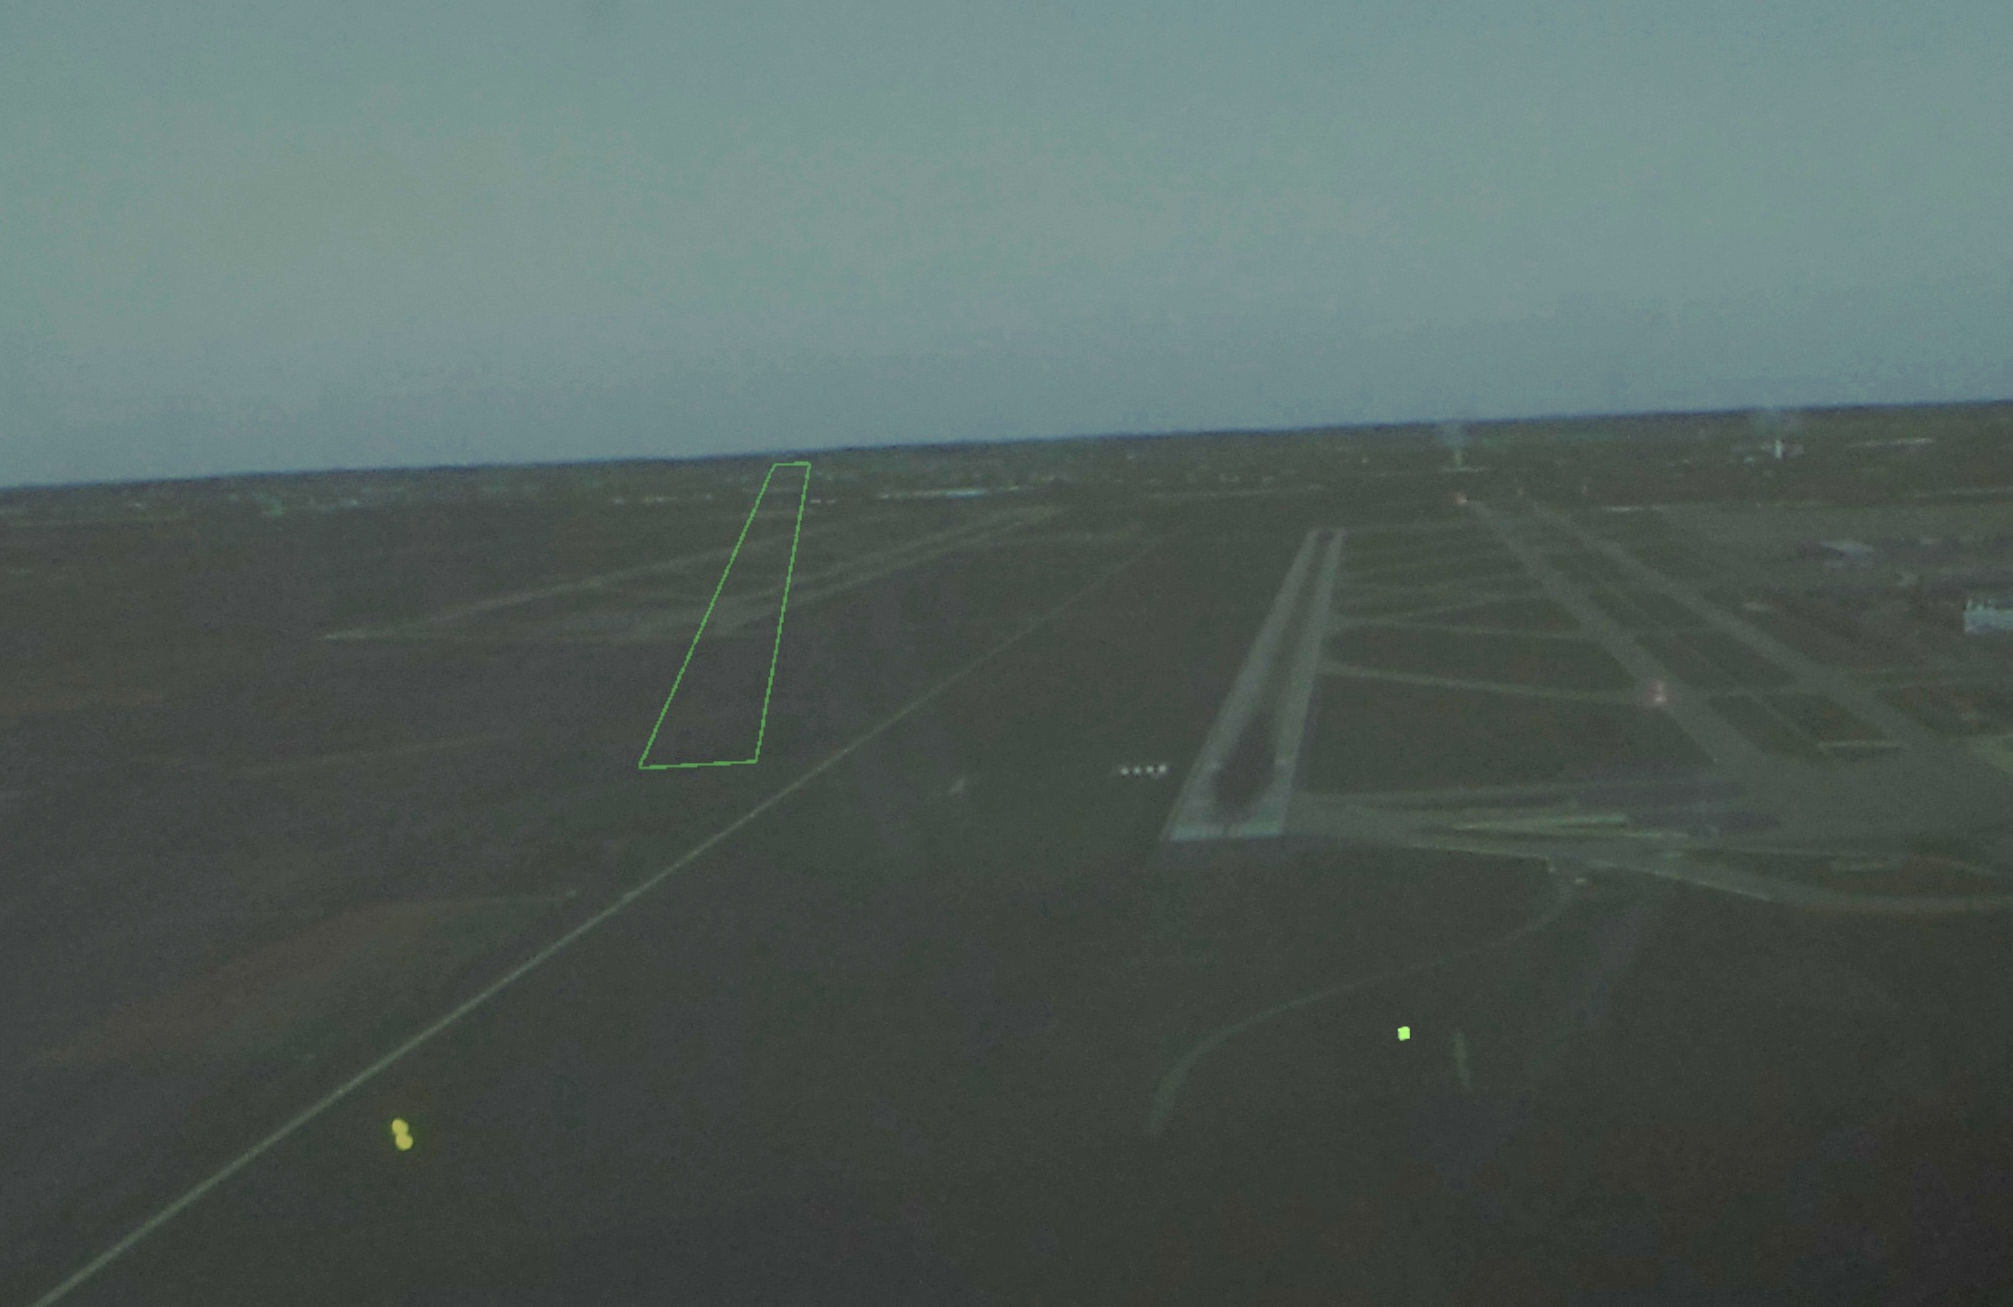
\includegraphics[width=0.8\textwidth]{munich-runway-projection-off.png}
  \caption{An image taken from the Hololens while running \gls{holoassist} that shows a \gls{geofixedaug} for the runway of an airport. Although the computations are correct, the result does not visually match the image produced by the simulator.}\label{fig:no_projection_is_wrong.png}
\end{figure}

\begin{figure}
  \centering
  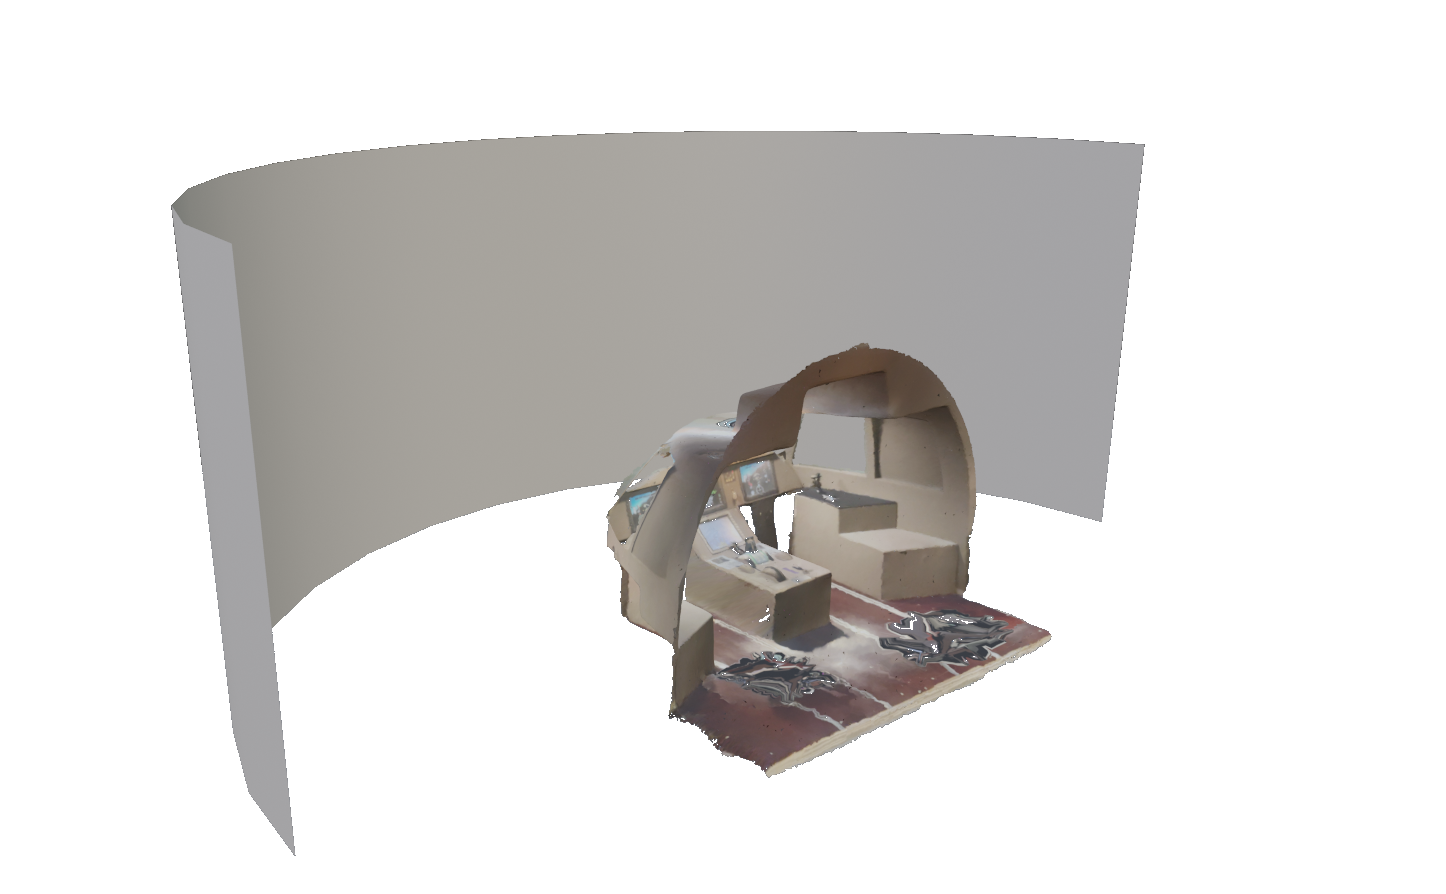
\includegraphics[width=0.8\textwidth]{simulator-structure.png}
  \caption{An overview of the structure of a fixed-platform flight simulator. In the center there is a replica of the cockpit of the airplane being simulated, and in front of it there is a (often cylindrical) screen on which the imagery generated by the simulator is projected.}\label{fig:sim_structure.png}
\end{figure}

This is usually not a huge issue, as the projected imagery still looks real and precise, but becomes relevant when we want to add some augmentations on top of real world features. The computations described in the previous sections do not account for this projection error, and therefore, despite being correct, they appear visually wrong if the Hololens is positioned in any point other than the \gls{PEP}, as shown in \autoref{fig:no_projection_correct_around_pep.png}. In order to obtain visually correct results in every place inside the simulator we need to apply the same projection used by the flight simulator to the $\mathbf{v}_{\text{Unity}}$ coordinates computed in \autoref{sec:renderling_elm}.

\begin{figure}
  \centering
  \subfloat[Left of the \gls{PEP}]{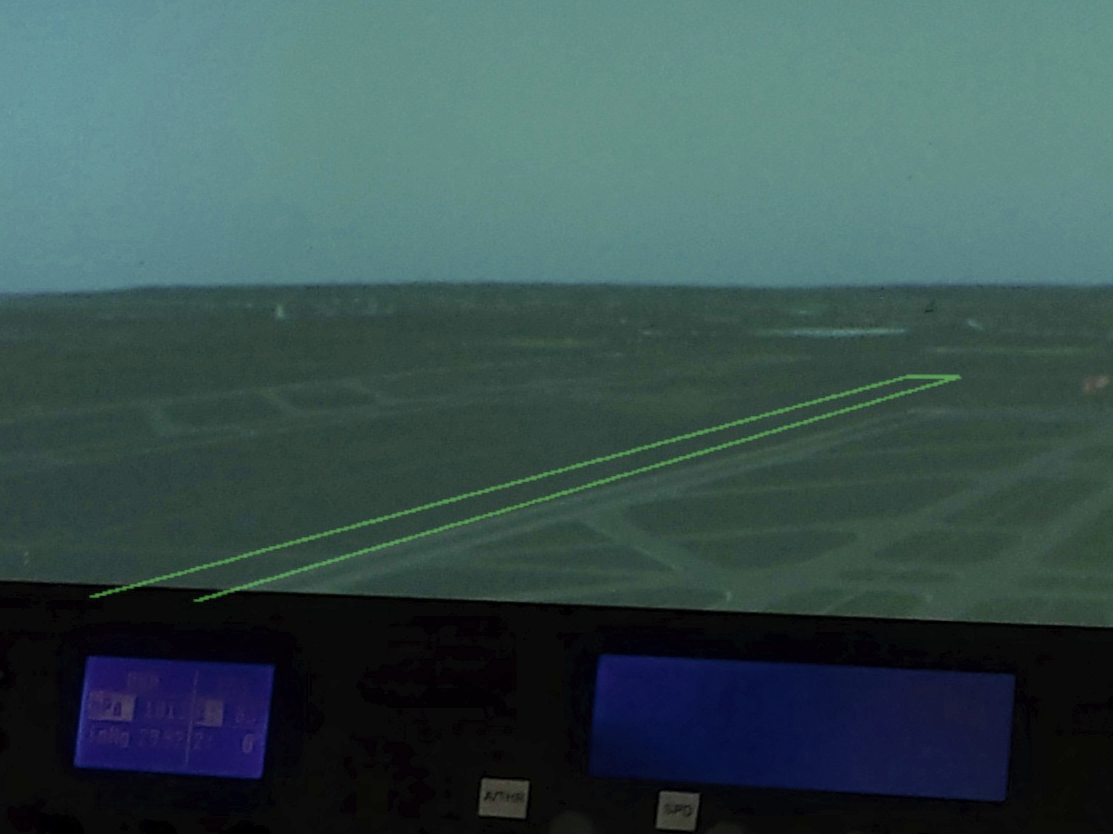
\includegraphics[height=0.35\textwidth]{head-left-pep.png}\label{fig:no_proj_around_pep_left}}
  \hfill
  \subfloat[Right of the \gls{PEP}]{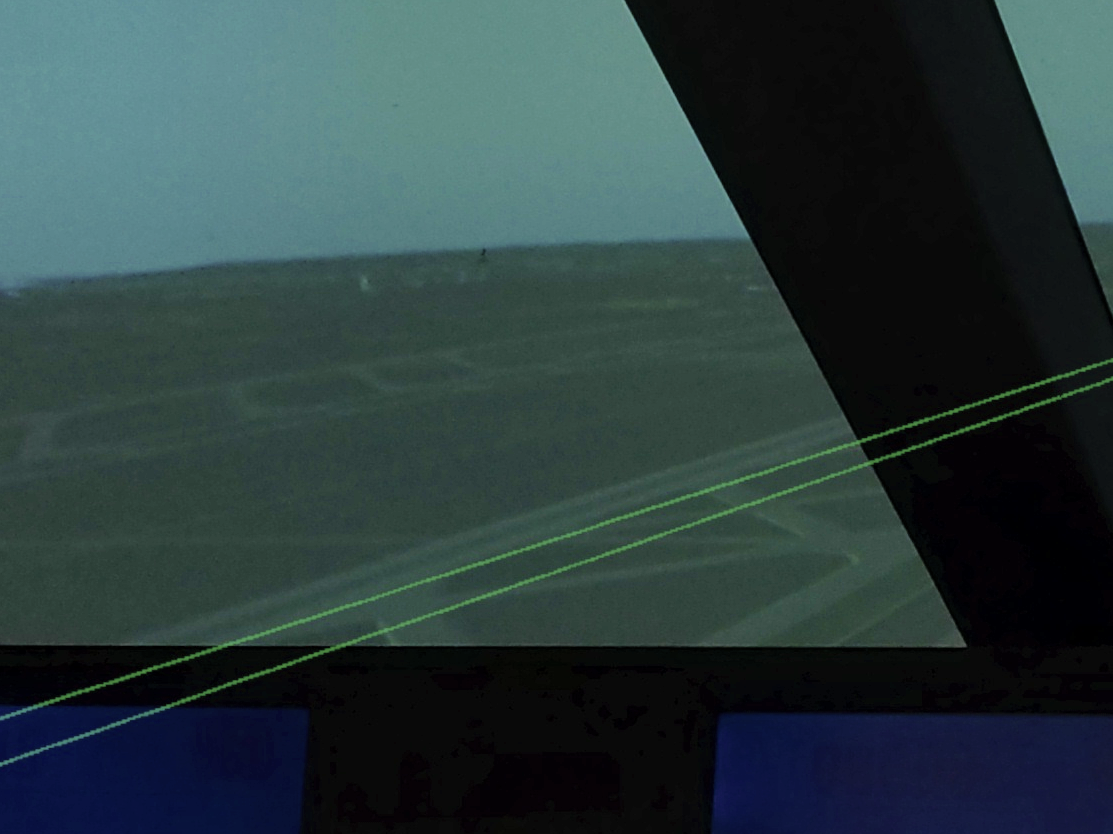
\includegraphics[height=0.35\textwidth]{head-right-pep.png}\label{fig:no_proj_around_pep_right}}
  \caption{Images taken from the Hololens of a \gls{geofixedaug} being shown without the correction for the projection error. Each image shows the visual output at a different position with respect to the \gls{PEP}.}
\label{fig:no_projection_correct_around_pep.png}
\end{figure}

In order to do this, a few additional simulator-specific parameters are needed. They are:

\begin{enumerate}
    \item The shape of the projection screen. In the simulator in which \gls{holoassist} is tested the projector screen is assumed to be a cylinder with its axis parallel to the airplane's vertical axis.
    \item The position of the center of the cylinder in the virtual world. Let this point in the virtual Unity frozen space be called $\mathbf{c} \in \mathbb{R}^3$.
    \item The radius of the cylinder, which will be called $r \in \mathbb{R}$.
    \item The position of the \gls{PEP} in the virtual world. Let this point in the virtual Unity frozen space be called $\mathbf{e} \in \mathbb{R}^3$.
\end{enumerate}

These values can usually be derived from the simulator documentation. However, as the simulator in which \gls{holoassist} is tested is a non-commercial research simulator, these value had to be obtained in another way, described in \autoref{sec:obtaining_rfs_measures}. Once known, these values are stored in the same simulator-specific JSON file in which the virtual position of the space pin are stored. An example is shown in \autoref{lst:plane_projection_params_json}.

\begin{figure}
  \centering
  \begin{tabular}{c}
  \begin{lstlisting}[language=json]
    {
        "projection": {
            "type": "CYLINDER",
            "cylinderCenter": [ 0.960499, -1.262993, 0.286 ],
            "cylinderRadius": 4.012081,
            "eyePoint": [ 0.989999, -0.552001, 0.686999]
        },
        "spacePins": {
            // all the space-pins locations
        },
        // other simulator-related information not relevant here
    }
  \end{lstlisting}
  \end{tabular}
  \caption{An extract of the JSON file that describes the parameters needed to account for the projection error.}\label{lst:plane_projection_params_json}
\end{figure}

Given the above-mentioned parameters $\mathbf{c}$, $r$ and $\mathbf{e}$ and a point $\mathbf{v}_{\text{Unity}}$ as computed above, the projection $\mathbf{v}_{\text{proj}}$ of such point to the cylinder surface can be computed similarly to how it is done in \cite{walko_integration_2020}. In the cylindrical screen case, the geometrical setup of the problem is shown in \autoref{projection_setup.png}, in which the unknown is $\mathbf{v}_{\text{proj}}$. The direction of the line connecting $\mathbf{v}_{\text{Unity}}$ and the \gls{PEP} can be computed as follows:

\begin{figure}
  \centering
  \subfloat[Top view]{
\includegraphics[height=0.35\textwidth]{projection-setup-2.png}}
  \hspace{1cm}
  \subfloat[Side view]{
\includegraphics[height=0.35\textwidth]{projection-setup-1.png}}
  \caption{The top and side views of the geometrical setup for the projection of a point in the \gls{planeENU} space to the cylindrical screen.}\label{projection_setup.png}
\end{figure}

\begin{equation}
    \mathbf{n} = \frac{\mathbf{v}_{\text{Unity}} - \mathbf{e}}{\lVert\mathbf{v}_{\text{Unity}} - \mathbf{e}\rVert}
\end{equation}

Therefore, the line connecting them is:

\begin{equation}
    D(t) = \mathbf{e} + t \mathbf{n}
\end{equation}

Similarly, the axis of the cylinder can be written as:

\begin{equation}
    C(t) = \mathbf{c} + t \hat{\mathbf{y}}
\end{equation}

Where $\hat{\mathbf{y}}$ is the unit-length vector denoting the Unity Y axis, which is parallel to the simulator digital double vertical axis and to the cylinder axis. In order to find $\mathbf{v}_{\text{proj}}$ we need to find the value $d \in \mathbb{R}$ for which the line $D(d)$ intersects the cylinder, that is, the value of $d$ for which the point $D(d)$ is at distance $r$ from the line $C(t)$:

\begin{equation}
    \label{eq:projection_condition}
    \text{distance}\left(C(t), D(d)\right) = r
\end{equation}

Given a line $\mathbf{a} + x \mathbf{b}$, its distance from a generic point $\mathbf{p}$ is given by\cite{noauthor_distance_2021}:

\begin{equation}
    \text{distance}\left(\mathbf{a} + x\mathbf{b}, \mathbf{p}\right) = \lVert \left(\mathbf{p} - \mathbf{a}\right) - \left(\left(\mathbf{p} - \mathbf{a}\right) \cdot \mathbf{b} \right) \cdot \mathbf{b} \rVert
\end{equation}

\autoref{eq:projection_condition} can be rewritten as follows:
\begin{IEEEeqnarray}{rCl}
    \text{distance}\left(C(t), D(d)\right) & = & r \\
    \text{distance}\left(\mathbf{c} + t\hat{\mathbf{y}}, \mathbf{e} + d \mathbf{n}\right) & = & r \\
    \lVert \left(\mathbf{e} + d\mathbf{n} - \mathbf{c}\right) - \left(\left(\mathbf{e} + d\mathbf{n} - \mathbf{c}\right) \cdot \hat{\mathbf{y}} \right) \cdot \hat{\mathbf{y}}\rVert & = & r\\
    & \text{\ldots} & \\
    \left\lVert \begin{pmatrix}e_1 + d n_1 - c_1 \\ 0 \\ e_3 + d n_3 - c_3\end{pmatrix} \right\rVert & = & r \\
    \left(e_1 + dn_1 - c_1\right)^2 + \left(e_3 + dn_3 - c_3\right)^2 & = & r^2
\end{IEEEeqnarray}

Where the $x_i$ syntax denotes the $i$-th element of vector $\mathbf{x}$. The last step of the derivation is a second degree equation in $d$ that can be solved with standard techniques, yielding two solutions $d_1$ and $d_2$, one for the \enquote{entry point} of the line in the cylinder and one for the \enquote{exit point}. Assuming the direction from $\mathbf{v}_{\text{Unity}}$ to $\mathbf{e}$, the desired point is always the entry point, which given this setup is the closest to $\mathbf{v}_{\text{Unity}}$. Therefore, the desired $d$ is:

\begin{equation}
    d = \min\left(\lVert D(d_1) - \mathbf{v}_{\text{Unity}} \rVert, \lVert D(d_2) - \mathbf{v}_{\text{Unity}} \rVert\right)
\end{equation}

Thus, the actual final output of the conversion of a \texttt{GeoFixedVertex} to Unity coordinates is:

\begin{equation}
    \mathbf{v}_{\text{proj}} = D(d)
\end{equation}

After applying this step, \gls{geofixedaug} appear visually correct from all points of the simulator, as shown in \autoref{fig:munich_runway_highlighted_shown_from_different_positions.png}.

\begin{figure}
  \centering
  \subfloat[Left of the \gls{PEP}]{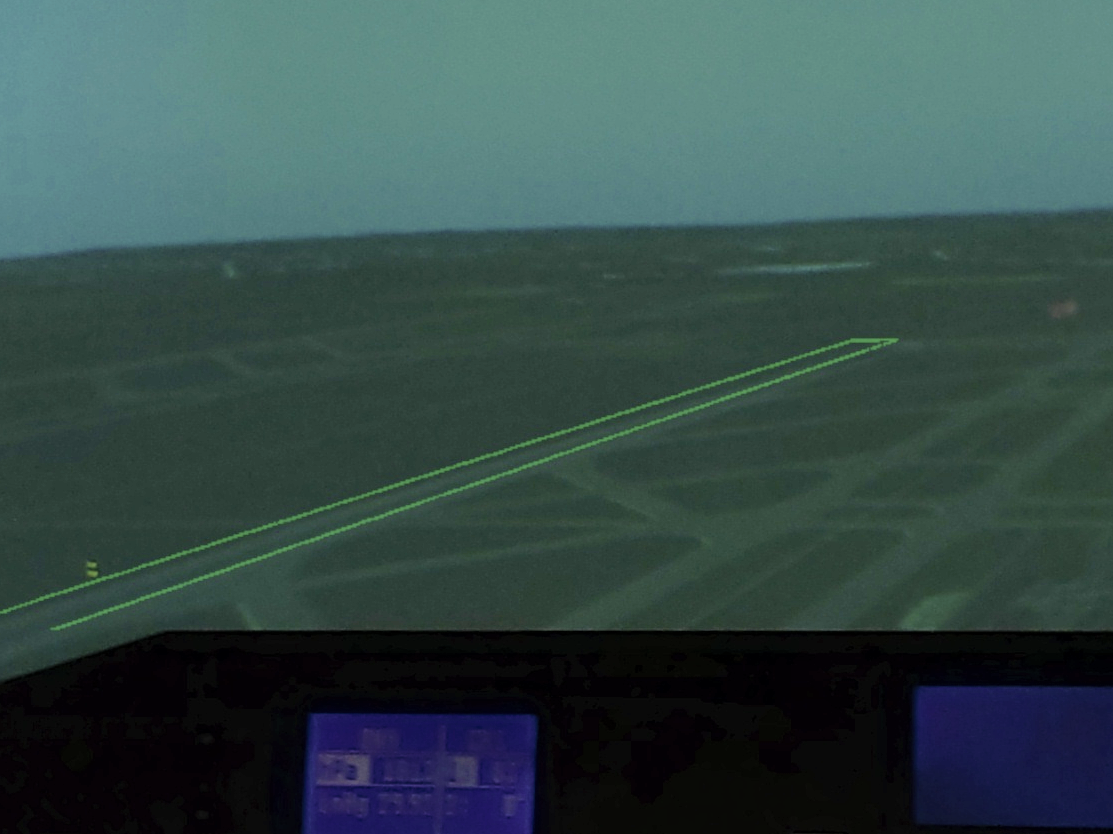
\includegraphics[height=0.35\textwidth]{head-left-pep-proj-on.png}}
  \hfill
  \subfloat[Right of the \gls{PEP}]{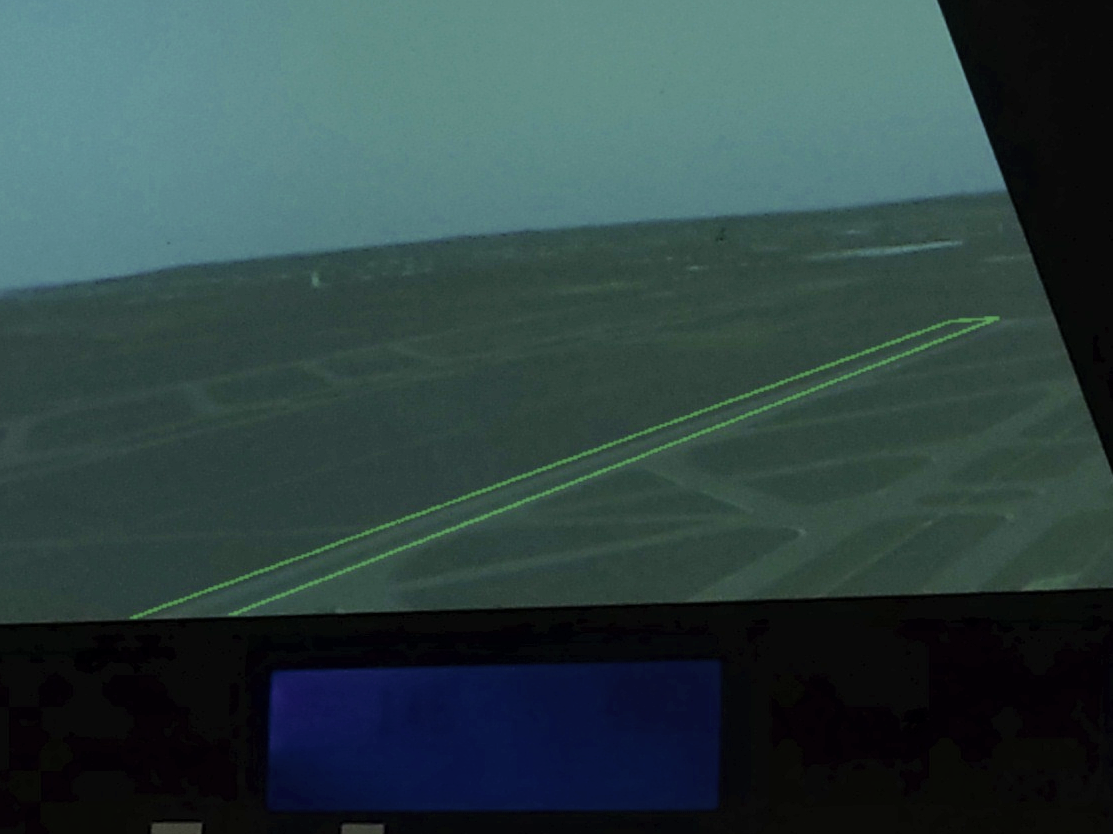
\includegraphics[height=0.35\textwidth]{head-right-pep-proj-on.png}}
  \caption{Images taken from the Hololens after applying the correction for the projection error. The \gls{geofixedaug} now appears visually correct from every head position.}
\label{fig:munich_runway_highlighted_shown_from_different_positions.png}
\end{figure}

However, applying the projection in this way introduces a limitation to the kind of meshes that the current version of \gls{holoassist} can show. Flattening all vertices to the same cylindrical surface as the projection does completely removes all the depth information that would normally be associated with the mesh's triangles and that would be used to distinguish which triangle should be drawn in front of the others during the normal rendering pipeline (in a step called depth test\cite{khronos_group_depth_nodate}). Although this problem should be solvable by manually reimplemening a mechanism analogous to the depth test applied to the cylinder surface, it was decided to not deal with this in the current version of \gls{holoassist}. It was instead decided to (more simply) limit the kind of mesh that could be shown: rather than allowing meshes with triangular topology, only meshes with linear topology (i.e.\ composed by lines) are permitted. This is the reason for which \glspl{gfelm} have \texttt{Line} in their name. Although this limits the kind of \gls{AR} augmentations that can be shown, it was deemed an acceptable trade-off because:

\begin{enumerate}
    \item The currently planned \glspl{geofixedaug} would have been line-based anyway;
    \item It was preferred to obtain something working earlier that could then be expanded in the future rather than delaying deployment until all features could be implemented\cite{gabriel_rise_1991}.
\end{enumerate}

\subsection{Automatic interpolation}\label{sec:automatic_interpolation}

Although the solution to the projection error shown in \autoref{sec:projection_error} works, it sometimes leads to an unexpected behavior. Take for example a \gls{geofixedaug} highlighting a landing strip of an airport, as shown in \autoref{fig:munich_runway_highlighted.png}. If the airplane flies directly over the landing strip at a low altitude, the unexpected outcome shown in \autoref{fig:munigh_runway_highligted_projection_not_interpolated.png} happens. This happens because the \gls{geofixedaug} only specifies four vertices for its \gls{gfelm}, one for each corner of the landing strip: these four vertices are then projected to the cylinder (correctly, as shown by the orange circle in \autoref{fig:munigh_runway_highligted_projection_not_interpolated.png}), but then are connected by straight lines, which therefore \enquote{cut through} the projection cylinder instead of wrapping around it as expected.

\begin{figure}
  \centering
  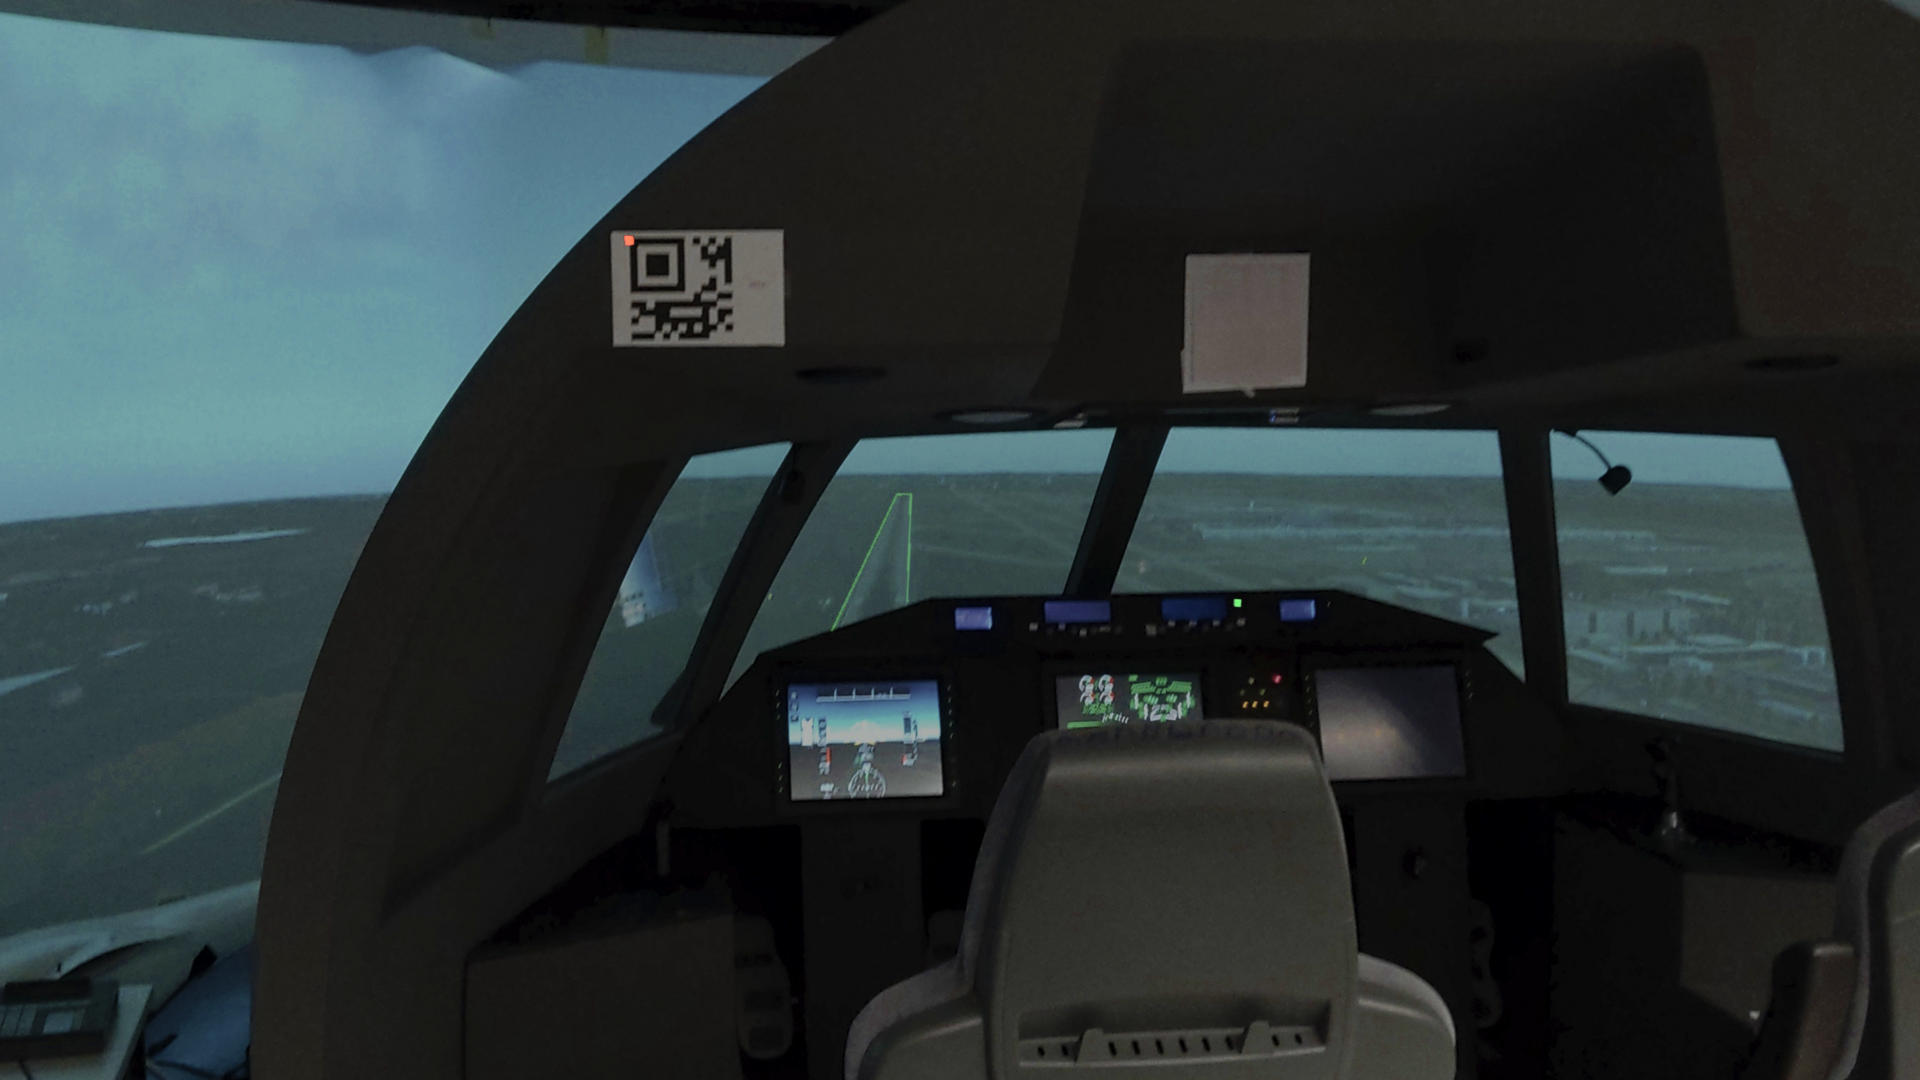
\includegraphics[width=0.8\textwidth]{munich-runway-no-interpolation-1.png}
  \caption{An image taken from the Hololens that shows a \gls{geofixedaug} highlighting the runway of an airport.}\label{fig:munich_runway_highlighted.png}
\end{figure}

\begin{figure}
  \centering
  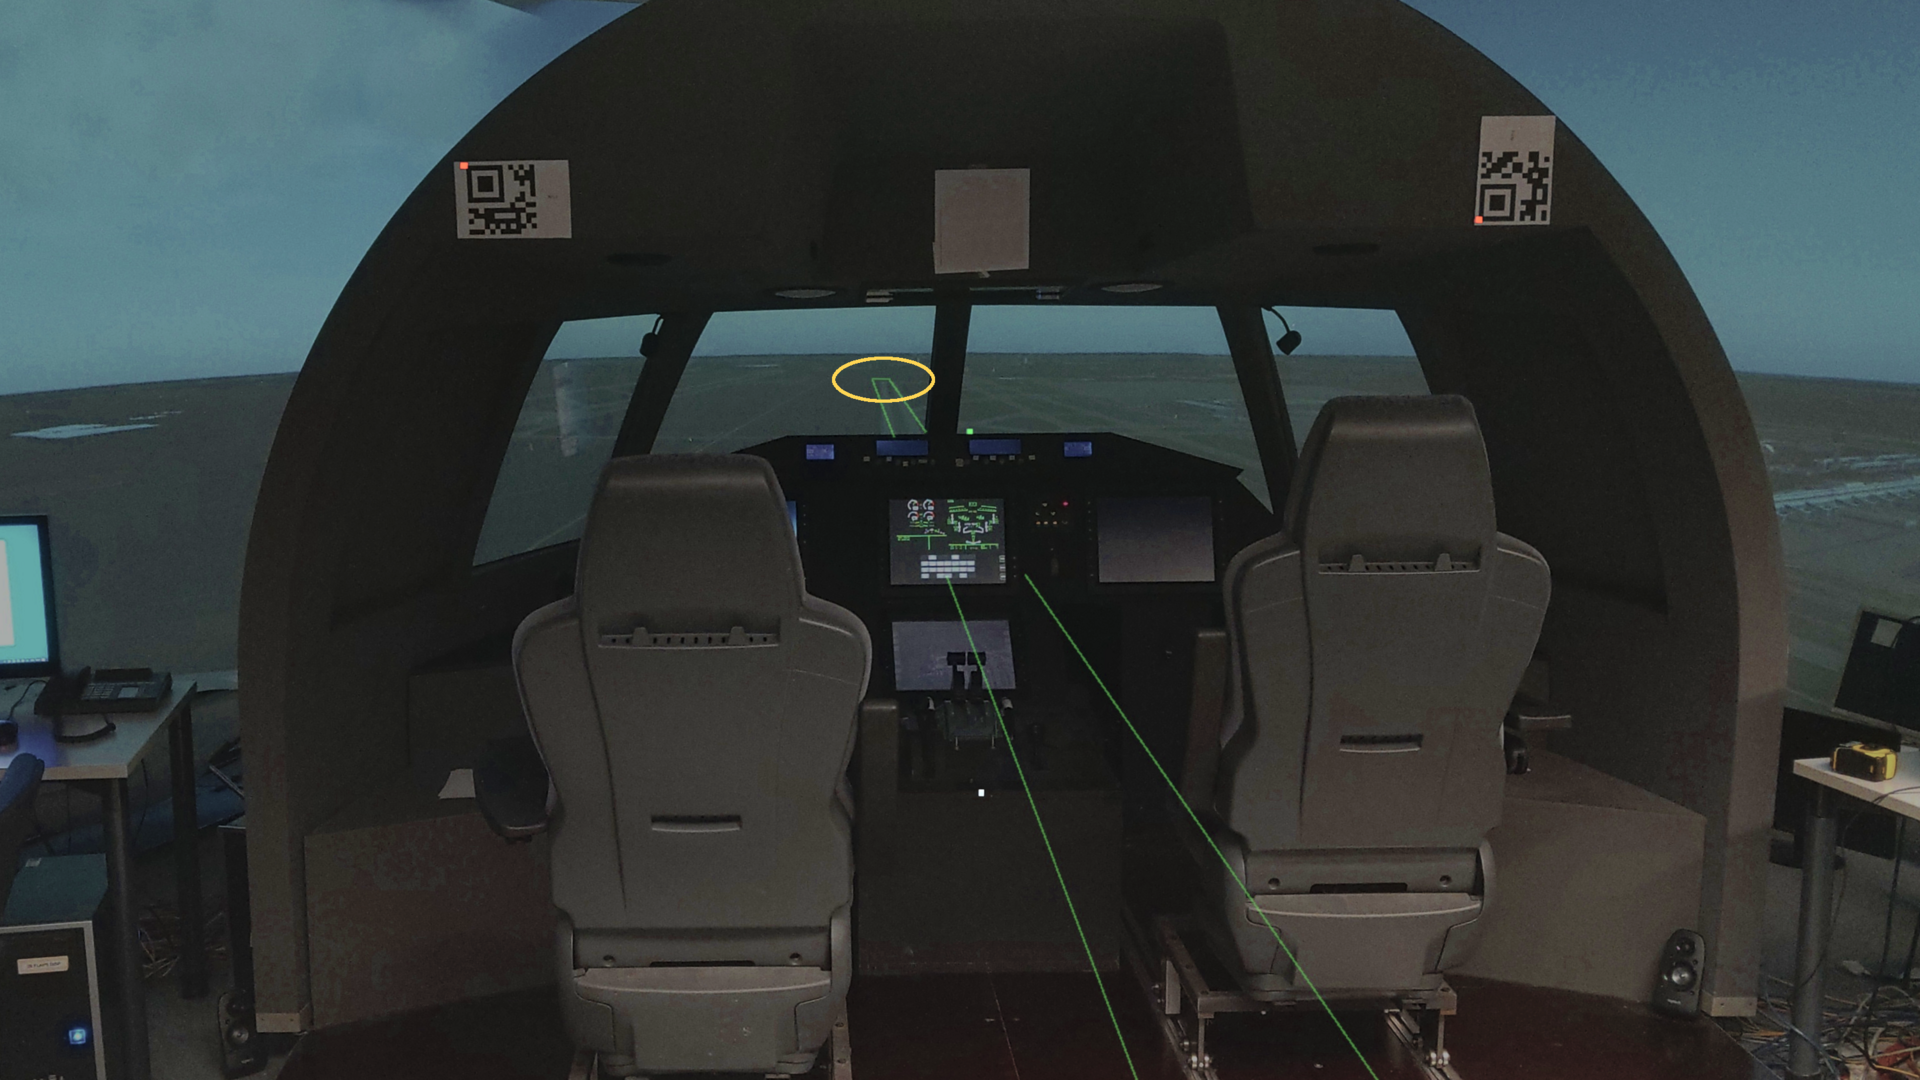
\includegraphics[width=0.8\textwidth]{munich-runway-no-interpolation-2.png}
  \caption{An image taken from the Hololens that shows a \gls{geofixedaug} highlighting the runway of an airport and the error induced by the combination of the limited number of vertices of the mesh and the projection applied by \gls{holoassist}. The vertices submitted through the \gls{API} (two are in the orange circle) are placed correctly, but they are connected with straight lines that do not follow the cylindrical projection screen.}\label{fig:munigh_runway_highligted_projection_not_interpolated.png}
\end{figure}

This problem can be solved by adding additional vertices to the mesh in intermediate positions between the original four vertices: in this way, each of the intermediate points will be projected to the cylinder and the error due to the fact that they are connected by straight lines will be less evident, as shown in \autoref{fig:munich_runway_interpolated.png}.

\begin{figure}
  \centering
  \subfloat[Coarse automatic interpolation]{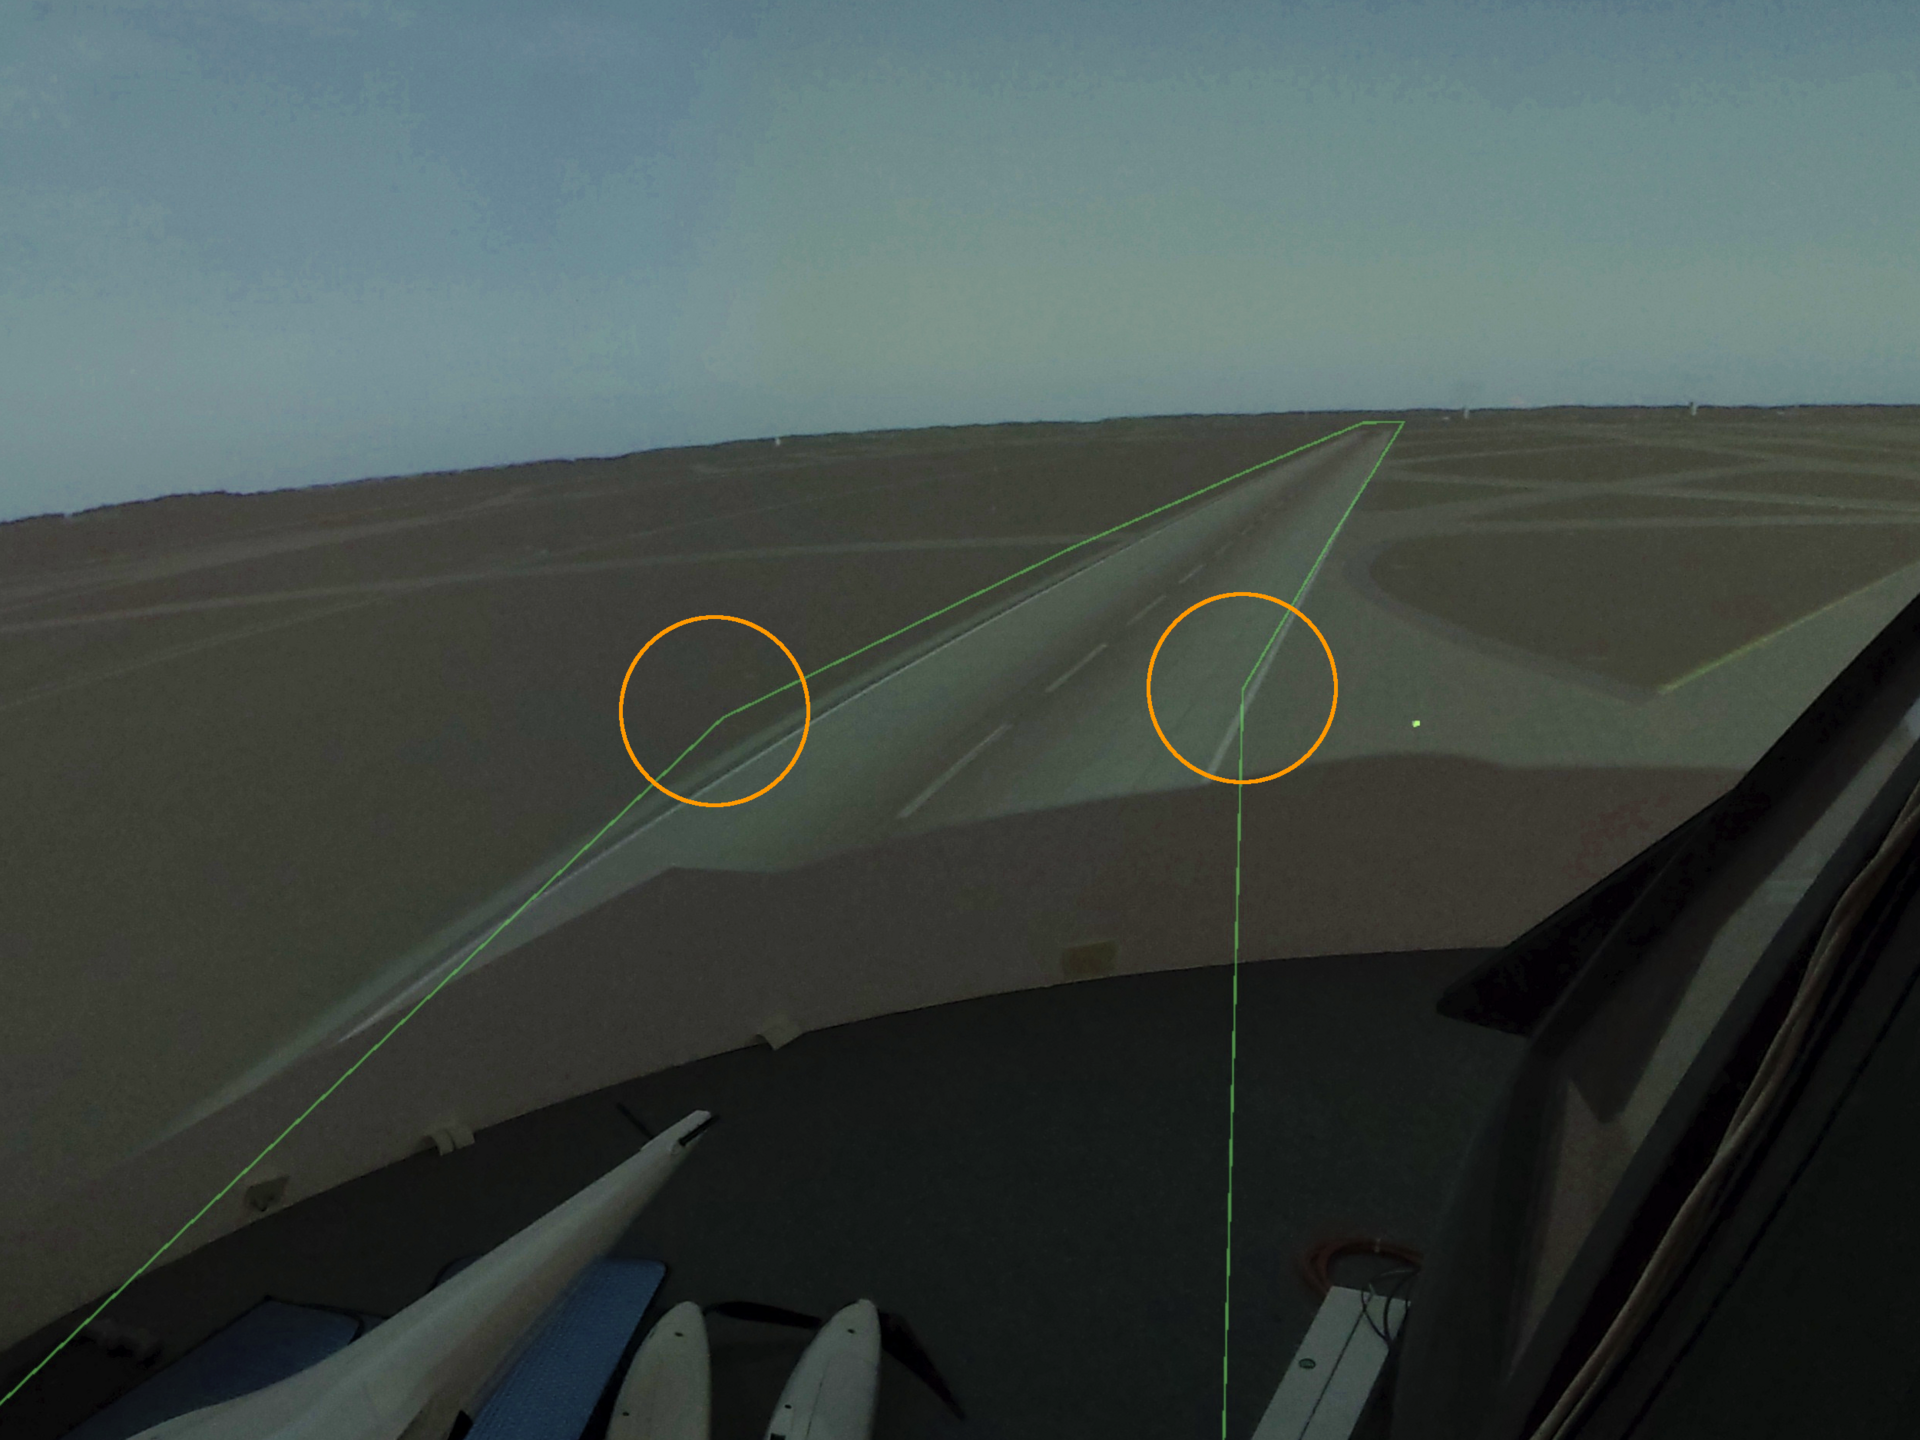
\includegraphics[height=0.35\textwidth]{progressive-interpolation-200m.png}}
  \hfill
  \subfloat[Fine automatic interpolation]{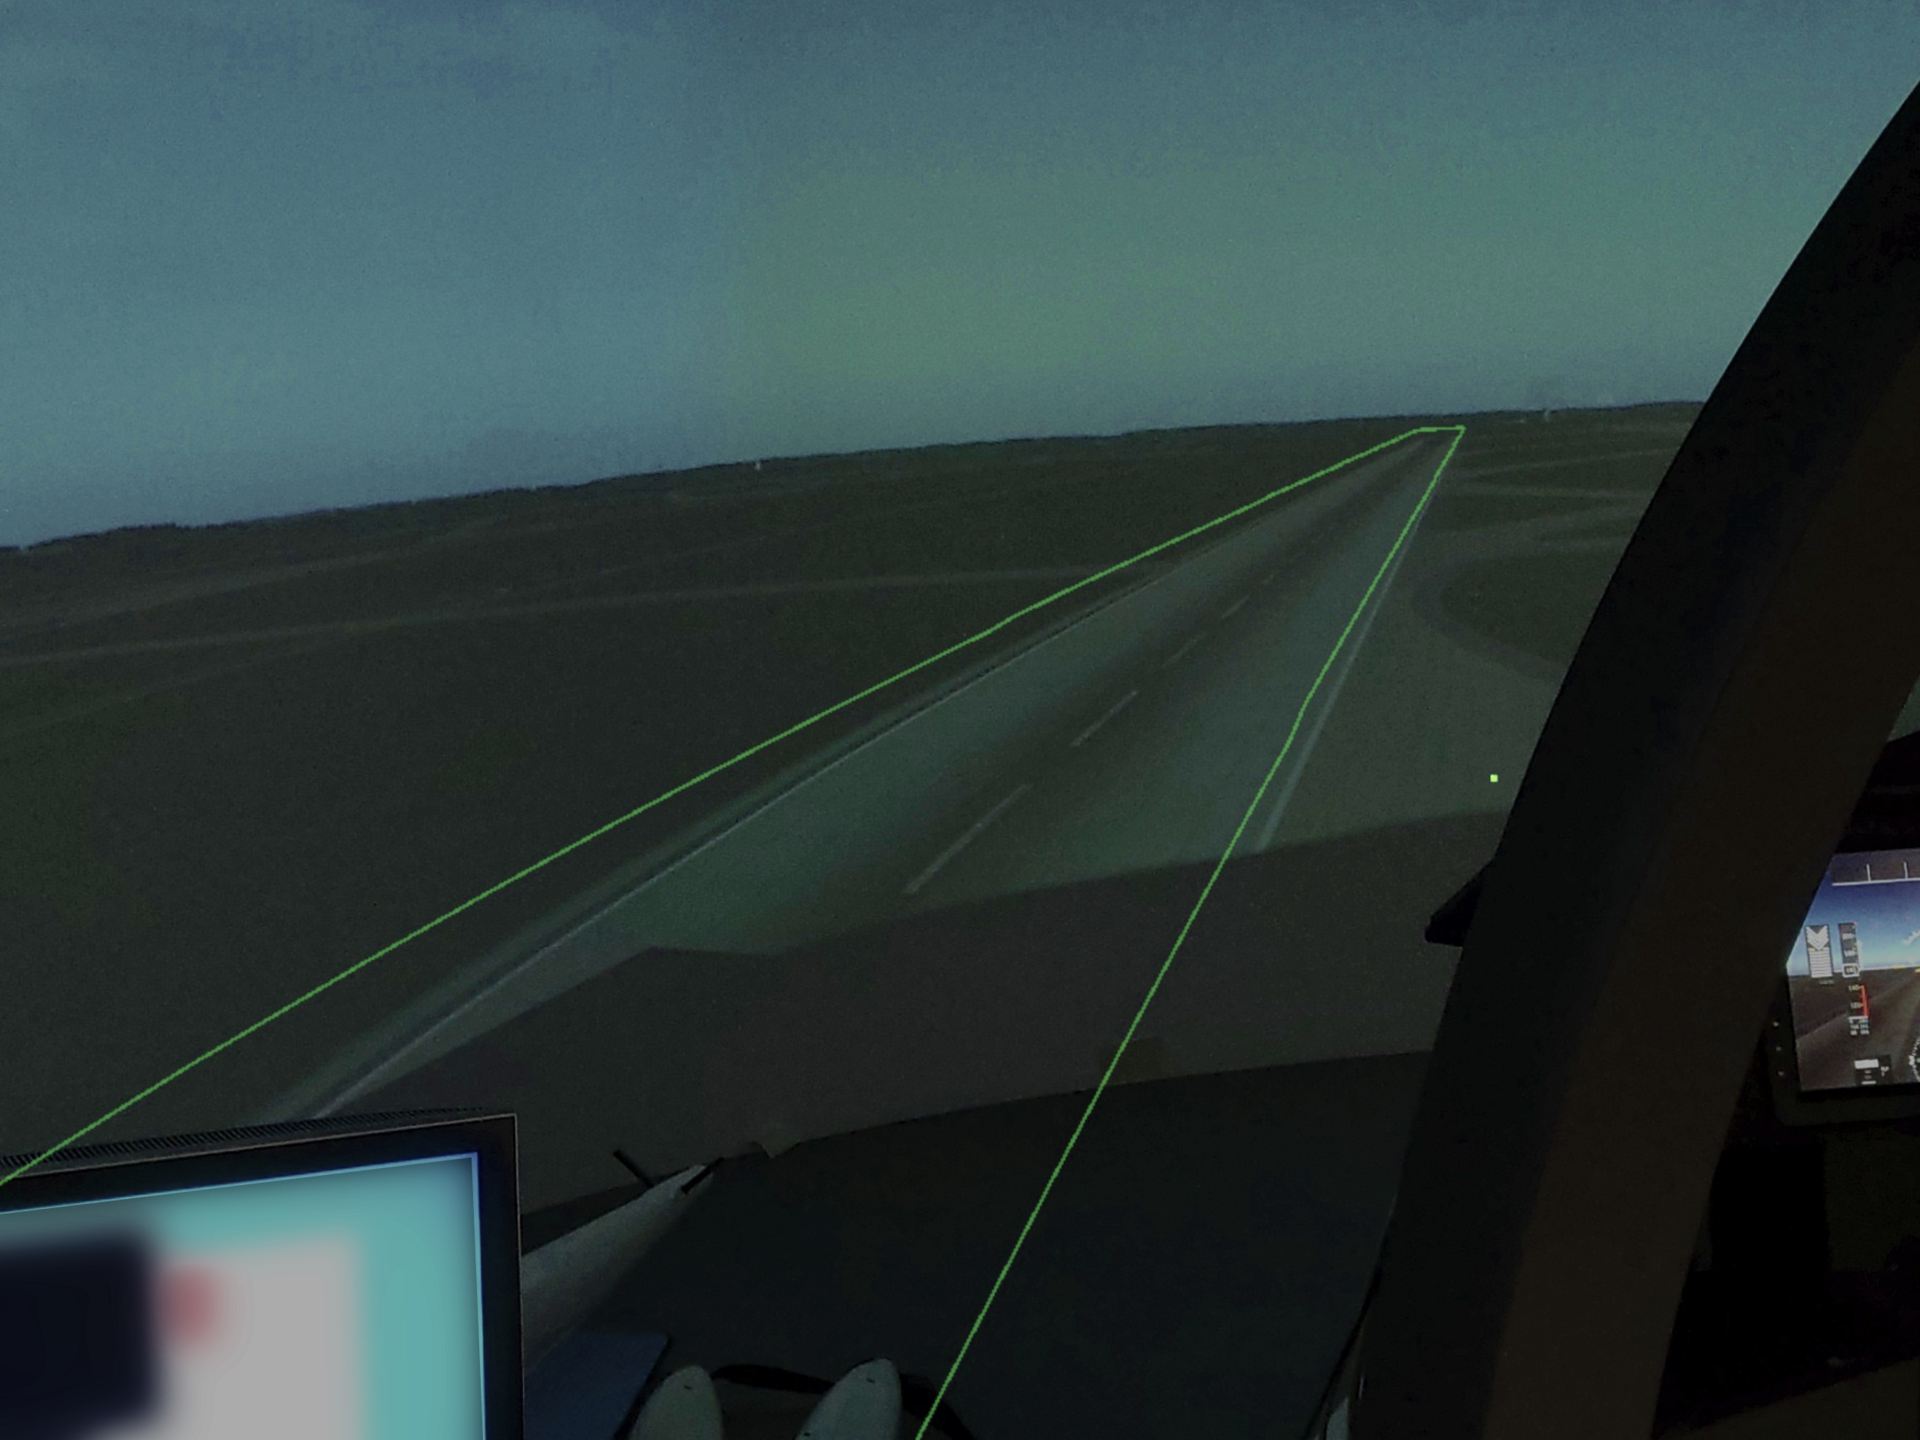
\includegraphics[height=0.35\textwidth]{progressive-interpolation-20m.png}}
  \caption{An image taken from the Hololens that shows how adding intermediate vertices allows the projection to behave as expected. As the coarse interpolation shows, the additional added vertices (shown in the orange circle) are correctly projected on the cylindrical screen, but there still are not enough vertices to provide a sufficiently smooth result.}
\label{fig:munich_runway_interpolated.png}
\end{figure}

However, forcing the user to deal with this problem (which effectively is an implementation detail of \gls{holoassist}) for every \gls{geofixedaug} that is created goes against the basic principle of making it easy for \gls{holoassist} users to create \gls{AR} experiences. Therefore, \gls{holoassist} performs this interpolation automatically by default when a \gls{gfelm} is created through its \gls{API}. Nevertheless, users working on more advanced use cases are still free to specify a maximum real-world distance between vertices after the interpolation and, if preferred, to opt-out of this automatic procedure entirely.

In order to implement this, the interpolation routine assumes a mesh with line topology, as the current version of \gls{holoassist} only supports that kind of topology (see \autoref{sec:projection_error}). This means that, for every \gls{gfelm}, the list of indices can be seen as a list of pairs of numbers, with each pair denoting a line segment that could potentially have to be interpolated. Therefore, after converting the vertices to the \gls{ECEF} \gls{CRS} as described in \autoref{eq:externallinemeshvertextoecef}, \gls{holoassist} goes through each of these line segments and, if needed, adds intermediate vertices via linear interpolation. More concretely, for each pair of indices that denotes a segment, let $\mathbf{v}_{\text{ECEF}}$ and $\mathbf{u}_{\text{ECEF}}$ be the coordinates of the vertices forming that segment in the \gls{ECEF} \gls{CRS}. Since \gls{ECEF} is an Euclidean space, the length of this segment can be computed with the Euclidean distance of these two points. If this value is above a certain threshold $t \in \mathbb{R}$ chosen by the user:

\begin{equation}
    \left \lVert \mathbf{v}_{\text{ECEF}} - \mathbf{u}_{\text{ECEF}} \right \rVert \geq t
\end{equation}

Then the segment is divided in $n$ equal sized pieces with:

\begin{equation}
    n = \left\lceil \frac{\left\lVert \mathbf{v}_{\text{ECEF}} - \mathbf{u}_{\text{ECEF}}\right\rVert}{t} \right\rceil
\end{equation}

Each of the new intermediate point $\mathbf{w}_i$ is computed by linear interpolation:

\begin{equation}
    \mathbf{w}_i = \mathbf{v}_{\text{ECEF}} + \left(\frac{1}{n} \cdot i\right) \left(\mathbf{u}_{\text{ECEF}} - \mathbf{v}_{\text{ECEF}}\right)
\end{equation}

These intermediate vertices are added to the mesh in a way that is transparent to the \gls{API} user and the indices are patched to correctly use also these intermediate vertices. This interpolation happens only once when the user changes the mesh.

\subsection{Measuring the simulator's parameters}\label{sec:obtaining_rfs_measures}

As described in \autoref{sec:projection_error}, a number of simulator-specific parameters are required to correctly compute the projection that \gls{holoassist} must apply. In commercial simulators these parameters are usually available as part of the documentation and are therefore straightforward to obtain. However, the simulator in which \gls{holoassist} has been tested (shown in all the previous pictures) is a research one, and has been built incrementally over several years from multiple different researchers involved in different projects: this results in a lack of official documentation and in the necessity of figuring out these parameters in an alternative way.

The most intuitive approach involves a tape measure, but the structure and scale of the simulator make this difficult. Determining exactly whether the projector screen is actually cylindrical, where the center of such cylinder is and how to measure its diameter/radius is not straightforward, as it requires measuring lengths across the whole room, with limited maneuver space and potentially intersecting various physical objects with irregular surfaces that cannot be moved (like the simulator cockpit itself). It was therefore decided to determine these parameters indirectly, by using the simulator's 3D scan acquired as described in \autoref{section:acquiring_digital_double}. After opening the 3D scan in Blender, its \enquote{cursor} tool was used to obtain the virtual 3D position of a number of points on the projector screen, as shown in \autoref{fig:acquiring_cylinder_points.png}.

\begin{figure}
  \centering
  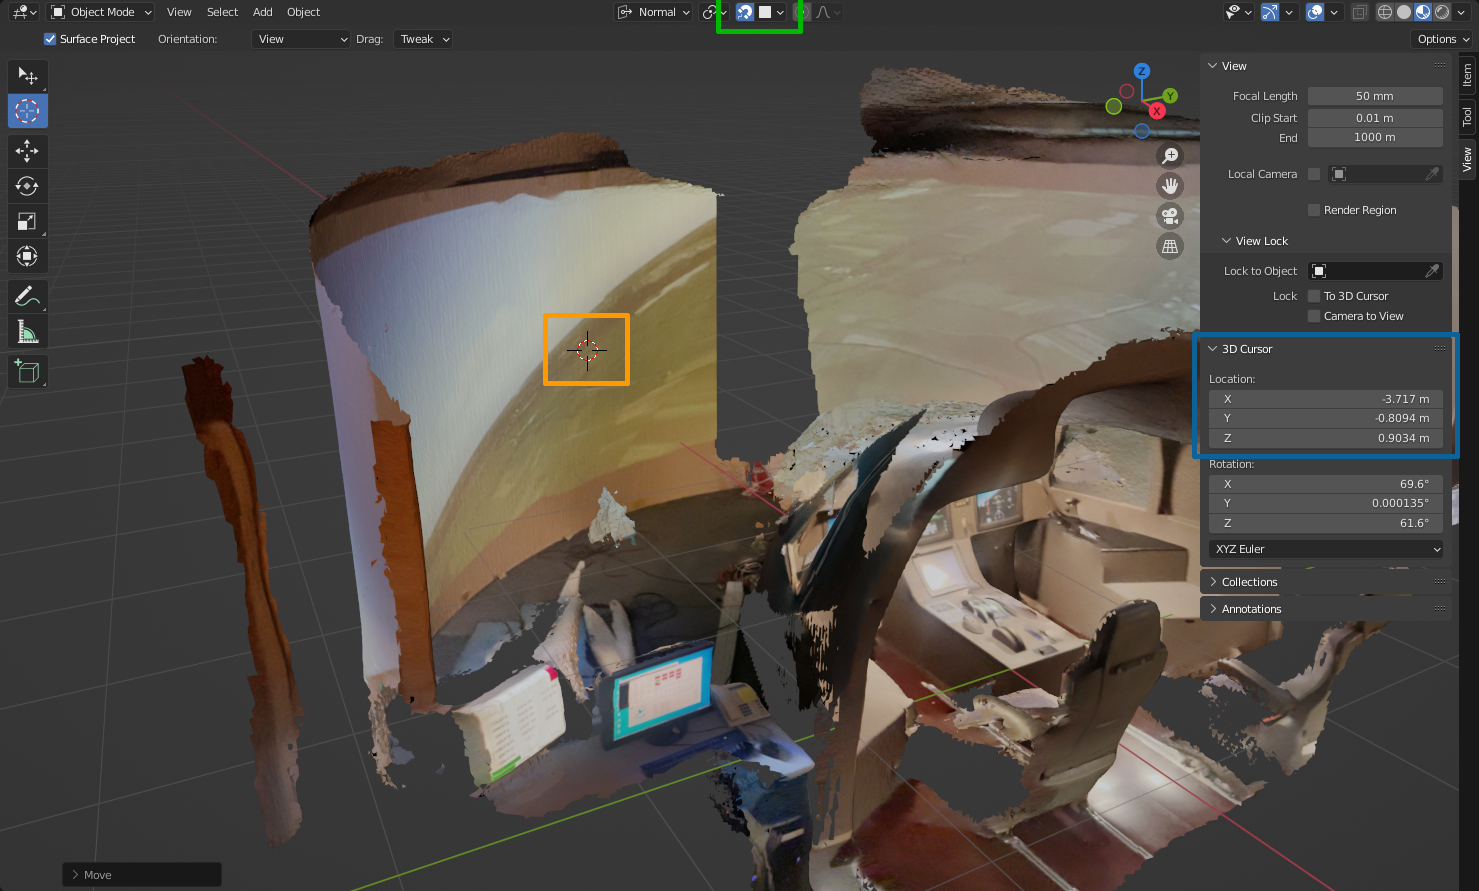
\includegraphics[width=0.6\textwidth]{acquiring_cylinder_points.png}
  \caption{After importing the 3D scan in Blender, the \enquote{cursor} tool (shown in the orange box) can be used to obtain the coordinates of various points on the 3D model. In this case, the \enquote{snap} feature of the cursor is enabled (green box): this allows the cursor to stick to the faces of the model. On the right (blue box), Blender allows to retrieve the current position of the cursor.}\label{fig:acquiring_cylinder_points.png}
\end{figure}

For each of these points, the Y coordinate has been discarded and the X and Z coordinates have been used to determine the best fitting circle, obtaining both the cylinder center and the cylinder radius. As the result in \autoref{fig:it_is_not_a_cylinder.png} clearly shows, the projector screen is definitely not cylindrical and would be better approximated with an elliptic cylinder. However, since this would require deriving a different projection with respect to the one shown in \autoref{sec:projection_error} and since the augmentations were visually mostly correct also by keeping the regular cylinder projection, this improvement was not implemented and the parameters of the best fitting circle were used. Nevertheless, if the user moves outside the simulator cockpit the error is significantly more visible, as shown in \autoref{fig:aug_it_is_not_a_cylinder.png}.

\begin{figure}
  \centering
  \begin{filecontents}{bfc_real_points.dat}
  -3.786 -0.5533
  -3.114 -1.833
  -3.533 -1.192
  -3.116 2.329
  -3.424 1.926
  -3.310 2.07
  -3.392 1.963
  -3.679 1.449
  -3.890 0.3203
  -3.525 -1.217
  -3.786 -0.553
  -3.114 -1.833
  -3.533 -1.192
  -3.116 2.329
  -3.424 1.926
  -3.310 2.070
  -3.392 1.963
  -3.679 1.449
  -3.890 0.320
  -3.525 -1.217
  -1.050 -2.874
  -2.193 -2.565
  -2.854 -2.118
  -1.777 3.324
  -2.018 3.154
  -2.537 2.840
\end{filecontents}

\begin{tikzpicture}
  \definecolor{myblue}{RGB}{13,98,153}
  \definecolor{myorange}{RGB}{255,153,0}

  \begin{axis}[
      width=0.48\textwidth,
      height=0.48\textwidth,
      xmin=-5, xmax=5,
      ymin=-5, ymax=5,
      xlabel={X},
      ylabel={Z}
    ]
    \addplot+[only marks, myblue] table [x index=0,y index=1] {bfc_real_points.dat};
    \addlegendentry{Measured points};
    \draw[myorange] (axis cs:0,0.2372135716) circle [radius=3.815579435];
    \addlegendimage{line width=0.2mm,color=myorange}
    \addlegendentry{Best fitting circle};
  \end{axis}
\end{tikzpicture}
  \caption{The plot obtained by trying to fit a circle to the points on the projection screen measured using the 3D scan. As it can be seen, the measured point are not really on a circumference and rather form an ellipse.}\label{fig:it_is_not_a_cylinder.png}
\end{figure}

\begin{figure}
  \centering
  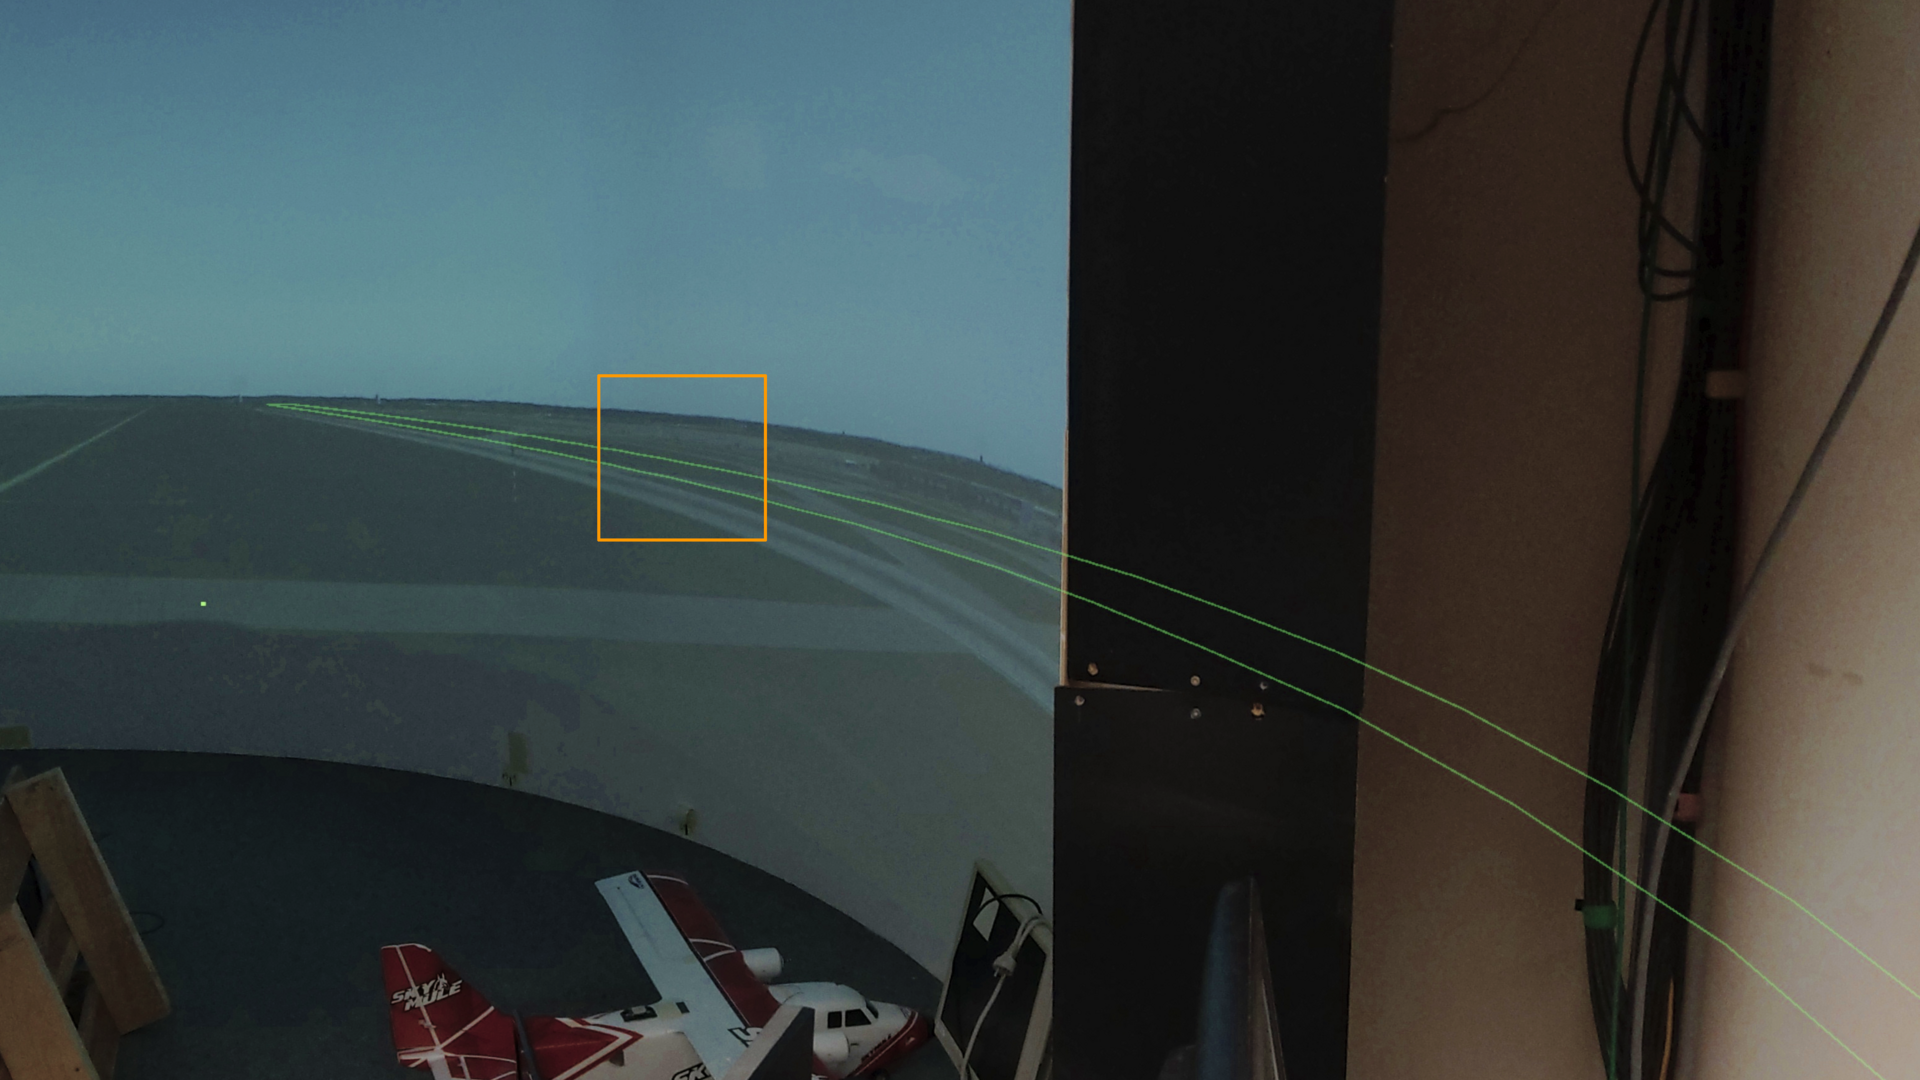
\includegraphics[width=0.7\textwidth]{its-not-a-cylinder.png}
  \caption{Image taken from the point of view of the Hololens that shows the error between the computed cylinder and the real surface of the projector screen. Since it is difficult to show in a static image, the point in which the projection cylinder \enquote{goes behind} the real projection screen is highlighted in orange: the augmentation on the right of this point is only visible because the spatial awareness feature of the Hololens is disabled. Inside the simulator cockpit this error is visually much less relevant.}\label{fig:aug_it_is_not_a_cylinder.png}
\end{figure}

The last parameters to determine are the \gls{PEP} and the airplane center of mass. The rigid offset between these two points has been obtained from the simulator engine configuration, as it is a parameter of the simulation. The \gls{PEP} was then placed in roughly the correct position with respect to the simulator digital double, and its position was further refined manually via the \gls{remoteunityeditor} described in \autoref{section:developerutilities} until the \gls{geofixedaug} would visually match with the geographical features shown on the projection screen by the simulator. While doing this, it is important to test the positioning of the \gls{PEP} by looking at the same augmentation from several different airplane positions and orientations, as it easily happens that the augmentation appears to be completely aligned with real world features from one aircraft position but then loose the alignment as soon as the position changes.

\subsection{Limitations due to floating-point precision}

The transformations to convert a \gls{ECEF} point to Unity coordinates and to project it on the cylindrical surface can be performed in \texttt{float} or \texttt{double} precision and need be executed every frame either on the CPU or on the GPU in a vertex shader. Due hardware limitations of the current version of the Hololens, the device's GPU only supports \texttt{float} operations. It was therefore decided to implement a GPU-based version of these transformations that uses \texttt{float} precision and a CPU-based version that uses \texttt{double} precision, and then compare the results. As can be seen in \autoref{fig:float_vs_double.png}, when using the higher-precision version the result is smoother, both spatially and temporally\footnote{Although this second aspect is more difficult to show in a static medium like a printed thesis.}. This is likely due to the fact that \text{ECEF} coordinates tend to be fairly big numbers (in absolute value) whereas the final Unity coordinates tend to be fairly small: in this situation, \texttt{float} arithmetic easily leads to a loss of precision that manifests with these artifacts. On the other side, the GPU implementation should be faster, as vertex shaders are designed exactly to perform this kind of computation for every vertex. However, since both the CPU-based and the GPU-based implementation are performant enough to achieve a stable framerate for the currently developed \glspl{geofixedaug}, the performance difference was not tested in details.

Future versions of the Hololens should include GPU support for \texttt{double} precision operations and should remove the necessity of choosing between visual quality and performance.

\begin{figure}
  \centering
  \subfloat[32-bit float precision]{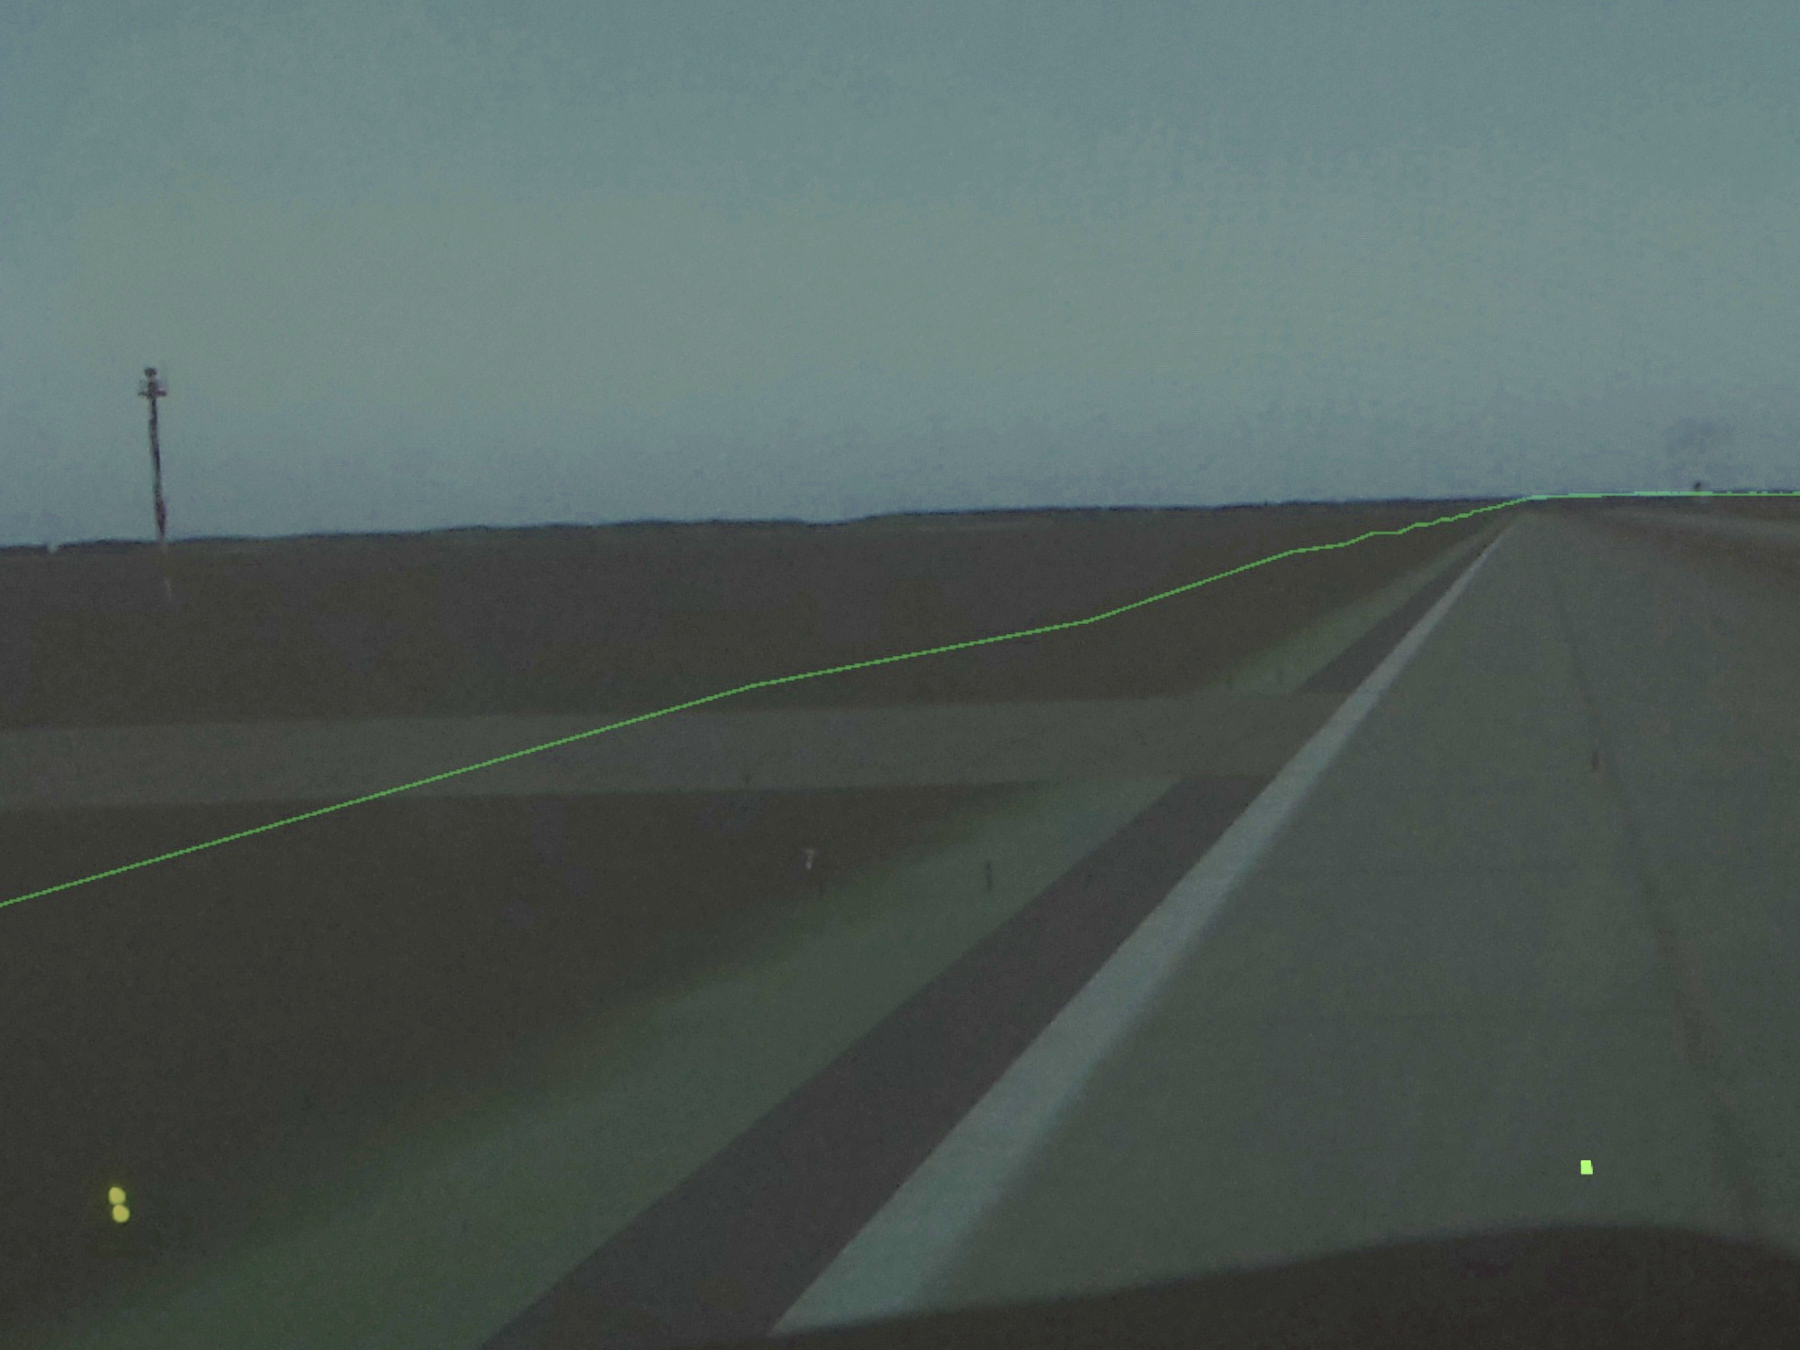
\includegraphics[height=0.35\textwidth]{runway-32bit.png}}
  \hfill
  \subfloat[64-bit double precision]{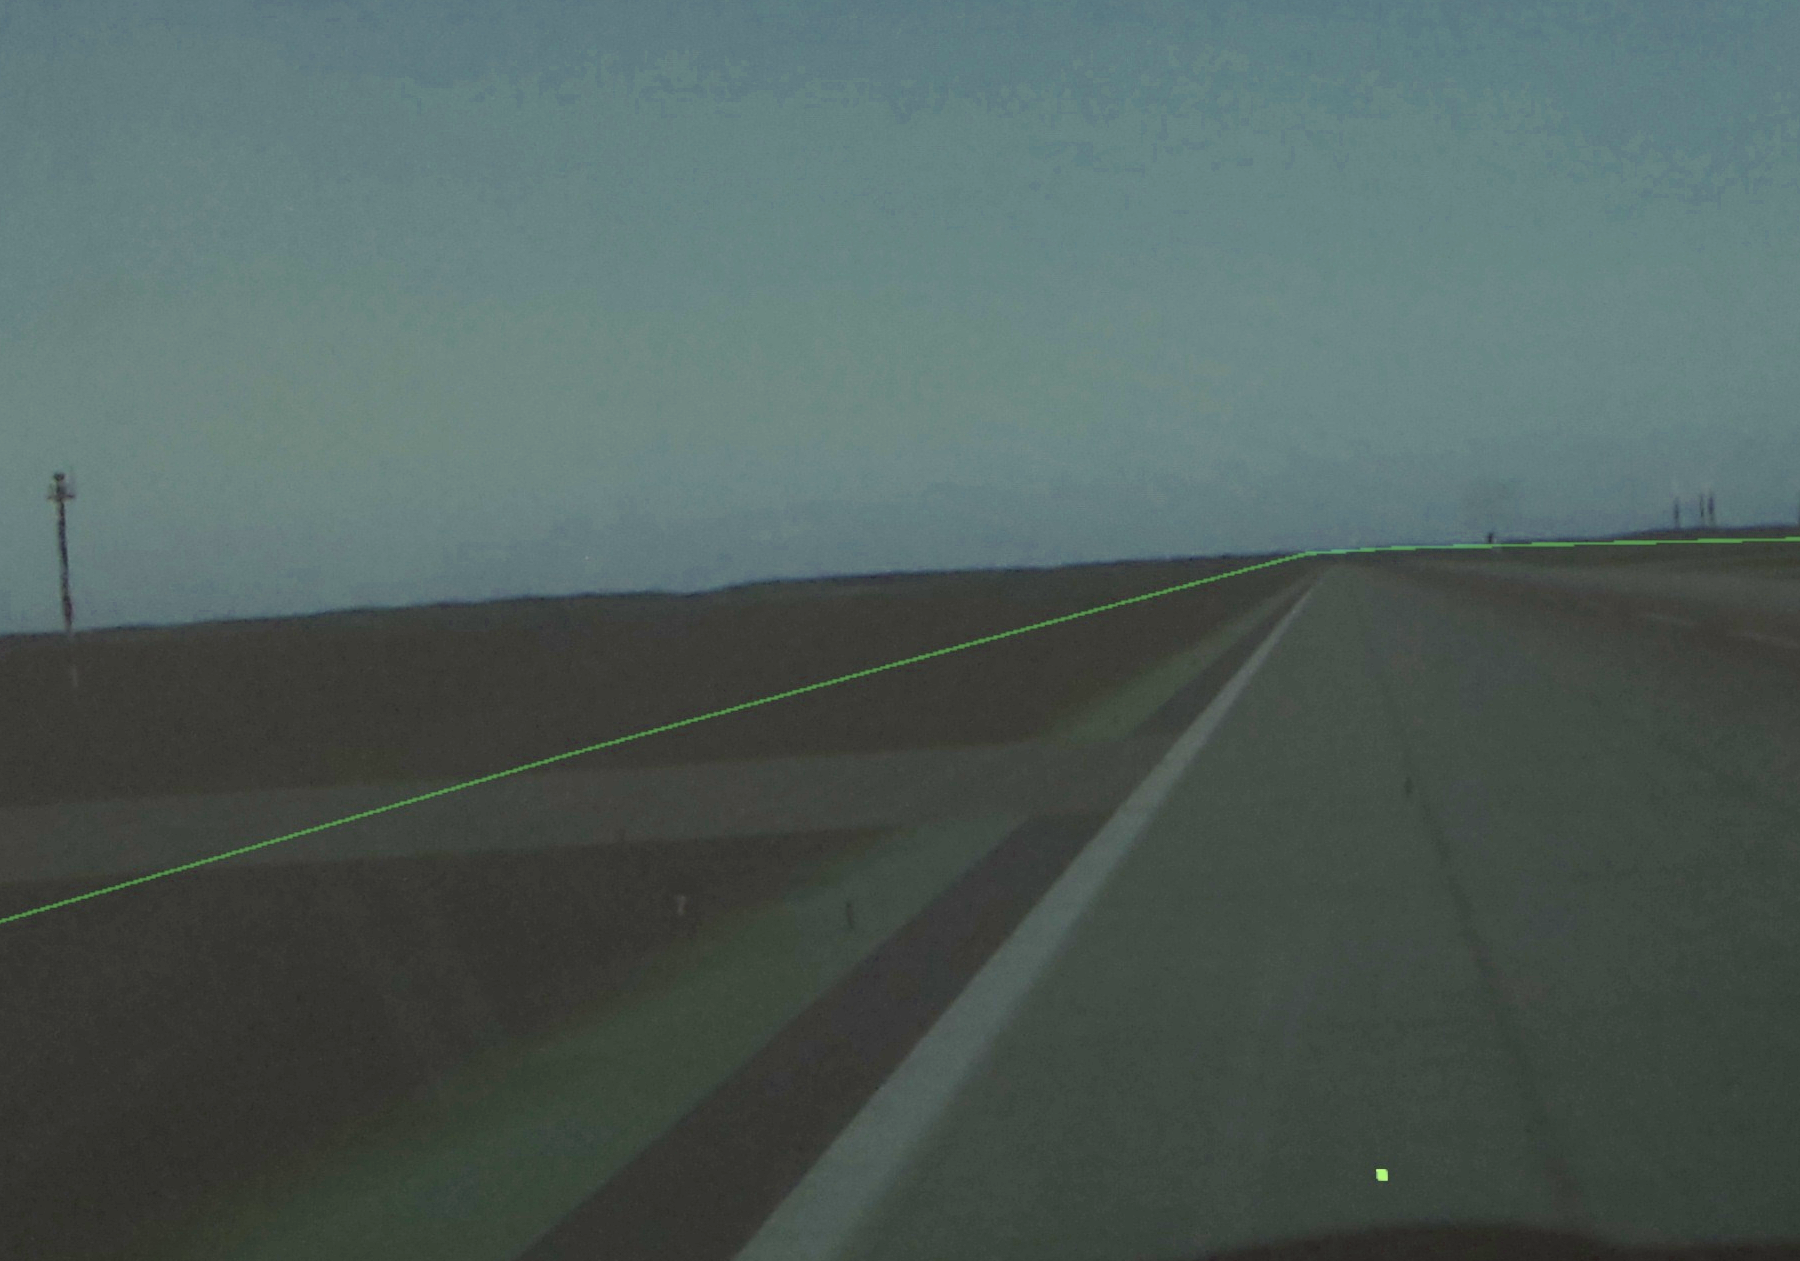
\includegraphics[height=0.35\textwidth]{runway-64bit.png}}
  \caption{Images acquired by the Hololens that show the same \gls{geofixedaug} rendered with the two different precisions. The 32-bit version presents some artifacts. The temporal inconsistency of these artifacts manifests as a small jitter of the \gls{geofixedaug} around the correct position.}\label{fig:float_vs_double.png}
\end{figure}

\section{Plane-fixed augmentations}\label{section:planefixedaugmentations}

The other kind of augmentations supported by \gls{holoassist} is called \enquote{\gls{planefixedaug}} and consist of augmentations that are shown in a fixed position with respect to the airplane's cockpit. Some envisioned use cases for this kind of augmentations are highlighting commands inside the cockpit or showing virtual displays to the pilot.

The setup described in \autoref{section:aligning_virtual_with_real_world} and \autoref{section:acquiring_digital_double} already offers a coordinate system aligned with the simulator digital double (and therefore with the real simulator cockpit) in which this kind of augmentations can be shown. Therefore, offering this functionality to the user only requires extending \gls{holoassist}'s \gls{API} to enable creating, editing and deleting normal 3D meshes (that is, instances of \texttt{UnityEngine.CoreModule.Mesh}), which are then added to the Unity scene at a position and orientation specified on mesh creation. The resulting \gls{API} is very close to the one for \glspl{geofixedaug} and allows to modify the vertex list and index list of every mesh created through the \gls{API}. The main difference is that instead of defining vertices as \texttt{GeoFixedVertex}, they only consist of a 3D position and a color. In this case, neither interpolation nor projection is required.

An example of a \gls{planefixedaug} which highlights the gear lever is shown in \autoref{fig:plane_fixed_aug_example.png}.

\begin{figure}
  \centering
  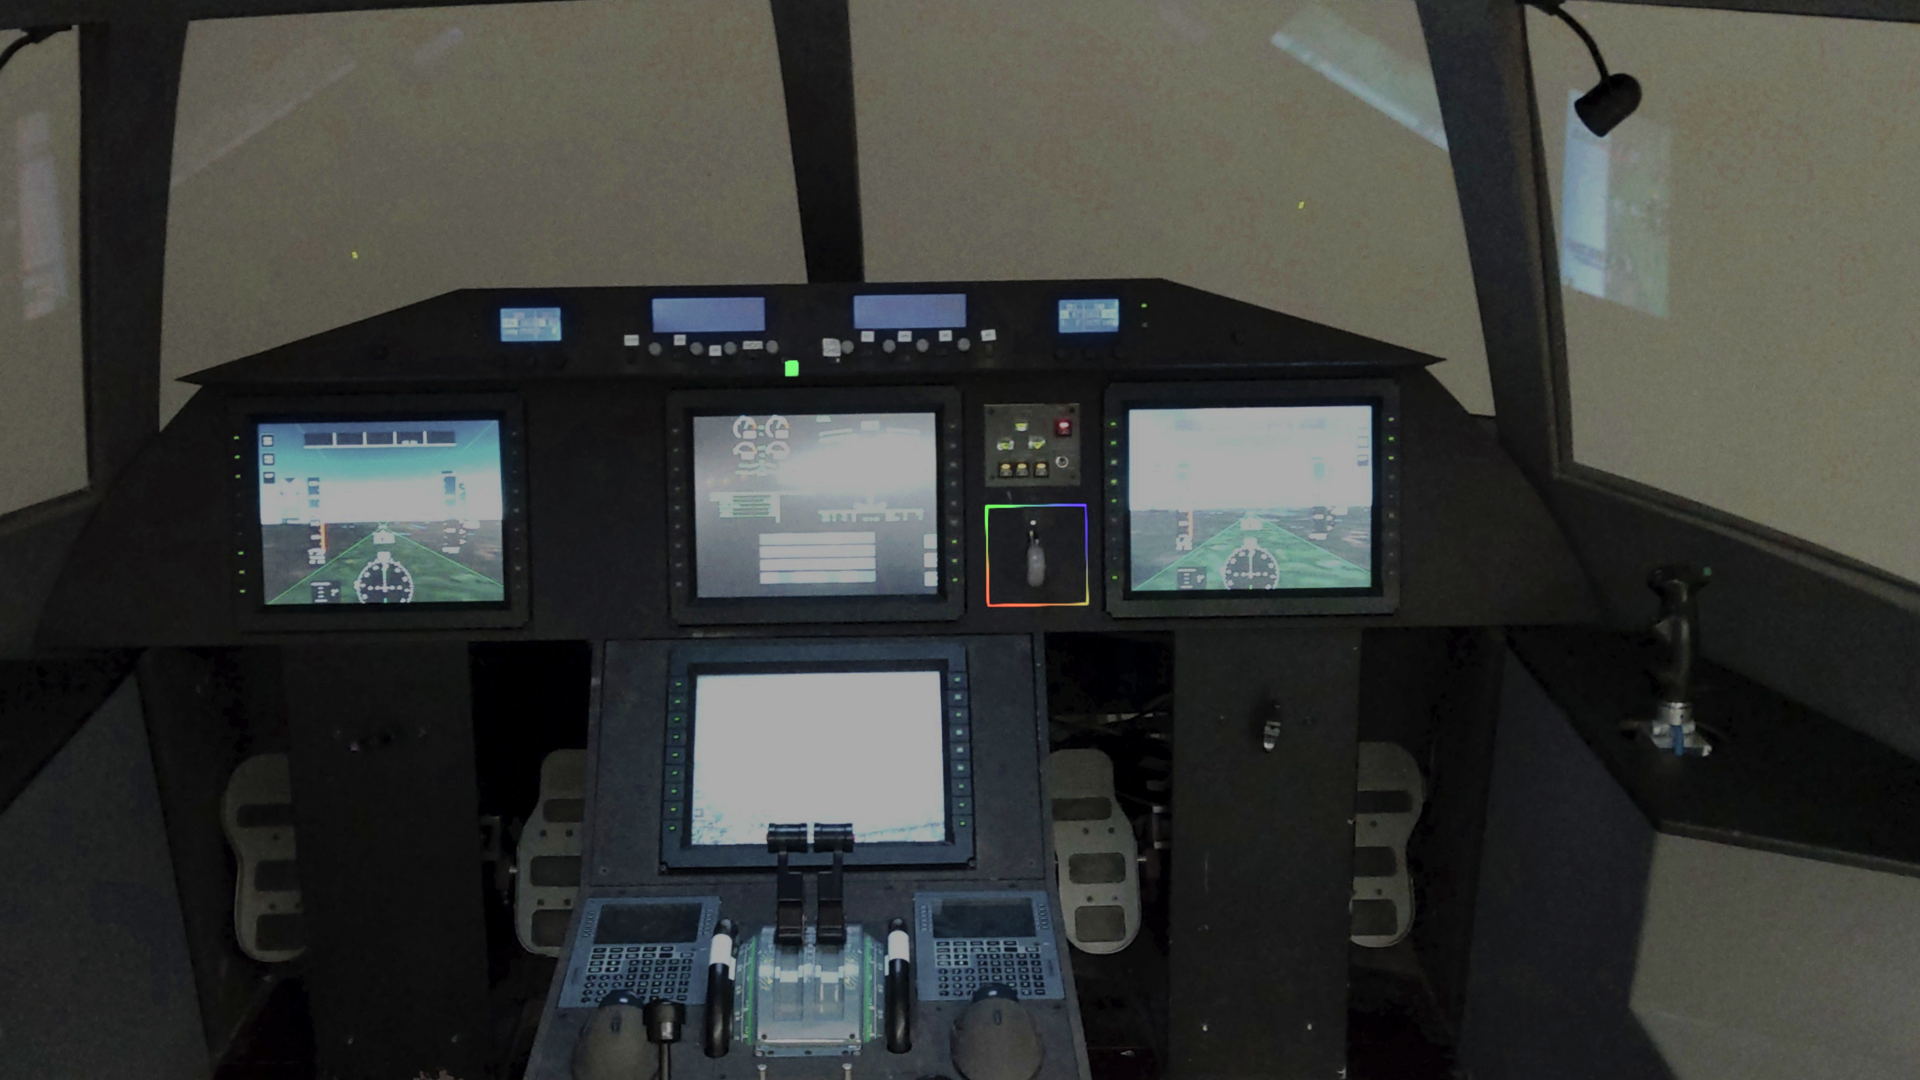
\includegraphics[width=0.75\textwidth]{plane-fixed-augmentations.png}
  \caption{Image acquired from the Hololens that shows an example \gls{planefixedaug} that consists of a colored rectangular outline surrounding the gear lever near the center of the picture.}\label{fig:plane_fixed_aug_example.png}
\end{figure}

The main problem posed by this kind of augmentation regards the precision required: although the alignment between the real and the virtual world is fairly precise, it still has an error of around $1$cm. Therefore, the precision is not sufficient to highlight particularly small elements, like a single knob in the cockpit. This partially limits the currently available use cases for which \glspl{planefixedaug} can be used.

Due to the 3D scan acquired as described in \autoref{section:acquiring_digital_double}, designing a \gls{planefixedaug} is fairly easy: it is sufficient to open the 3D scan in a digital modeling tool like Blender and use the software to design the desired augmentation as a normal 3D mesh, using the imported scan as a reference for dimensions and positions. The designed mesh can then be exported (e.g.\ as a Wavefront OBJ file\cite{japan_industrial_standards_microqr_nodate}) and drawn via the \gls{holoassist} \gls{API}. This is further simplified by the fact that the 3D scan not only contains the 3D geometry of the simulator, but also a projected texture which shows the real-world color of each point of the scan as shown in \autoref{fig:simulator_3d_scan.png}: this allows to distinguish small scale details that do now appear in the raw geometry. An example of an augmentation drawn in Blender is available in \autoref{fig:plane_fixed_aug_authoring_example.png}.

\begin{figure}
  \centering
  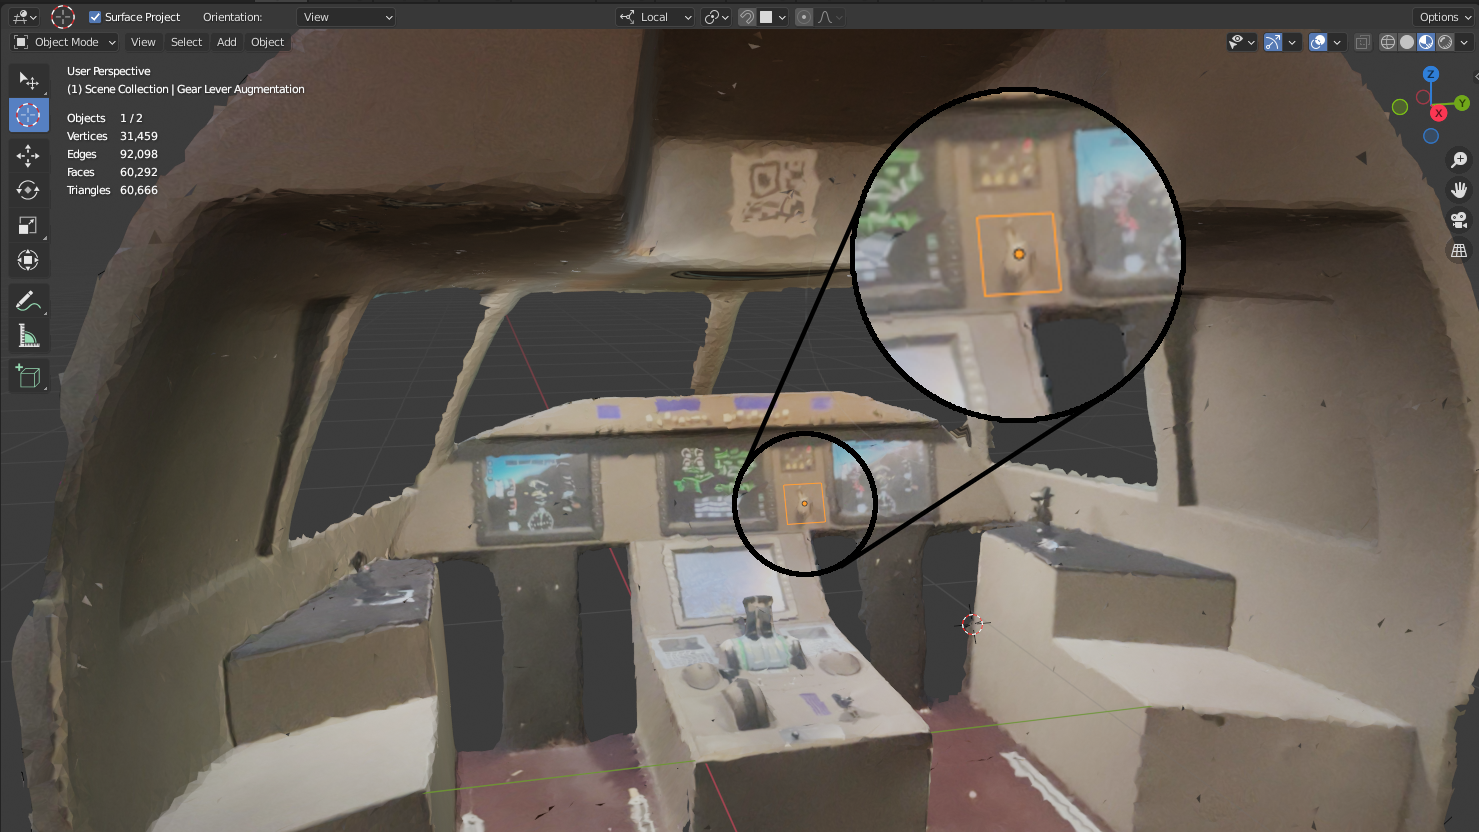
\includegraphics[width=0.75\textwidth]{plane-fixed-aug-blender.png}
  \caption{The gear lever \gls{planefixedaug} as it appears in Blender. As it can be seen, the textured 3D scan is used as a base to draw the mesh. The result will then be exported and loaded through a \gls{holoassistapp}.}\label{fig:plane_fixed_aug_authoring_example.png}
\end{figure}

Creating this kind of augmentations without such a precise 3D scan would be much more cumbersome and time consuming: this is one of the reasons for which some of the 3D scan attempts described in \autoref{section:acquiring_digital_double} (like using the Hololens spatial awareness mesh) were discarded.

As a last remark, it should be noted that currently also \glspl{planefixedaug} are limited to only accept meshes with line topology. In this case, the limitation is not due to rendering issues, as in this case the normal pipeline would have worked without problems, but due to time-related constraints: supporting meshes with triangle topology would also have required an \gls{API} capable of supporting materials (to handle triangle colors, transparency and more). Designing such \gls{API} is time-consuming and, since \gls{planefixedaug} are a comparatively less important use case for \gls{holoassist}, it was decided to deprioritize this feature.

\section{Integrating a new simulator}\label{sec:integrating_new_sim}

\gls{holoassist} is designed in a way that allows integrating a new fixed-platform simulator with minimum additional effort. In order to do this, the first step is to acquire a 3D scan of the new simulator using a recent iPad\cite{apple_inc_ipad_nodate} (or, alternatively, the photogrammetry pipeline). If acquiring the whole simulator in a single step is too difficult, different partially-overlapping scans can be aligned with Meshlab's ICP tool\cite{zhang_fast_2021}. Blender can then be used to prepare a simplified occlusion mesh that can be exported to a Wavefront OBJ file.

The next step requires creating and printing at least two QR codes. They need to adhere to the \enquote{Micro QR Code}\cite{japan_industrial_standards_microqr_nodate} standard and have a printed size of at least $10\text{cm} \times 10\text{cm}$, the bigger the better. Each QR code must contain a string that matches the pattern \texttt{<simulator\_name>\--<number>}, where \texttt{<simulator\_name>} is a string identifying the simulator (and therefore equal among all the QR codes) and \texttt{<number>} is a progressive number. These QR codes need to be placed on the simulator according to a few criteria:

\begin{enumerate}
    \item The further they are away from each other the better.
    \item The relative offset between two QR codes should involve more than a single axis. If the offset can be described with a translation along a single one of the three main axes the resulting alignment will be sub-optimal.
    \item At least one QR code should not lie on the same plane, in order to improve the orientation estimation.
    \item The relative offset between the QR codes should be easy to measure.
\end{enumerate}

At this point, a new folder should be created inside the \gls{holoassist} code repository at the path \texttt{//Assets/Resources/Planes/<simulator\_name>}, where \texttt{<simulator\_name>} is the same string printed on the QR codes. Inside this folder, two files should be added: one is a \texttt{plane-mesh.obj} file that contains the occlusion mesh that was obtained from the 3D scan and one is a \texttt{plane-measures.json} file that contains all the simulator-specific parameters.

The first part of the \texttt{plane-measures.json} that should be filled regards the space pins. The numerical values for the first space pin can be chosen arbitrarily, but the other two need to match the real world offset between the QR codes that was previously measured. For example, imagine the real-world setup shown in \autoref{fig:rfs_qr_codes.png}, where the two QR codes are on the same plane, but one is rotated $90^{\circ}$ to the left (to ensure that the offset between them is on at least two axes). The relative distances between the QR codes are as shown in the figure. The space pin part of the JSON file for such a setup is shown in \autoref{lst:space_pins_virtual_positions_example_json}.

\begin{figure}
  \centering
  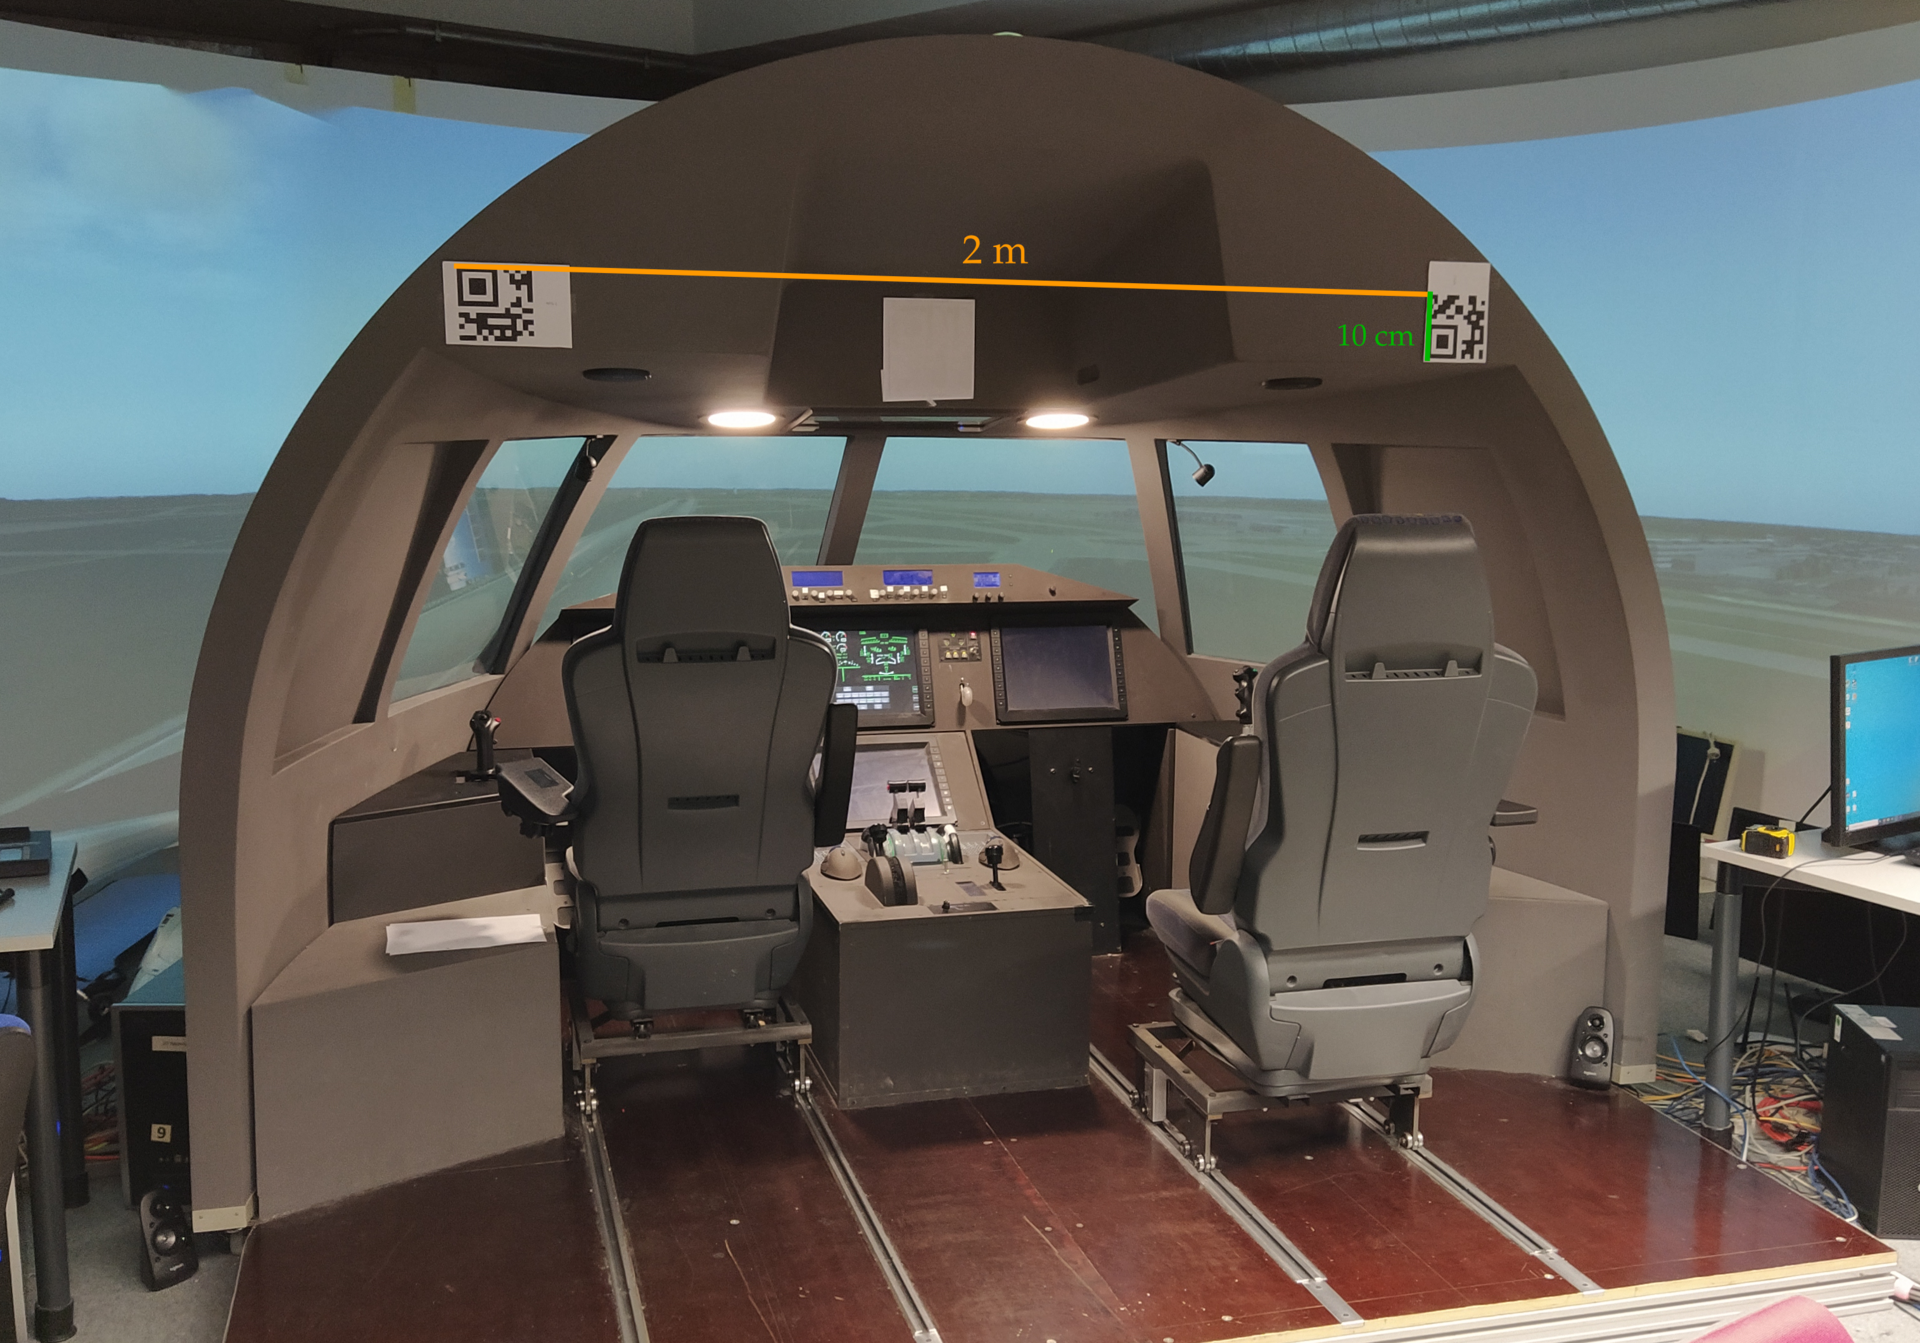
\includegraphics[width=0.8\textwidth]{real-world-qr-codes.png}
  \caption{An example real-world setup for placing the required QR codes.}\label{fig:rfs_qr_codes.png}
\end{figure}

\begin{figure}
  \centering
  \begin{tabular}{c}
  \begin{lstlisting}[language=json]
    {
        "spacePins": {
            "<simulator_name>-1": [ 0.0, 0.0, 0.0 ],
            "<simulator_name>-2": [ 2.0, 0.10, 0.0 ],
        },
        // other simulator-related information
    }
  \end{lstlisting}
  \end{tabular}
  \caption{An extract of the JSON file that describes the virtual positions of the space pins for the setup shown in \autoref{fig:rfs_qr_codes.png}.}\label{lst:space_pins_virtual_positions_example_json}
\end{figure}

Please note that for this QR code disposition and for this coordinate choice, the Z and Y axes of the resulting Unity coordinate system will be respectively aligned with the real simulator's cockpit longitudinal axis and vertical axis as required by \gls{holoassist} (see \autoref{sec:renderling_elm}). Running \gls{holoassist} at this point and scanning the QR codes should result in a small colored cube appearing in the top left corner of each QR code.

The next step entails correctly placing the simulator digital double in the virtual space. This can be done by specifying a random value for the \texttt{planeMesh} key of the JSON file. Then, after starting \gls{holoassist}, the mesh can be visually aligned by using the \gls{remoteunityeditor} (see \autoref{section:developerutilities}), which allows the live editing of position and rotation of Unity objects. The final position of the mesh can then be read and be written as the final value of the \texttt{planeMesh} key. At this point, \gls{holoassist} should be able to scan the QR codes and correctly place the digital double.

If the projector screen shape is not cylindrical, then an additional projection method should be implemented. If it instead is cylindrical, then the position of the cylinder center, cylinder radius and \gls{PEP} should be obtained, either from the simulator's documentation or as described in \autoref{sec:obtaining_rfs_measures}. Their position in Unity's frozen coordinate system should then be stored in the JSON file. Once again, refining these points (especially the cylinder radius) via the \gls{remoteunityeditor} is possible.

The last step entails ensuring that the simulator broadcasts the airplane position and orientation correctly to \gls{holoassist}. However, this is a simulator-specific step, and therefore cannot be detailed here. The required data format is available in \autoref{table:sim_status_update_udp_packet}. At this point, \gls{holoassist} should be ready to show augmentations in the new simulator.

This procedure has been used to succesfully integrate \gls{holoassist} in a second fixed-platform simulator available at the research institute in which this project was developed. The integration required only a couple of days of work, with the main difficulties being networking issues and finding the correct positioning of the \gls{PEP}.

\section{Developer utilities}\label{section:developerutilities}

While working on \gls{holoassist}, it was deemed useful to develop two additional utilities that would help simplifying the development process: the \gls{remoteunityeditor} and the simulator position updater.

The \gls{remoteunityeditor} is composed by two parts: a Unity \texttt{Component} that listens for some particular \gls{UDP} messages and a Rust application designed to be run on a computer and to interact with this component via the local network. The main use case for this utility is that, in some cases, it is very helpful to be able to wear the Hololens, start \gls{holoassist}, load some holograms and then modify the position and rotation of such holograms without having to recompile and redeploy the Unity application to the device. The \gls{remoteunityeditor} allows to select a Unity \texttt{GameObject} by name and then use the computer's keyboard to translate it or rotate it while \gls{holoassist} is running. Using a Bluetooth keyboard instead of a wired one lets the user easily tweak the position of holograms while moving around in the \gls{AR} experience and looking at them through the Hololens. This is useful, for example, for refining the position of \glspl{planefixedaug} or for tweaking the position of the \gls{PEP} as described in \autoref{sec:obtaining_rfs_measures}. It is also possible to dump the current position and orientation of a \texttt{GameObject} to a \gls{UDP} packet which can be received and inspected via Wireshark, allowing to retrieve the refined pose of any object of the scene. This \gls{UDP} packet is a UTF-8 encoded string which is automatically decoded by Wireshark and contains a self-descriptive JSON object.

Related to this is the possibility of using Wireshark to read debug \gls{UDP} packets sent from the Hololens to the computer. This is useful because, when compiled in release mode and deployed to the device, \gls{holoassist} is very difficult to debug. This is due to the fact that logs lack debug symbols, often are very minimal and do not report invocations \texttt{Debug.Log} (the standard logging utility in Unity). As a work around, \gls{holoassist} can send log messages via \gls{UDP}, which offers a limited way of debugging problems that only appear when the application is compiled in release mode or if the debug build is too slow to be usable. A late discovery was the possibility of enabling Unity Development Builds, which still apply all the release optimization but offer additional introspection capabilities, like showing the logs printed through \texttt{Debug.Log} and being able to profile the application through Unity's profiler.

The other utility that was developed is the \enquote{simulator position updater}, which allows to send simulator status updates to \gls{holoassist} without a real flight simulator broadcasting updates. This utility was created to enable the development of \gls{holoassist} also when working from home or when the simulator was being used by someone else. The application allows to quickly set the simulator position to a few hardcoded presets and to tweak the plane geographical position and orientation by using a keyboard. This is achieved by using the same \gls{UDP} interface through which real simulator status updates are received, using the packet structure described in \autoref{table:sim_status_update_udp_packet}. 